\documentclass[letterpaper]{article} % DO NOT CHANGE THIS
\usepackage[submission]{aaai2027}  % DO NOT CHANGE THIS
% The serif, sans-serif, and monospaced fonts are loaded automatically by
% aaai2027.sty (newtxtext, helvet, courier). DO NOT add \usepackage{times},
% \usepackage{helvet}, \usepackage{courier}, or any other font package.
\usepackage[hyphens]{url}  % DO NOT CHANGE THIS
\usepackage{graphicx} % DO NOT CHANGE THIS
\urlstyle{rm} % DO NOT CHANGE THIS
\def\UrlFont{\rm}  % DO NOT CHANGE THIS
\usepackage{natbib}  % DO NOT CHANGE THIS AND DO NOT ADD ANY OPTIONS TO IT
\usepackage{caption} % DO NOT CHANGE THIS AND DO NOT ADD ANY OPTIONS TO IT
\frenchspacing  % DO NOT CHANGE THIS
%
% These are recommended to typeset algorithms but not required. See the subsubsection on algorithms. Remove them if you don't have algorithms in your paper.
\usepackage{algorithm}
\usepackage{algorithmicx}
\usepackage{algpseudocode}
\algrenewcommand{\algorithmicrequire}{\textbf{Input:}}
\algrenewcommand{\algorithmicensure}{\textbf{Output:}}

%
% These are recommended to typeset listings but not required. See the subsubsection on listing. Remove this block if you don't have listings in your paper.
\usepackage{newfloat}
\usepackage{listings}
\DeclareCaptionStyle{ruled}{labelfont=normalfont,labelsep=colon,strut=off} % DO NOT CHANGE THIS
\lstset{%
	basicstyle={\footnotesize\ttfamily},% footnotesize acceptable for monospace
	numbers=left,numberstyle=\footnotesize,xleftmargin=2em,% show line numbers, remove this entire line if you don't want the numbers.
	aboveskip=0pt,belowskip=0pt,%
	showstringspaces=false,tabsize=2,breaklines=true}
\floatstyle{ruled}
\newfloat{listing}{tb}{lst}{}
\floatname{listing}{Listing}

%
% Recommended for better-looking tables
\usepackage{booktabs}

% Math, multi-row tables, subfigures, and cross-references used in the paper.
\usepackage{amsmath}
\usepackage{amssymb}
\usepackage{multirow}
\usepackage{subcaption}
\usepackage{cleveref}

% Theorem-like environments used in the paper.
\newtheorem{theorem}{Theorem}
\newtheorem{lemma}{Lemma}
\newtheorem{assumption}{Assumption}
\newtheorem{remark}{Remark}
\newtheorem{hypothesis}{Hypothesis}

% Capitalized names for \cref output.
\crefname{algorithm}{Algorithm}{Algorithms}
\crefname{equation}{Equation}{Equations}
\crefname{figure}{Figure}{Figures}
\crefname{table}{Table}{Tables}
\crefname{theorem}{Theorem}{Theorems}
\crefname{assumption}{Assumption}{Assumptions}
\crefname{lemma}{Lemma}{Lemmas}
\crefname{remark}{Remark}{Remarks}
\crefname{hypothesis}{Hypothesis}{Hypotheses}

%
% Keep the \pdfinfo as shown here. There's no need
% for you to add the /Title and /Author tags.
\pdfinfo{
/TemplateVersion (2027.1)
}

% DISALLOWED PACKAGES
% \usepackage{authblk} -- This package is specifically forbidden
% \usepackage{balance} -- This package is specifically forbidden
% \usepackage{CJK} -- This package is specifically forbidden
% \usepackage{float} -- This package is specifically forbidden
% \usepackage{flushend} -- This package is specifically forbidden
% \usepackage{fullpage} -- This package is specifically forbidden
% \usepackage{geometry} -- This package is specifically forbidden
% \usepackage{hyperref} -- This package is specifically forbidden
% \usepackage{navigator} -- This package is specifically forbidden
% (or any other package that embeds links such as navigator or hyperref)
% \usepackage{indentfirst} -- This package is specifically forbidden
% \usepackage{layout} -- This package is specifically forbidden
% \usepackage{multicol} -- This package is specifically forbidden
% \usepackage{nameref} -- This package is specifically forbidden
% \usepackage{savetrees} -- This package is specifically forbidden
% \usepackage{setspace} -- This package is specifically forbidden
% \usepackage{stfloats} -- This package is specifically forbidden
% \usepackage{tabu} -- This package is specifically forbidden
% \usepackage{titlesec} -- This package is specifically forbidden
% \usepackage{tocbibind} -- This package is specifically forbidden
% \usepackage{ulem} -- This package is specifically forbidden
% \usepackage{wrapfig} -- This package is specifically forbidden
% DISALLOWED COMMANDS
% \nocopyright -- Your paper will not be published if you use this command
% \addtolength -- This command may not be used
% \balance -- This command may not be used
% \baselinestretch -- Your paper will not be published if you use this command
% \clearpage -- No page breaks of any kind may be used for the final version of your paper
% \columnsep -- This command may not be used
% % \newpage -- No page breaks of any kind may be used for the final version of your paper
% \pagebreak -- No page breaks of any kind may be used for the final version of your paper
% \pagestyle -- This command may not be used
% \tiny -- This is not an acceptable font size.
% \vspace{- -- No negative value may be used in proximity of a caption, figure, table, section, subsection, subsubsection, or reference
% \vskip{- -- No negative value may be used to alter spacing above or below a caption, figure, table, section, subsection, subsubsection, or reference

\setcounter{secnumdepth}{0} %May be changed to 1 or 2 if section numbers are desired.

% The file aaai2027.sty is the style file for AAAI Press
% proceedings, working notes, and technical reports.
%

% Title

% Your title must be in mixed case, not sentence case.
% That means all verbs (including short verbs like be, is, using,and go),
% nouns, adverbs, adjectives should be capitalized, including both words in hyphenated terms, while
% articles, conjunctions, and prepositions are lower case unless they
% directly follow a colon or long dash


\title{The Curious Case of MuonSign and SignMuon: Sign Before or After the LMO?}
\author{
    Maria Smirnova,
    Alexey Kravatskiy
    %Authors
    % All authors must be in the same font size and format.
    % Written by AAAI Press Staff\textsuperscript{\rm 1}\thanks{With help from the AAAI Publications Committee.}\\
    % AAAI Style Contributions by Peter Patel Schneider,
    % Sunil Issar,\\
    % J. Scott Penberthy,
    % George Ferguson,
    % Hans Guesgen,
    % Francisco Cruz\equalcontrib\corresponding,
    % Marc Pujol-Gonzalez\equalcontrib\corresponding
}
\affiliations{
    %Afiliations
    \textsuperscript{\rm 1}MIRIAI\\
    % If you have multiple authors and multiple affiliations
    % use superscripts in text and roman font to identify them.
    % For example,

    % Sunil Issar\textsuperscript{\rm 2},
    % J. Scott Penberthy\textsuperscript{\rm 3},
    % George Ferguson\textsuperscript{\rm 4}\corresponding,
    % Hans Guesgen\textsuperscript{\rm 5}
    % Note that the comma should be placed after the superscript

    % 1101 Pennsylvania Ave, NW Suite 300\\
    % Washington, DC 20004 USA\\
    % % email address must be in roman text type, not monospace or sans serif
    % proceedings-questions@aaai.org
%
% See more examples next
}

%Example, Single Author, ->> remove \iffalse,\fi and place them surrounding AAAI title to use it
\iffalse
\title{My Publication Title --- Single Author}
\author {
    Author Name
}
\affiliations{
    Affiliation\\
    Affiliation Line 2\\
    name@example.com
}
\fi

\iffalse
%Example, Multiple Authors, ->> remove \iffalse,\fi and place them surrounding AAAI title to use it
\title{The Curious Case of MuonSign and SignMuon: Sign Before or After the LMO?}
\author {
    % Authors
    Maria Smirnova\textsuperscript{\rm 1}\equalcontrib,
    Alexey Kravatskiy\textsuperscript{\rm 1}\corresponding
}
\affiliations {
    % Affiliations
    \textsuperscript{\rm 1}MIRIAI\\\
    smirnova.m@miriai.org, kravatskii.a@miriai.org
}
\fi


\begin{document}

\maketitle

\begin{abstract}\label{sec:abs}
The SignSGD gradient compression algorithm enables up to a $32\times$ reduction in communication volume, which is critical for federated learning in bandwidth-constrained environments. It often lags behind modern optimizers like Muon, which leverage the matrix structure of parameters to achieve superior convergence and performance. We propose SignMuon, an algorithm that applies sign compression to the Linear Minimization Oracle (LMO) update of the Muon optimizer, i.e., it computes $\operatorname{sign}(\operatorname{LMO}(\cdot))$. However, SignMuon offers no global convergence guarantee: we construct a linear function on which SignMuon provably diverges. Based on this observation, we introduce EF21-MuonUSign, an Error-Feedback variant that compresses the residual with $\operatorname{sign}(\cdot)$ and applies the Muon LMO on the server, computing $\operatorname{LMO}(\operatorname{sign}(\cdot))$ while keeping the uplink at one bit per parameter. We further introduce EF21-MuonUDSign, a bidirectional variant that additionally compresses the downlink with the scaled-sign operator, reducing communication to one bit per parameter in both directions while retaining convergence guarantees. It restores the descent property and converges on the same counterexample. We validate both methods on a synthetic convex problem and on centralized and federated CIFAR-10 classification.
\end{abstract}


% \textbf{Keywords:} federated learning, stochastic optimization, gradient compression, 1-bit quantization, matrix orthogonalization, LMO, SignSGD, Muon.


\section{Introduction}\label{sec:intro}
% Современные методы обучения глубоких нейронных сетей требуют использования оптимизаторов, которые не только обеспечивают высокую скорость сходимости, но и минимизируют коммуникационные издержки в распределенных системах. В условиях федеративного обучения данные распределены между узлами, которые обмениваются информацией с сервером для обучения общей модели. Каждый узел имеет локальный набор данных, а целью федеративного обучения является минимизация усредненной функции потерь по всем узлам. В условиях низкой пропускной способности сети передача полных матриц обновлений модели может замедлять её скорость обучения. Для решения этой проблемы обычно используются методы компрессии градиентов \cite{bernstein2018signsgd,  bernstein2019signsgdmajority, beznosikov2020biased}. 
Modern deep neural network (DNN) training methods require optimizers that not only achieve fast convergence but also minimize communication overhead in distributed systems. In federated learning, data are distributed across clients that communicate with a central server to train a global model. Each client possesses its own dataset and updates its parameters using a local optimizer. The goal of federated learning is to minimize the average loss function across all clients. Under limited network bandwidth, transmitting full model updates can significantly slow down the training process. Gradient compression methods are commonly used to address this issue \cite{bernstein2018signsgd,  bernstein2019signsgdmajority, beznosikov2020biased}.

% Так, алгоритм SignSGD продемонстрировал, что даже экстремальная компрессия (до 1 бита на компоненту) сохраняет работоспособность метода и позволяет сократить объём передаваемых данных примерно в 32 раза при незначительной потере качества модели по сравнению с SGD \cite{bernstein2018signsgd, bernstein2019signsgdmajority}. Однако SignSGD не учитывает матричную структуру параметров: в задачах с матричными весами он рассматривает матрицы как одномерные векторы (flattening), игнорируя их внутреннюю 2D-тензорную структуру, что может ухудшать качество обучения DNN. 
For instance, the SignSGD algorithm has demonstrated that even extreme compression (down to 1 bit per component) can preserve the practical effectiveness of stochastic optimization while reducing the communication volume. This data volume is reduced by a factor of approximately $32\times$ compared to standard SGD, with only minor degradation in model quality \cite{bernstein2018signsgd, bernstein2019signsgdmajority}. However, SignSGD does not account for the matrix structure of the parameters. In tasks with matrix weights, it treats matrices as one-dimensional vectors (flattening), ignoring their intrinsic two-dimensional tensor structure, which may negatively affect the training performance of DNNs.

% Недавно предложенный оптимизатор Muon показал, что его ортонормированные обновления стабилизируют обучение DNN и в ряде случаев превосходят стандартные адаптивные методы оптимизации по качеству итогового решения \cite{jordan2024muon, bernstein2024old, shah2025practical}. Оптимизатор Muon для матричных параметров реализует шаг steepest descent в спектральной норме. Согласно \citet{jordan2024muon}, Muon вычисляет направление обновления как ортонормированную матрицу $\mathbf{U}\mathbf{V}^\top$, где $\mathbf{U}$ и $\mathbf{V}$ -- ведущие сингулярные векторы градиента. Исходя из структуры алгоритма, Muon требует передачи полных матриц обновлений, что в федеративных задачах может быть слишком затратным.  
Recently, Muon has demonstrated that orthonormalized updates can stabilize DNN training and, in several cases, outperform standard adaptive optimization methods in terms of final solution accuracy \cite{jordan2024muon, bernstein2024old, shah2025practical}. For matrix parameters, Muon implements a steepest descent step in the spectral norm. According to \citet{jordan2024muon}, the update direction is computed as the orthonormal matrix $\mathbf{U}\mathbf{V}^{\top}$, where $\mathbf{U}$ and $\mathbf{V}$ are the singular-vector matrices obtained from the gradient decomposition. Based on the structure of the algorithm, Muon requires the transmission of full update matrices, which can be prohibitively computationally expensive for federated tasks.

% В данной работе мы предлагаем алгоритм SignMuon, который применяет знаковую компрессию к LMO-обновлению оптимизатора Muon. В отличие от SignSGD, который передаёт знак координат направления стохастического градиента, наш метод сначала вычисляет направление обновления с помощью LMO (Linear Minimization Oracle), а затем передаёт только знак этого направления. Такая схема позволяет учитывать матричную структуру параметров и сохранять преимущества Muon, одновременно сокращая объём передаваемой информации до одного бита на координату. Тем самым SignMuon стремится объединить быструю сходимость структурированных оптимизаторов с коммуникационной эффективностью знаковых методов.
% In this work, we propose SignMuon,
% % \footnote{Code is available at: \url{https://github.com/intsystems/2026-Project-203/tree/main}},
% an optimization algorithm that applies sign compression to the Linear Minimization Oracle (LMO) update of Muon. SignSGD transmits the sign of the coordinates of the stochastic gradient direction. Our algorithm first computes an update direction using LMO, and then transmits only the sign of this direction. This approach allows for the matrix structure of the parameters to be accounted for and preserves the advantages of Muon, while reducing the amount of transmitted information to one bit per coordinate. Consequently, SignMuon combines the fast convergence of structured optimizers with the communication efficiency of sign-based approaches.
We propose \textbf{SignMuon}, which applies sign compression to the Muon LMO direction: it preserves the matrix-aware geometry of Muon while communicating only one bit per parameter. Empirically, SignMuon matches Muon's accuracy and significantly outperforms SignSGD in both centralized and federated learning.

However, this combination has no global convergence guarantee. We prove (Theorem~\ref{th:1}) that SignMuon can diverge: on a $4\times4$ counterexample, the sign-compressed LMO step becomes an ascent direction. To restore convergence without increasing the communication volume, we introduce \textbf{EF21-MuonUSign}, an Error-Feedback variant adapted from EF21-Muon~\citet{gruntkowska2025error}. It reconstructs the gradient through a contractive sign compressor and applies the Muon LMO on the server. EF21-MuonUSign converges on the same counterexample while retaining uplink one-bit communication.

% Эффективность предложенного оптимизатора показана на различных синтетических и прикладных задачах: 
% The effectiveness of the proposed optimizer is evaluated on synthetic and practical tasks: centralized image classification on CIFAR-10 with a ResNet-18 backbone, federated image classification on CIFAR-10 with a CNN across several client counts, and on a synthetic smooth convex least-squares problem.
% Наши эксперименты направлены на изучение того, насколько эффективно можно сочетать структурированные направления обновления Muon с экстремальной коммуникационной компрессией знаковых методов. В частности, мы анализируем, как передача только знака направления обновления влияет на качество и устойчивость обучения по сравнению с использованием полного Muon-обновления.
Our experiments investigate how effectively Muon-style structured update directions can be combined with the extreme communication compression characteristic of sign-based methods. Specifically, we analyze how transmitting only the update direction signal affects the accuracy and stability of training compared to using the full Muon update. We validate both methods on centralized image classification on CIFAR-10 with a ResNet-18 backbone, federated image classification on CIFAR-10 with a CNN across several client counts, and on a synthetic smooth convex least-squares problem. Our contributions are:
(i)~SignMuon, a matrix-aware 1-bit optimizer; 
(ii)~a counterexample (Theorem~\ref{th:1}) proving SignMuon may diverge;
(iii)~EF21-MuonUSign, which compresses the uplink to one bit per parameter while restoring convergence guarantees;
(iv)~EF21-MuonUDSign, a bidirectional variant that adds scaled-sign compression on the downlink, keeping both channels at one bit per parameter.

% Экспериментальные результаты показывают, что использование знаковой компрессии для направлений Muon позволяет снизить коммуникационные издержки (в 32 раза), сохраняя при этом темпы оптимизации. В централизованном сценарии алгоритм SignMuon превосходит базовый метод SignSGD по скорости сходимости и итоговой точности. При этом точность предложенного 1-битного метода уступает оптимизатору Muon всего на $1-1.5\%$, при этом уверенно превосходя базовые знаковые алгоритмы. В федеративном сценарии интеграция SignMuon с механизмами клиентского моментума и мажоритарного голосования (Majority Vote) обеспечивает стабильную сходимость и защиту от аномальных обновлений даже в условиях жесткого ограничения пропускной способности сети. Также, в работе представлен аналитический пример, который формализует границы применимости знаковой компрессии к LMO-обновлениям в детерминированном случае и решение гладкой выпуклой задачи. В результате проведенных экспериментов, предложенный подход демонстрирует, что LMO-основанные методы могут быть успешно объединены с знаковой компрессией без существенной потери качества обучения.
% Experimental results show that applying sign compression to Muon directions reduces communication overhead (by $32\times$) while maintaining optimization rates. In the centralized setting, SignMuon consistently outperforms the baseline SignSGD method in both convergence speed and final accuracy. At the same time, the accuracy of the proposed 1-bit method is only $1-1.5\%$ lower than that of the Muon optimizer, while significantly outperforming basic signed algorithms. In federated setting, integrating SignMuon with client momentum and Majority Vote aggregation method provides stable convergence and robustness to anomalous client updates even under severe communication constraints. Furthermore, we present an analytical example that formalizes the limitations of applying sign compression to LMO-based updates in the deterministic setting and for smooth convex optimization problems. The results of our experiments demonstrate that the proposed algorithm successfully combines LMO-based methods with sign compression without any significant loss in training accuracy.

\section{Related Work}\label{sec:relWork}
\paragraph{SignSGD.} Vanilla SignSGD, introduced by \citet{bernstein2018signsgd} and later applied to federated learning by \citet{bernstein2019signsgdmajority}, required increasing batch sizes to guarantee convergence. This issue, together with SignSGD's inherent bias, was addressed through the adoption of the Error Feedback technique \citep{karimireddy2019efsign}. An alternative approach is to randomize the sign operator itself \citep{chen2020median,safaryan2021ssdm,jin2024stosign}.

\paragraph{Compression for Muon.} \citet{gruntkowska2025error} developed a theoretical framework for federated learning with error feedback in which Muon/Gluon \citep{riabinin2025gluon} updates are compressed bidirectionally (client-to-server and server-to-client). \citet{qian2026communicationefficientgluon} employed variance reduction to lower the compression error for Gluon under unbiased and contractive compressors. Concurrently with our work, \citet{mishra2026signmuon} proposed vanilla SignMuon and demonstrated its empirical feasibility, but did not identify an instance of SignMuon's non-convergence such as the one given in Theorem~\ref{th:1}.

\section{Problem Statement}\label{sec:proState}

\paragraph{Centralized Learning:} We consider the stochastic optimization problem:
\begin{equation}
\min_{\mathbf{X} \in \mathcal{X}} \{f(\mathbf{X}) := \mathbb{E}_{\xi \sim \mathcal{D}} [f_{\xi}(\mathbf{X})]\},
\end{equation}
where $\mathcal{X}$ is the parameter space (e.g., $\mathbb{R}^d$ or $\mathbb{R}^{m \times n}$), functions $f_{\xi} : \mathcal{X} \to \mathbb{R}$ are continuously differentiable (possibly non-convex). Here, $f_{\xi}(\mathbf{X})$ is the loss function of a model parameterized by $\mathbf{X}$, computed at a data point $\xi$, sampled from the probability distribution $\mathcal{D}$.

\paragraph{Federated Learning:} 
% В современном мире машинное обучение развивается благодаря масштабированию систем. Сегодняшние передовые модели опираются на массивные наборы данных и сложные архитектуры, требующие большого времени обучения. В современных реалиях задача обучения формулируется как поиск минимума в распределенной среде:
In modern machine learning, progress is increasingly driven by the ability to scale computational systems. SOTA models rely on massive datasets and highly complex architectures, often requiring substantial computational resources and extended training times. As a result, the training process is formulated as an optimization problem in a distributed environment:

\begin{multline}
\min_{\mathbf{X} \in \mathcal{X}} \left\{ f(\mathbf{X}) := \frac{1}{N}\sum_{j=1}^N f_j(\mathbf{X})\right\}, \\
f_j(\mathbf{X})=\mathbb{E}_{\xi_j\sim\mathcal{D}_j}[f_j(\mathbf{X};\xi_j)]
\label{fed_eq}
\end{multline}
where $\mathbf{X} \in \mathcal{X}$ are the model parameters, $N \ge 1$ is the number of clients, and $f_j(\mathbf{X})$ is the loss of the model $\mathbf{X}$ on the data $\mathcal{D}_j$, stored on client $j \in [N] := \{1, \dots, N\}$. In federated learning, clients do local computations and synchronize with a global server. Since communication bandwidth is often limited, the volume of transmitted data becomes a major bottleneck in the training process \cite{bernstein2019signsgdmajority, horvath2023stochastic}. Several practical techniques for federated optimization and communication compression have also been studied in \cite{beznosikov2020biased, gruntkowska2025error, ahn2025dion}.

% Для теоретического анализа оптимизации в таких распределенных условиях мы опираемся на предположение об $L$-гладкости функции $f$ в неевклидовом пространстве, оснащенном нормой $\|\cdot\|$. Формально это означает, что для любых $\mathbf{X}, \mathbf{Y} \in \mathbb{R}^d$ выполняется:
For theoretical optimization analysis in distributed environments, we rely on Assumption~\ref{as:2} that the objective function $f$ is smooth w.r.t.\ the spectral norm. 
% Formally, for any $\mathbf{X}, \mathbf{Y} \in \mathbb{R}^d$, the following condition holds:
% \begin{equation}
% \|\nabla f(\mathbf{X}) - \nabla f(\mathbf{Y})\|_* \leq L \|\mathbf{X} - \mathbf{Y}\|,
% \end{equation}
% where $\|\cdot\|_*$ is the dual norm defined by $\|\mathbf{X}\|_* := \sup_{\|\mathbf{X}'\| \leq 1} \langle \mathbf{X}, \mathbf{X}' \rangle$ \cite{kovalev2025understanding}. 
We note that, in practice, weaker smoothness assumptions such as the generalized $(L_0,L_1)$-smoothness condition may also be considered \cite{pethick2025generalized}. 
% В свою очередь, жесткие ограничения на пропускную способность сети делают передачу полных 32-битных градиентов неэффективной. Исходя из этого, в данной работе целесообразно рассмотреть сценарии с экстремальной компрессией, где целевой уровень сжатия составляет 1 бит на компоненту сообщения 
Limited network bandwidth makes the transmission of full-precision 32-bit gradients prohibitively expensive, especially when training large-scale models. This motivates the study of communication-efficient optimization methods based on extreme gradient compression \cite{bernstein2018signsgd, bernstein2019signsgdmajority, beznosikov2020biased}.

\textbf{Linear Minimization Oracle (LMO)} is defined as an operator  $A(\cdot)$ that provides the solution to a linear minimization problem over a feasible set. In particular, the constraints can be defined via the unit ball of a given norm:
\begin{equation}
A(\mathbf{X})=\arg\min_{\mathbf{Y} \in \{ \mathbf{Y} \in \mathcal{S} | \|\mathbf{Y}\| \le1\}}\langle \mathbf{X}, \mathbf{Y}\rangle,
\end{equation}
where $\mathbf{X}\in\mathbb{R}^{m\times n}$ is the input matrix, $\mathcal{S}\subset\mathbb{R}^{m\times n}$  is a convex set, and $\langle \mathbf{X},\mathbf{Y}\rangle=\sum_{i,j}{X}_{ij}{Y}_{ij}$ is the standard matrix inner product \cite{pethick2025training}. 

Such an operator selects the direction of steepest descent with respect to the specified norm. The analytical and practical role of the LMO is discussed in detail in the literature on norm-constrained LMO optimizers \cite{pethick2025training, kovalev2025understanding, riabinin2025gluon}.

\textbf{Muon optimizer} uses the matrix structure of the gradient. Muon implements a steepest descent step in the spectral norm, where the update direction is obtained by orthogonalizing the gradient matrix  \cite{bernstein2024old}. Let $\mathbf{M}=\mathbf{U}\boldsymbol{\Sigma}\mathbf{V}^\top$ be the singular value decomposition (SVD) of the matrix $\mathbf{M}\in\mathbb{R}^{m\times n}$, where $\mathbf{U}\in\mathbb{R}^{m\times r}$ and  $\mathbf{V}\in\mathbb{R}^{n\times r}$ are the orthonormal matrices of singular vectors, $\boldsymbol{\Sigma}\in\mathbb{R}^{r\times r}$ is the diagonal matrix of singular values, and $r=\mathrm{rank}(\mathbf{M})$. Then, the LMO direction takes the following form:
\begin{equation}
A(\mathbf{M})=-\mathbf{U}\mathbf{V}^\top \in \mathbb{R}^{m\times n}.
\end{equation}
That is, Muon selects an orthonormal update direction corresponding to the solution of the linear minimization problem induced by the spectral norm geometry. In practice, Muon utilizes a smoothed gradient estimate with momentum, and its update is defined as follows: 
\begin{equation}
    \begin{aligned}
        \mathbf{M}_t &= \mu \mathbf{M}_{t-1} + \mathbf{G}_t, \\
        \mathbf{M}_t &= \mathbf{U}_t \boldsymbol{\Sigma}_t \mathbf{V}_t^\top, \\
        \mathbf{D}_t &= -A(\tilde{\mathbf{M}}_t) = \mathbf{U}_t\mathbf{V}_t^\top\\
        \mathbf{X}_{t+1} &= \mathbf{X}_t - \eta_t \mathbf{D}_t.
    \end{aligned}
\end{equation}

In the original Muon implementation, the computation of $\mathbf{U}_t\mathbf{V}_t^\top$ is approximated using Newton-Schulz iterations and related polynomial schemes. It enables efficient matrix orthogonalization without an explicit SVD computation \cite{amsel2025polar, li2025note, liu2025muon}. Such orthogonalization produces more isotropic updates and prevents a small number of dominant singular directions from controlling the optimization process, which is particularly beneficial for training DNN \cite{bernstein2024old, shah2025practical}.

% Despite its theoretical and practical advantages, Muon requires transmitting the full orthogonalized update matrix $\mathbf{D}_t$. This step makes Muon more expensive in federated learning settings. Our objective is to develop a communication-efficient optimization algorithm, that preserves the geometric properties of Muon's LMO-based updates while reducing the communication cost to the level of SignSGD (1 bit per parameter). At the same time, the proposed method should retain the standard convergence guarantees for smooth non-convex optimization:
% \begin{equation}
% \min_{0 \le t \le T}\mathbb{E}\bigl[\|\nabla f(\mathbf{X}_t)\|_*^2\bigr] = \mathcal{O}(T^{-1/2}).
% \end{equation}
Despite its advantages, Muon requires transmitting the full update matrix $\mathbf{D}_t$, making it expensive in federated settings. Our objective is to combine Muon's matrix-aware geometry with extreme (1-bit) communication compression. SignMuon achieves this combination empirically, but, as we show (Theorem~\ref{th:1}), it lacks global convergence guarantees. The Error-Feedback variant EF21-MuonUSign restores convergence: the EF21 estimator bounds established in Appendix\ref{app:ef_bounds} provide the key ingredients for the standard $\mathcal{O}(T^{-1/2})$ rate for smooth non-convex optimization (Hypothesis~\ref{hyp:1}):
\begin{equation}
\min_{0 \le t \le T}\mathbb{E}\bigl[\|\nabla f(\mathbf{X}_t)\|_*^2\bigr]
= \mathcal{O}(T^{-1/2}).
\end{equation}


\section{Theory}\label{sec:theory}
% Рассмотрим семейство алгоритмов SignA, где A обозначает любой оптимизатор, использующий LMO-направления. Все алгоритмы семейства построены по единой структуре, состоящей из трёх последовательных этапов: обработка моментума, вычисление LMO-направления и знаковая компрессия обновления.
Consider the SignA family of algorithms, where A denotes any optimizer based on LMO directions. All methods in this family follow the same three-stage structure: momentum accumulation, computation of an LMO direction, and sign-compression of the resulting update.

Formally, a SignA method initializes the momentum buffer as $\mathbf{M}_0 = \mathbf{0}$, and at each iteration $t \ge 1$ performs the following sequence of updates:
\begin{equation}
\label{eq:signa_general}
\resizebox{0.98\columnwidth}{!}{\(\displaystyle
\begin{aligned}
\mathbf{M}_t &= \mu \mathbf{M}_{t-1} + \mathbf{G}_t & \text{(Momentum accumulation)}\\
\tilde{\mathbf{M}}_t &=
\begin{cases}
    \mathbf{G}_t + \mu \mathbf{M}_t & \text{(Nesterov momentum)}, \\
    \mathbf{M}_t & \text{(otherwise)}
\end{cases} & \text{(Effective direction)}, \\
\mathbf{D}_t &= -A(\tilde{\mathbf{M}}_t), & \text{(LMO direction)} \\
\mathbf{s}_t &= \operatorname{sign}(\mathbf{D}_t) \in \{\pm 1\}^{m \times n},  & \text{(Sign compression)}\\
\mathbf{X}_{t+1} &= \mathbf{X}_t - \eta_t \mathbf{s}_t & \text{(Parameter update)},
\end{aligned}\)}
\end{equation}
where $\mathbf{X}_t \in \mathbb{R}^{m \times n}$ is the current model parameter matrix, $\mathbf{G}_t$ is its stochastic gradient, $\mu \in [0, 1)$ is the momentum coefficient and $\eta_t$ is the learning rate. The operator $A(\cdot)$ denotes a Linear Minimization Oracle (LMO) in a specified non-Euclidean norm, and the function $\operatorname{sign}(\cdot)$ is applied element-wise to the resulting structured direction $\mathbf{D}_t$.

% Предлагаемый в работе метод SignMuon является частным случаем класса алгоритмов SignA, он объединяет ортогонализованные LMO-направления оптимизатора Muon с экстремальной знаковой компрессией SignSGD. Ниже описаны две основные реализации данного алгоритма -- централизованная и федеративная.
The proposed SignMuon algorithm is a particular instance of the SignA family. It combines the orthogonalized LMO directions of the Muon optimizer with the extreme sign-based compression strategy of SignSGD. In the following sections, we present SignMuon and EF21-MuonUSign, each in centralized and federated variants.

\subsection{Centralized Learning}
% В централизованной постановке алгоритм SignMuon применяется к матричным параметрам модели. Практическая реализация алгоритма учитывает тензорную структуру параметров нейронной сети. Процесс оптимизации разделен на два потока: матричные параметры (веса сверточных и полносвязных слоев, $n_{dim} \ge 2$) обновляются с помощью LMO-алгоритма SignMuon, а векторные параметры (bias, Batch Normalization layer, $n_{dim} = 1$) и последний слой классификатора оптимизируются стандартным методом AdamW. Первоначально такой подход был предложен в эмпирическом описании \cite{jordan2024muon}. Первый результат о теоретической сходимости был получен Li и Hong, которые проанализировали гладкую невыпуклую постановку \cite{li2025note}, а также формализован в рамках фреймворка Gluon \cite{riabinin2025gluon}.
% In the centralized setting, SignMuon is applied to the matrix-valued parameters of a neural network. The practical implementation takes into account the tensor structure of model parameters. The optimization process is divided into two separate streams: matrix parameters (weights of convolutional and fully connected layers, $n_{dim} \ge 2$) are updated using the SignMuon LMO-based procedure, whereas vector parameters (bias, Batch Normalization layer, $n_{dim} = 1$) as well as the final classification layer are optimized using the standard AdamW optimizer. This design was originally introduced in the empirical description of Muon by \citet{jordan2024muon}. The first theoretical convergence result was derived by Li and Hong, who analyzed the smooth non-convex setting \cite{li2025note} and subsequently formalized within the Gluon framework \cite{riabinin2025gluon}.
In the centralized setting, SignMuon is applied to the matrix-valued parameters (weights of convolutional and fully connected layers, $n_{dim}\ge 2$), while vector parameters (biases, BatchNorm, $n_{dim} = 1$) and the final classification layer are optimized with AdamW -- the design introduced by \citet{jordan2024muon} and formalized in \cite{li2025note, riabinin2025gluon}.

% Для матричных параметров ключевым этапом алгоритма SignMuon является поиск ортонормированного LMO-направления $\mathbf{D}_t \approx \mathbf{U}_t \mathbf{V}_t^\top$. Чтобы избежать высоких вычислительных затрат на явное вычисление сингулярного разложения (SVD) на каждом шаге оптимизации, на практике применяется итерационный алгоритм Ньютона-Шульца 5-го порядка. В ортогонализации Ньютона-Шульца мы приняли коэффициенты равными $a=3.4445, b=4.7750, c=2.0315$. Отличие нашего подхода от классического SignSGD заключается в том, к какому объекту применяется компрессия. Если в SignSGD знаковая компрессия применяется непосредственно к стохастическому градиенту, то в SignMuon сначала строится структурированное направление обновления $\mathbf{D}_t$, соответствующее LMO-шагу Muon, и лишь затем полученная матрица сжимается поэлементной функцией $\operatorname{sign}(\mathbf{D}_t)$. Тем самым SignMuon сохраняет геометрию ортонормированных обновлений и одновременно снижает объём передаваемой информации до одного бита на компоненту. Полная логика обновления матричных параметров представлена в Приложении ~\ref{app:alg}.
For matrix parameters, the key component of SignMuon is the computation of an orthonormal LMO direction $\mathbf{D}_t \approx \mathbf{U}_t \mathbf{V}_t^\top$. To avoid the computational cost of performing a full singular value decomposition (SVD) at every optimization step, the orthogonalization is approximated using a 5th-order Newton-Schulz iteration (Algorithm~\ref{alg:muon_lmo}). In our implementation, the Newton-Schulz coefficients are chosen as $a=3.4445, b=4.7750, c=2.0315$. The main difference between SignMuon and the classical SignSGD algorithm lies in the object being compressed. In SignSGD, sign compression is applied directly to the stochastic gradient. In contrast, SignMuon first constructs a structured update direction $\mathbf{D}_t$, corresponding to the Muon LMO step and only then applies the elementwise sign operator to obtain $\operatorname{sign}(\mathbf{D}_t)$. Consequently, SignMuon preserves the geometry of orthonormal updates while reducing the transmitted information to one bit per component (Algorithm in Appendix\ref{app:alg}).

\subsection{Federated Learning}
% В федеративном обучении данные распределены между $N$ узлами. Каждый узел $j$ имеет свой локальный набор данных $\mathcal{D}_j$ и вычисляет локальную функцию потерь $f_j(\mathbf{X})$. Цель обучения состоит в минимизации усреднённой по всем узлам функции потерь (\ref{fed_eq}). Узлы не обмениваются данными между собой, они передают на сервер сжатые сообщения, что делает коммуникацию в федеративном обучении узким местом.
In federated learning, the training data are distributed across $N$ clients. Each client $j$ possesses a local dataset $\mathcal{D}_j$ and computes a local loss function $f_j(\mathbf{X})$. The goal of the training process is to minimize the averaged loss function across all clients  (\ref{fed_eq}). Since clients do not exchange raw data and communicate only through messages sent to the server, communication efficiency becomes a critical concern in federated optimization.

% В федеративном сценарии использования алгоритма SignMuon сервер выполняет роль агрегатора, а основная структурная оптимизация происходит на узлах. В начале раунда $t$ каждый узел $j$ копирует глобальную модель. Вместо выполнения локальных шагов изменения параметров, узел вычисляет усреднённый стохастический градиент, накапливая его по $\mathrm{n\_steps}$ мини-батчам локальных данных. Этот приём (Gradient Accumulation) снижает дисперсию оценки перед применением LMO-оракула. Формально, накопленный градиент равен:
In the federated version of SignMuon, the server acts as an aggregation node, while the main optimization procedure is performed locally on the clients. At the beginning of communication round $t$, each client $j$ receives a copy of the current global model. Rather than performing local parameter updates, the client computes an averaged stochastic gradient by accumulating gradients over $\mathrm{n\_steps}$ local mini-batches. This gradient accumulation procedure reduces the variance of the stochastic gradient estimate before the application of the LMO operator. Formally, the accumulated gradient is defined as:
$$
\mathbf{G}_t^{(j)}\gets\frac{1}{n_{\text{steps}}}\sum_{i=1}^{n_{\text{steps}}}\nabla f_j(\mathbf{X}_t;\xi_{t,i}^{(j)}).
$$
In accordance with the general SignA framework (\ref{eq:signa_general}), each client maintains its own local momentum buffer $\mathbf{M}_t^{(j)}$. After computing the accumulated gradient, the client updates the momentum estimate, applies the LMO (implemented via Newton-Schulz orthogonalization, Algorithm~\ref{alg:muon_lmo}), and then performs element-wise sign compression:
$$ \mathbf{M}_t^{(j)} = \mu \mathbf{M}_{t-1}^{(j)} + \mathbf{G}_t^{(j)} $$
$$ \mathbf{s}_t^{(j)} = \operatorname{sign}\bigl(A(\mathbf{M}_t^{(j)})\bigr) \in \{\pm 1\}^{m \times n} $$
where $t\in[0, \mathrm{rounds}-1]$, $A(\cdot)$ is the Muon LMO (Newton-Schulz, as in the centralized setting). Thus, each client transmits only 1 bit per matrix parameter component to the server.

On the server, messages received from the clients are aggregated using a majority vote. The aggregated sign is denoted by $\mathbf{s}_t^{\mathrm{agg}}$, then it is given by the formula:
\begin{equation}
\mathbf{s}_t^{\mathrm{agg}}=\operatorname{sign}\!\left(\sum_{j=1}^N \mathbf{s}_t^{(j)}\right).
\end{equation}
The majority-vote operation ensures that the resulting sign $\mathbf{s}_t^{\mathrm{agg}}$ is equal to $+1$ or $-1$ in each component and corresponds to the “majority vote” of the clients. Since momentum has already been taken into account at the clients' level, the server directly updates the matrix parameters of the global model:
\[
\mathbf{X}_{t+1} = \mathbf{X}_t - \eta_t \mathbf{s}_t^{\mathrm{agg}}.
\]
A special treatment is applied to the final classification layer of the model. These parameters are not updated using the SignMuon rule; instead, they are optimized using AdamW. The complete federated SignMuon procedure is presented in Appendix\ref{app:alg}.

\subsection{Theoretical limitations of SignMuon}

% Figure 1 (fig:divergence_plot) moved up to the start of \section{Theory} so
% that the two-column figure lands on the same page as its first reference.
% Предложенные гипотезы ~\ref{app:hyp} опираются на предположение о том, что направление наискорейшего спуска в спектральной норме (LMO-шаг алгоритма Muon) остается направлением убывания и после применения экстремальной знаковой компрессии. Однако это не всегда верно. 
The hypotheses presented in Appendix\ref{app:hyp} rely on the assumption that the direction of steepest descent in the spectral norm (the LMO step of the Muon algorithm) remains a valid descent direction even after applying extreme sign compression. However, this is not always the case.

% В классическом алгоритме градиентного спуска гарантируется, что направление антиградиента $(-\mathbf{G}_t)$ всегда обеспечивает убывание функции, так как скалярное произведение градиента с самим собой строго положительно: $\langle \mathbf{G}_t, \mathbf{G}_t \rangle > 0$. В алгоритме SignMuon направление шага задается матрицей $\mathbf{s}_t = \operatorname{sign}(\mathbf{U}_t \mathbf{V}_t^\top)$. Чтобы алгоритм гарантированно сходился, необходимо выполнение условия убывания (Descent Condition):
The classic gradient descent algorithm guarantees that the anti-gradient direction $(-\mathbf{G}_t)$ is a descent direction. In the SignMuon algorithm, the step direction is defined by the matrix $\mathbf{s}_t = \operatorname{sign}(\mathbf{U}_t \mathbf{V}_t^\top)$. For the algorithm to guarantee convergence, the following descent condition must be met:
\begin{equation}
\langle \mathbf{G}_t, \operatorname{sign}(\mathbf{U}_t \mathbf{V}_t^\top) \rangle > 0.
\label{eq:descent_condition}
\end{equation}
% Возникает вопрос: гарантирует ли спектральная ортогонализация выполнение неравенства (\ref{eq:descent_condition}) для любых матриц? Данный вопрос формализуется следующей теоремой. 
This raises the question: does spectral orthogonalization guarantee that condition (\ref{eq:descent_condition}) holds for arbitrary matrices? We formalize this question in the following theorem.

% \begin{theorem}\label{th:1} Существуют такие функции $f(W)$ и размерности $N \geq 4$, для которых алгоритм SignMuon строго расходится.
% \end{theorem}
\begin{theorem}[Divergence counterexample]\label{th:1} There exists a smooth function $f(\mathbf{W})$ and a matrix dimension $N_{dim} \ge 4$ such that the SignMuon algorithm diverges.
\end{theorem}
% В качестве доказательства приведен пример в приложении~\ref{app:proof_th1}. Cуществование примера показывает, что алгоритм SignMuon не имеет глобальных гарантий сходимости для произвольных функций. Для обоснования его успешной работы на реальных задачах глубокого обучения (где алгоритм демонстрирует высокую точность) необходимо введение дополнительных предположений.
A proof by counterexample is provided in Appendix\ref{app:proof_th1}. 
% The existence of such an example demonstrates that SignMuon does not provide any global convergence for general smooth functions. Therefore, to explain its successful empirical performance on practical deep learning problems, where the algorithm achieves high accuracy, it is necessary to introduce additional assumptions.
This counterexample demonstrates that the SignMuon algorithm does not guarantee global convergence for general smooth functions. This motivates the development of a variant with Error Feedback, which preserves one-bit uplink communication while restoring convergence.

\subsection{Centralized Learning with Error Feedback}
\begin{figure*}[!t]
    \centering
    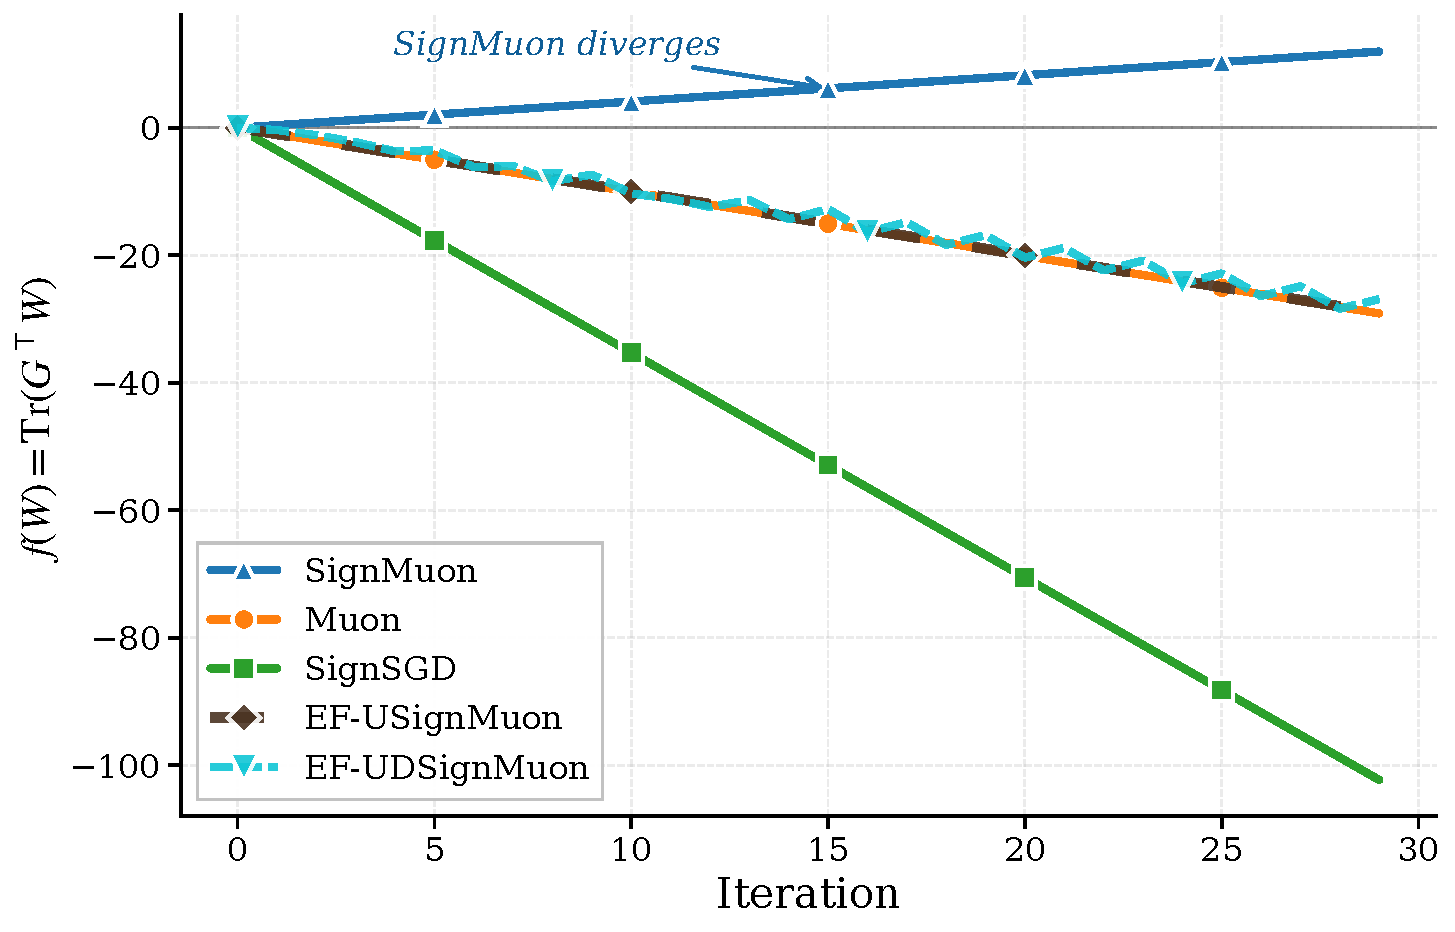
\includegraphics[width=0.9\textwidth]{images/signmuon_divergence_ef.pdf}
    \caption{Comparison of optimization trajectories for the linear objective function $f(\mathbf{W}) = \mathrm{Tr}(\mathbf{G}^\top \mathbf{W})$, demonstrating the strict divergence of SignMuon, while other methods successfully minimize the function.}
    \label{fig:divergence_plot}
\end{figure*}

We define the \textbf{USign} compressor as the directional pair $\mathrm{USign} := (\mathcal{C}_{\uparrow},\, \mathcal{C}_{\downarrow})$, where $\mathcal{C}_{\uparrow}(\mathbf{Y}) = \operatorname{mean}|\mathbf{Y}|\,\operatorname{sign}(\mathbf{Y})$ is the scaled-sign operator on the uplink (client $\to$ server) and $\mathcal{C}_{\downarrow} = I$ is the identity on the downlink
(server $\to$ client). Unlike a fully 1-bit scheme, USign compresses only the uplink to one bit per parameter, while the server broadcasts the full model. \textbf{EF21-MuonUSign} pairs USign with EF21 and the Muon LMO: the sign acts on the EF21 residual, and the optimization step uses the full Muon LMO of the reconstructed estimator.

Theorem~\ref{th:1} shows that sign-compressing the LMO direction can destroy the descent property. To restore convergence without increasing the communication volume, we replace the sign-compressed step $\mathbf{X}_{t+1}=\mathbf{X}_t -\eta_t\,\operatorname{sign}(\mathbf{D}_t)$ by an Error-Feedback variant inspired by EF21-Muon~\cite{gruntkowska2025error}.

EF21-MuonUSign maintains a gradient estimator $\mathbf{g}_t^{\mathrm{est}}$ updated via a contractive sign compressor on the residual $\Delta_t = \mathbf{M}_t - \mathbf{g}_t^{\mathrm{est}}$: 
\begin{equation}
\alpha_t = \operatorname{mean}(|\Delta_t|),\quad
\mathbf{g}_{t+1}^{\mathrm{est}} = \mathbf{g}_t^{\mathrm{est}} + \alpha_t\,\operatorname{sign}(\Delta_t),
\label{eq:ef21_central}
\end{equation}
and takes the descent step
\begin{multline}
\mathbf{X}_{t+1} = \mathbf{X}_t - \eta_t\,\,\mathbf{D}_t,
\\ \mathbf{D}_t = -A(\mathbf{g}_{t+1}^{\mathrm{est}}) \approx \mathbf{U}_{t+1}\mathbf{V}^\top_{t+1},
\label{eq:ef_step}
\end{multline}
As $\mathbf{g}_t^{\mathrm{est}}\to\mathbf{M}_t$, the direction
$\mathbf{D}_t \to \mathbf{U}_t\mathbf{V}_t^\top$ is always a descent direction,
since $\langle\nabla f,\,\mathbf{U}_t\mathbf{V}_t^\top\rangle \approx \|\nabla f\|_* > 0$.
The sign in~\eqref{eq:ef21_central} acts only on the internal compression residual, keeping the uplink at one bit per parameter. The Algorithm~\ref{central_alg_ef} is given in Appendix\ref{app:alg}. Figure~\ref{fig:divergence_plot} confirms that EF21-MuonUSign converges on the same counterexample where SignMuon diverges. We now extend this Error-Feedback mechanism to the federated setting.

While USign leaves the downlink uncompressed, a fully 1-bit scheme is obtained by compressing both channels. We define the \textbf{UDSign} compressor as the directional pair $\mathrm{UDSign}:=(\mathcal{C}_{\uparrow},\,\mathcal{C}_{\downarrow})$ with the same scaled-sign operator on both channels, $\mathcal{C}_{\uparrow}(\mathbf{Y})=\mathcal{C}_{\downarrow}(\mathbf{Y})=\operatorname{mean}|\mathbf{Y}|\,\operatorname{sign}(\mathbf{Y})$. In this version of Error Feedback Algorithm the node keeps the exact model $\mathbf{X}_t$ and takes the exact LMO step, while it observes only a compressed model shift  $\mathbf{W}_t$ reconstructed by error feedback,
\begin{multline}
  \mathbf{X}_{t+1}=\mathbf{X}_t-\eta_t\mathbf{D}_t,
\\\mathbf{W}_{t+1}=\mathbf{W}_t+\alpha_t^{\downarrow}\operatorname{sign}(\mathbf{X}_{t+1}-\mathbf{W}_t),
\end{multline}
with the gradient evaluated at $\mathbf{W}_t$ and $\mathbf{D}_t=-A(\mathbf{g}_{t+1}^{\mathrm{est}})$. The full procedure is in Algorithm~\ref{central_alg_ud}.

It should be noted that both error feedback methods require additional memory: each compressed channel maintains its own error feedback buffer (the gradient estimate $\mathbf{g}^{\mathrm{est}}$ and the model shift buffer $\mathbf{W}$ in the case of bidirectional feedback). This additional overhead is low in terms of server memory, but may be unwanted on worker nodes with limited memory.

\subsection{Federated Learning with Error Feedback}
% Алгоритм Federated SignMuon демонстрирует эмпирическую стабильность, однако знаковая компрессия неизбежно вносит смещение (bias) в направление спуска. Чтобы компенсировать ошибку квантования и обеспечить строгие гарантии сходимости, мы интегрируем в наш метод механизм Error Feedback, адаптированный для LMO-оптимизаторов в недавней работе Gruntkowska et al. \cite{gruntkowska2025error}. 
Although Federated SignMuon demonstrates strong empirical stability, sign-based compression inevitably introduces bias into the descent direction. To compensate for quantization error and ensure strong convergence guarantees, we incorporate an Error Feedback method. In the federated setting, the Error-Feedback mechanism is adapted from EF21-Muon~\cite{gruntkowska2025error}. 

% В данной модификации Federated EF21-MuonUSign процедура ортогонализации (LMO) переносится на сервер. Узлы не вычисляют LMO локально, вместо этого они вычисляют разность между текущим локальным моментумом и предыдущей оценкой градиента, после чего применяют к ней знаковую компрессию. Сервер агрегирует эти сжатые обновления, восстанавливает глобальную оценку градиента и только затем применяет к ней оператор Muon. Полный алгоритм представлен в Приложении ~\ref{app:ef21_alg}. Передача дополнительного скаляра $\alpha_t^{(j)}$ для каждого слоя практически не увеличивает размер сообщения, сохраняя общий объем трафика на уровне $\approx 1$ бита на параметр. Таким образом, обе предложенные архитектуры федеративного SignMuon: как базовая схема с мажоритарным голосованием, так и модификация с компенсацией ошибки -- успешно решают проблему коммуникационного узкого места. Они позволяют сохранить геометрические преимущества матричной ортогонализации Muon, обеспечивая при этом экстремально низкую нагрузку на сеть.
% In this Federated EF21-MuonUSign variant, the orthogonalization procedure (LMO) is moved from the clients to the server. Instead of computing the LMO direction locally, each client evaluates the difference between its current local momentum estimate and the previous gradient estimate, and then applies sign compression to this residual. The server aggregates the compressed updates, reconstructs a global gradient estimate, and only then applies the Muon operator. The complete algorithm is presented in Appendix~\ref{app:ef21_alg}. 
The LMO orthogonalization is moved from the clients to the server: each client evaluates the difference between its local momentum $\mathbf{M}_t^{(j)}$ and the previous gradient estimate $\mathbf{g}_t^{(j)}$, compresses it via scaled sign, and sends only $(\mathbf{s}_t^{(j)}, \alpha_t^{(j)})$. The server aggregates these, updates a global gradient estimator $\mathbf{G}_{t+1}$, and applies the Muon LMO. The complete Algorithm~\ref{ef21_alg} is in Appendix\ref{app:alg}. The transmission of an additional scalar $\alpha_t^{(j)}$ for each layer introduces insignificant communication overhead, keeping the uplink communication cost at $\approx 1$ bit per parameter (the server broadcasts the full model on the downlink). Thus, both federated variants -- SignMuon and EF21-MuonUSign -- effectively
address: the baseline majority-vote scheme and the error-feedback variant -- effectively address the communication bottleneck in federated learning. They preserve the geometric benefits of Muon-style matrix orthogonalization while maintaining an extremely low communication budget.

\section{Experiments}\label{sec:exp}
% Целью данных экспериментов является эмпирическая валидация алгоритма SignMuon, как оптимизатора, объединяющего высокую скорость сходимости LMO-оптимизаторов с коммуникационной эффективностью знаковой компрессии. Само исследование состоит из нескольких частей, включая валидацию в централизованном и федеративном случае, а также проверку алгоритма на синтетическом эксперименте по методу наименьших квадратов.
The goal of these experiments is empirical validation of the SignMuon and EF21-MuonUSign algorithms. The study consists of several parts, including evaluation in both centralized and federated settings, as well as validation on a synthetic least-squares optimization problem.

\subsection{Smooth Convex Optimization Problem (Synthetic Experiment)}

\begin{table*}[!t]
\centering
\footnotesize
\renewcommand{\arraystretch}{1.2}
\begin{tabular}{|l|c|c|c|}
\hline
\textbf{Algorithm} & \textbf{Learning rate ($\eta$)} & \textbf{Momentum ($\mu$)} & \textbf{Iterations to $0.001$} \\
\hline
SignMuon & 0.0002 & 0.2 & 2104 \\
Muon & 0.0065 & 0.1 & 1122 \\
EF21-MuonUSign & 0.0033 & 0.1 & 3694 \\
SignSGD & 0.00015 & 0.8 & 3120 \\
SGD & 0.1 & 0.95 & 972 \\
Adam &  0.07 & - & 202 \\
\hline
\end{tabular}
\caption{Tuned learning rates and momentum coefficients in the experiments on the smooth convex optimization problem (Equation~\ref{eq:synthetic_problem}).}
\label{tab:synthetic_results}
\end{table*}

% Для того чтобы оценить влияние матричной структуры на ход оптимизации (без влияния стохастического шума и сложной архитектуры нейронных сетей), мы начинаем эксперименты с детерминированной $L-$гладкой выпуклой задачи. Для этого рассмотрим задачу минимизации квадратичной формы:
To evaluate the effect of matrix structure on the optimization process (without the influence of stochastic noise or the complexity of DNN architectures), we begin our experiments with a deterministic $L$-smooth convex optimization problem. We consider the minimization of a quadratic form:
\begin{multline}
F(\mathbf{X}) = \frac{1}{2} \|\mathbf{A}^{1/2} \mathbf{X} \mathbf{B}^{1/2}\|_F^2 \\
= \frac{1}{2} \langle \mathbf{X}, \mathbf{A} \mathbf{X} \mathbf{B} \rangle \to \min_{\mathbf{X} \in \mathbb{R}^{m \times n}},
\label{eq:synthetic_problem}
\end{multline}
where the parameter matrix $\mathbf{X} \in \mathbb{R}^{m \times n}$ has dimension $m = n = 500$, which is representative of the size of parameter matrices in deep neural networks. The matrices $\mathbf{A} \in \mathbb{S}_+^m$ and $\mathbf{B} \in \mathbb{S}_+^n$ are symmetric positive semidefinite. To generate the problem instance, we randomly construct the spectra of $\mathbf{A}$ and $\mathbf{B}$ by sampling their eigenvalues uniformly from the interval $(0, 1)$, which guarantees a smoothness constant $L \le 1$ with respect to the Frobenius norm. The parameter matrix $\mathbf{X}_0$ is initialized with elements sampled independently from a normal distribution $\mathcal{N}(0, 0.01)$.

% Поскольку теоретические оценки скорости сходимости зависят от выбора нормы и констант гладкости, будем использовать эмпирический критерий эффективности: алгоритмы оцениваются по минимальному количеству итераций, необходимых для достижения порогового значения функции потерь $F(\mathbf{X}) \le 0.001$, максимальное число итераций $T_{\max} = 5000$. Для поиска оптимальных гиперпараметров оптимизаторов был проведен сеточный поиск (Grid Search) по learning rate $\eta$ и коэффициенту моментума $\mu$ для каждого из пяти рассматриваемых оптимизаторов:
Since theoretical convergence guarantees depend on the choice of norm and the corresponding smoothness constants, we adopt an empirical evaluation criterion. Specifically, the optimizers are compared by the minimum number of iterations required to reach the target function $F(\mathbf{X}) \le 0.001$, with a maximum number of iterations set to $T_{\max} = 5000$.  We perform a grid search over the hyperparameter ranges for each of the optimization algorithms under consideration (Table~\ref{tab:grid_search}).
% \begin{itemize}
%     \item $\mu \in \{0.1, 0.2, 0.3, 0.4, 0.5, 0.6, 0.7, 0.8, 0.9, 0.95\}$ для всех алгоритмов, кроме Adam;
%     \item $\eta \in [0.005, 0.020]$ с шагом $0.001$ для Muon;
%     \item $\eta \in [1\cdot 10^{-4}, 0.001]$ с шагом $10^{-4}$ для SignMuon;
%     \item $\eta \in [5\cdot 10^{-5}, 2\cdot 10^{-4}]$ с шагом $10^{-5}$ для SignSGD;
%     \item $\eta \in [0.01, 0.10]$ с шагом $0.01$ для SGD и Adam.
% \end{itemize}

The results of the grid search with the number of iterations required to converge to 0.001, are summarized in Table~\ref{tab:synthetic_results}. Muon converges in 1122 iterations, comparable to SGD (972) but slower than Adam (202). SignMuon reaches the target in 2104 iterations, significantly outperforming SignSGD (3120). EF21-MuonUSign requires 3694 iterations; its overhead on this benign convex problem is expected, since its purpose is to guarantee convergence on problems where SignMuon does not converge (Theorem~\ref{th:1}). The optimization trajectories are shown in Appendix\ref{app:images_task}, Figure~\ref{fig:synthetic_results}.

% Из результатов видно, что алгоритм Muon достиг оптимума за 1122 итерации, что сопоставимо с классическими методами первого порядка (Adam, SGD). Стоит отметить, что алгоритм SignMuon достигает целевого значения функции потерь за 2104 итерации, значительно превосходя базовый алгоритм SignSGD (3120 итераций). Динамика целевой функции и нормы градиента в процессе оптимизации проиллюстрированы в Приложении на Рисунке \ref{fig:synthetic_results}.

\subsection{Centralized Learning}
\begin{figure*}[!t]
    \begin{subfigure}[b]{0.48\textwidth}
        \centering
        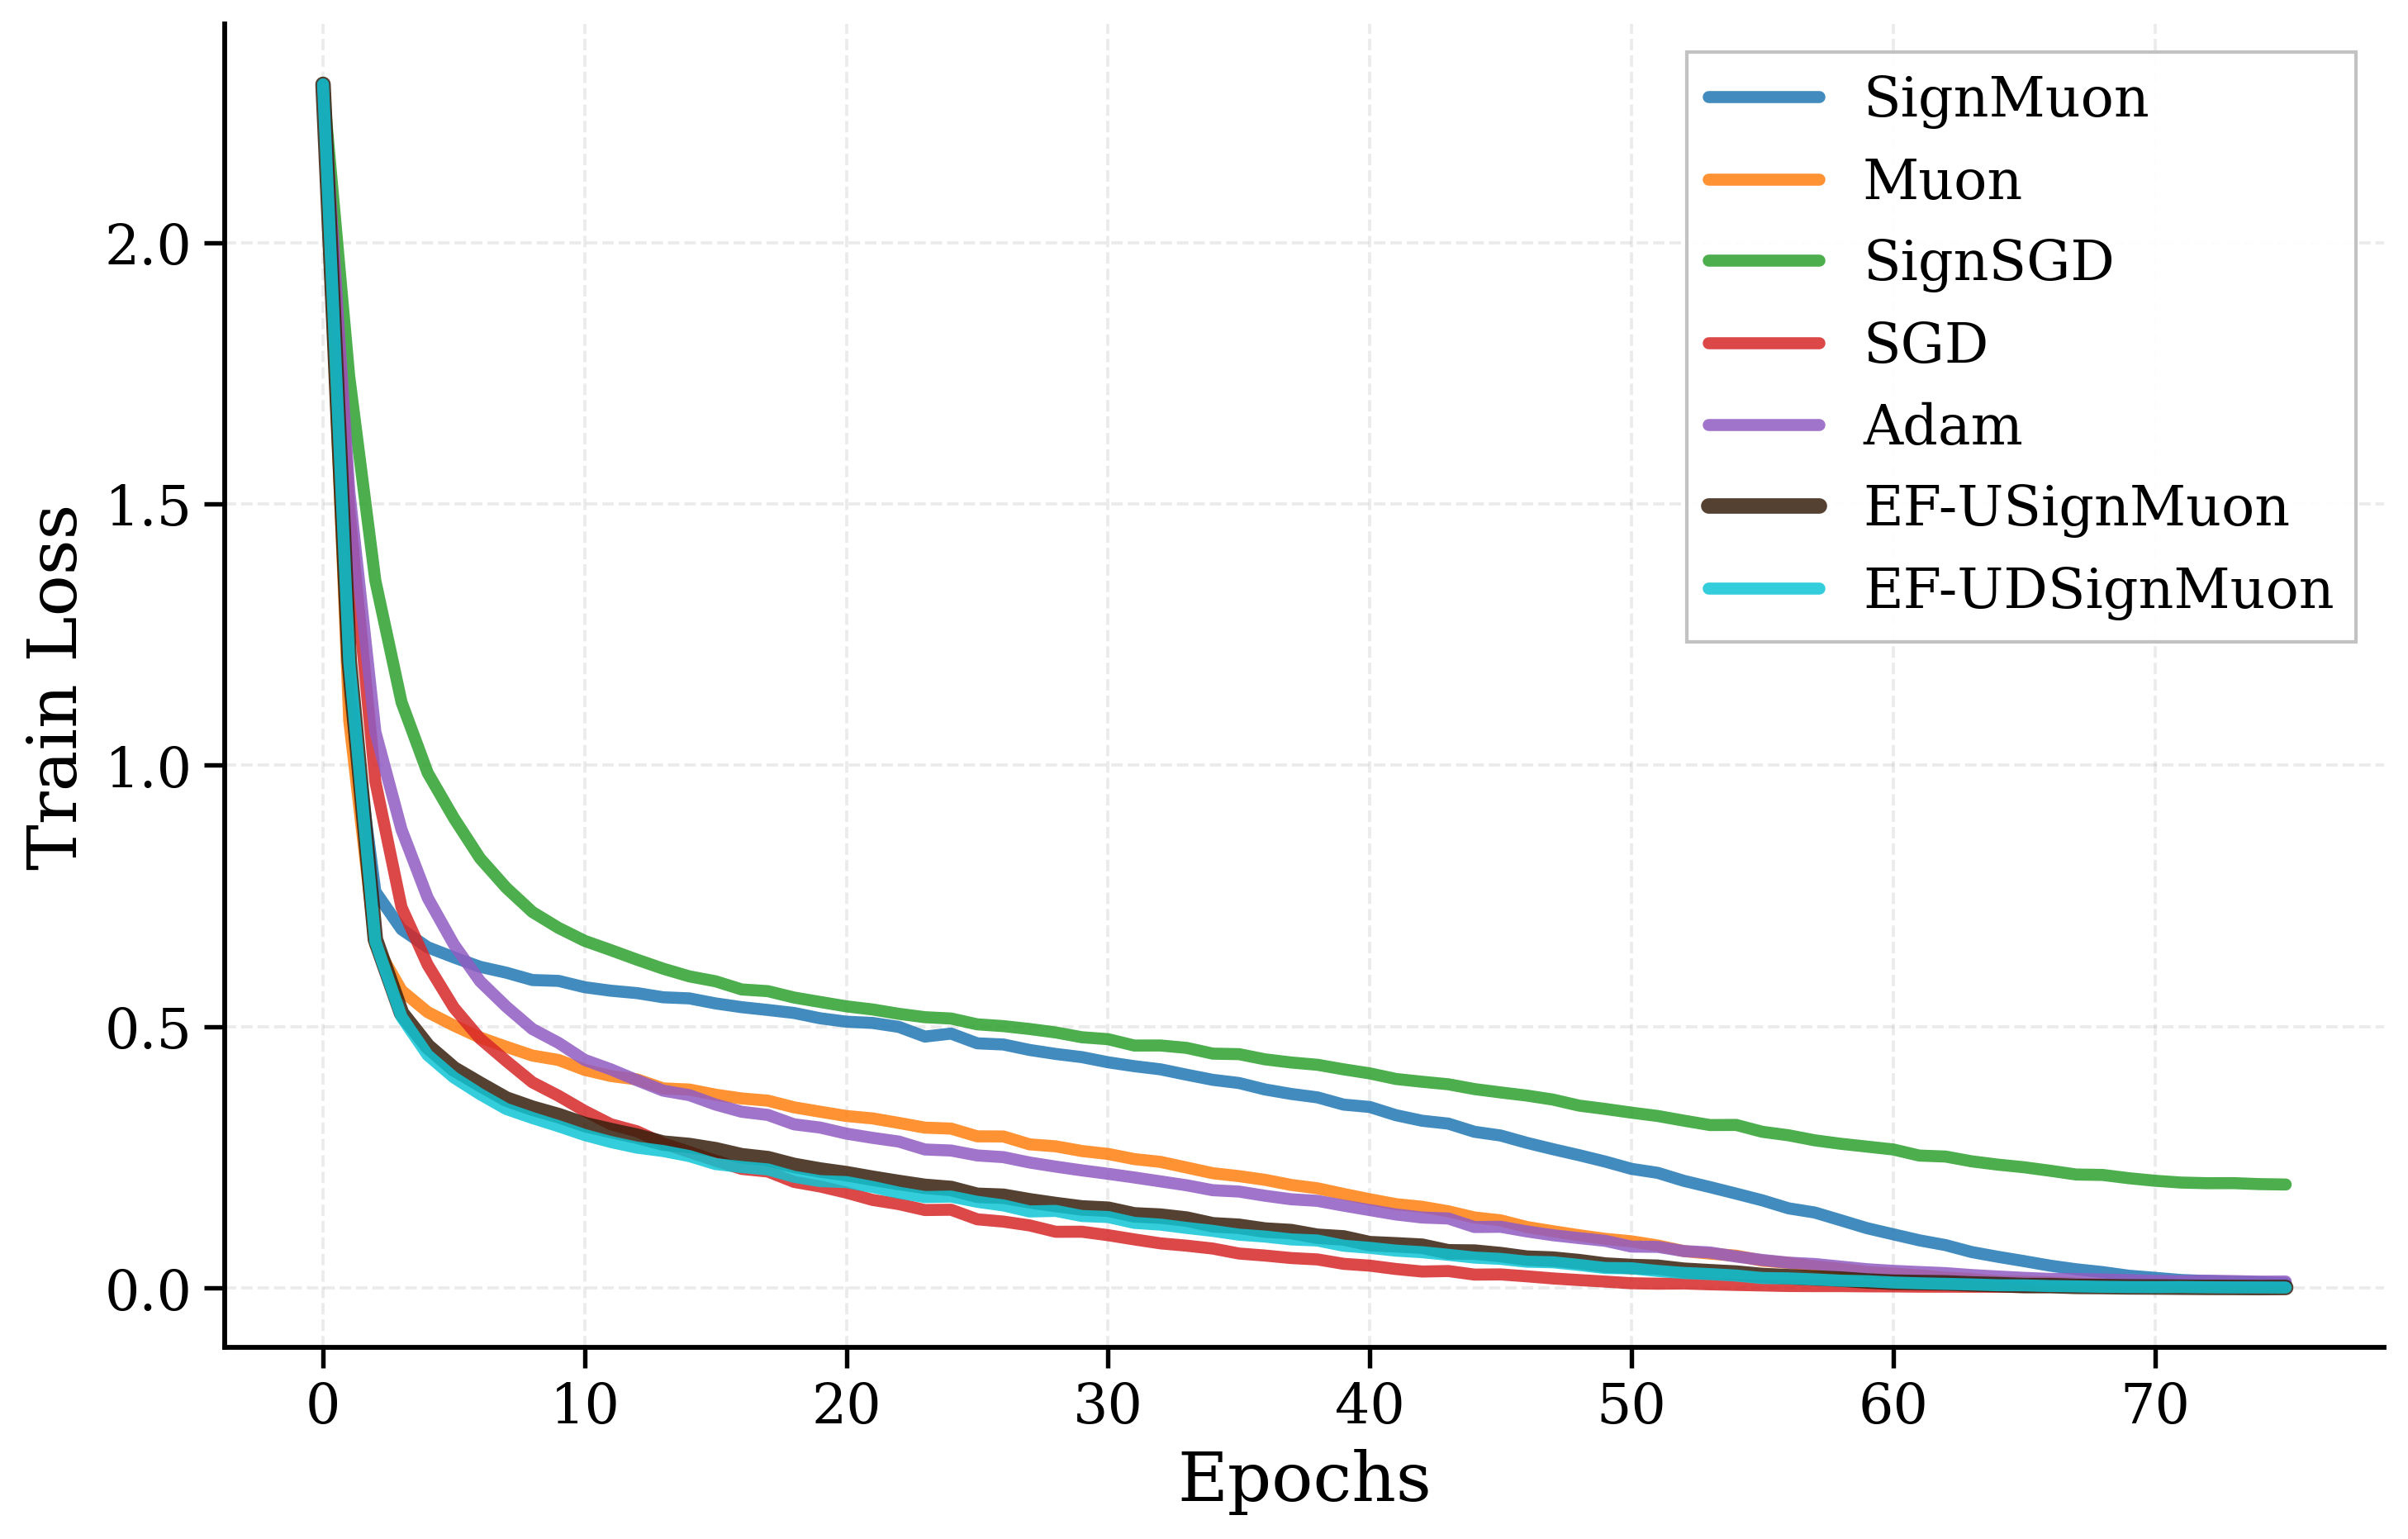
\includegraphics[width=\textwidth]{images/centralized_images/train_loss_resnet.png}
        \caption{Train Loss}
    \end{subfigure}
    \hfill
    \begin{subfigure}[b]{0.48\textwidth}
        \centering
        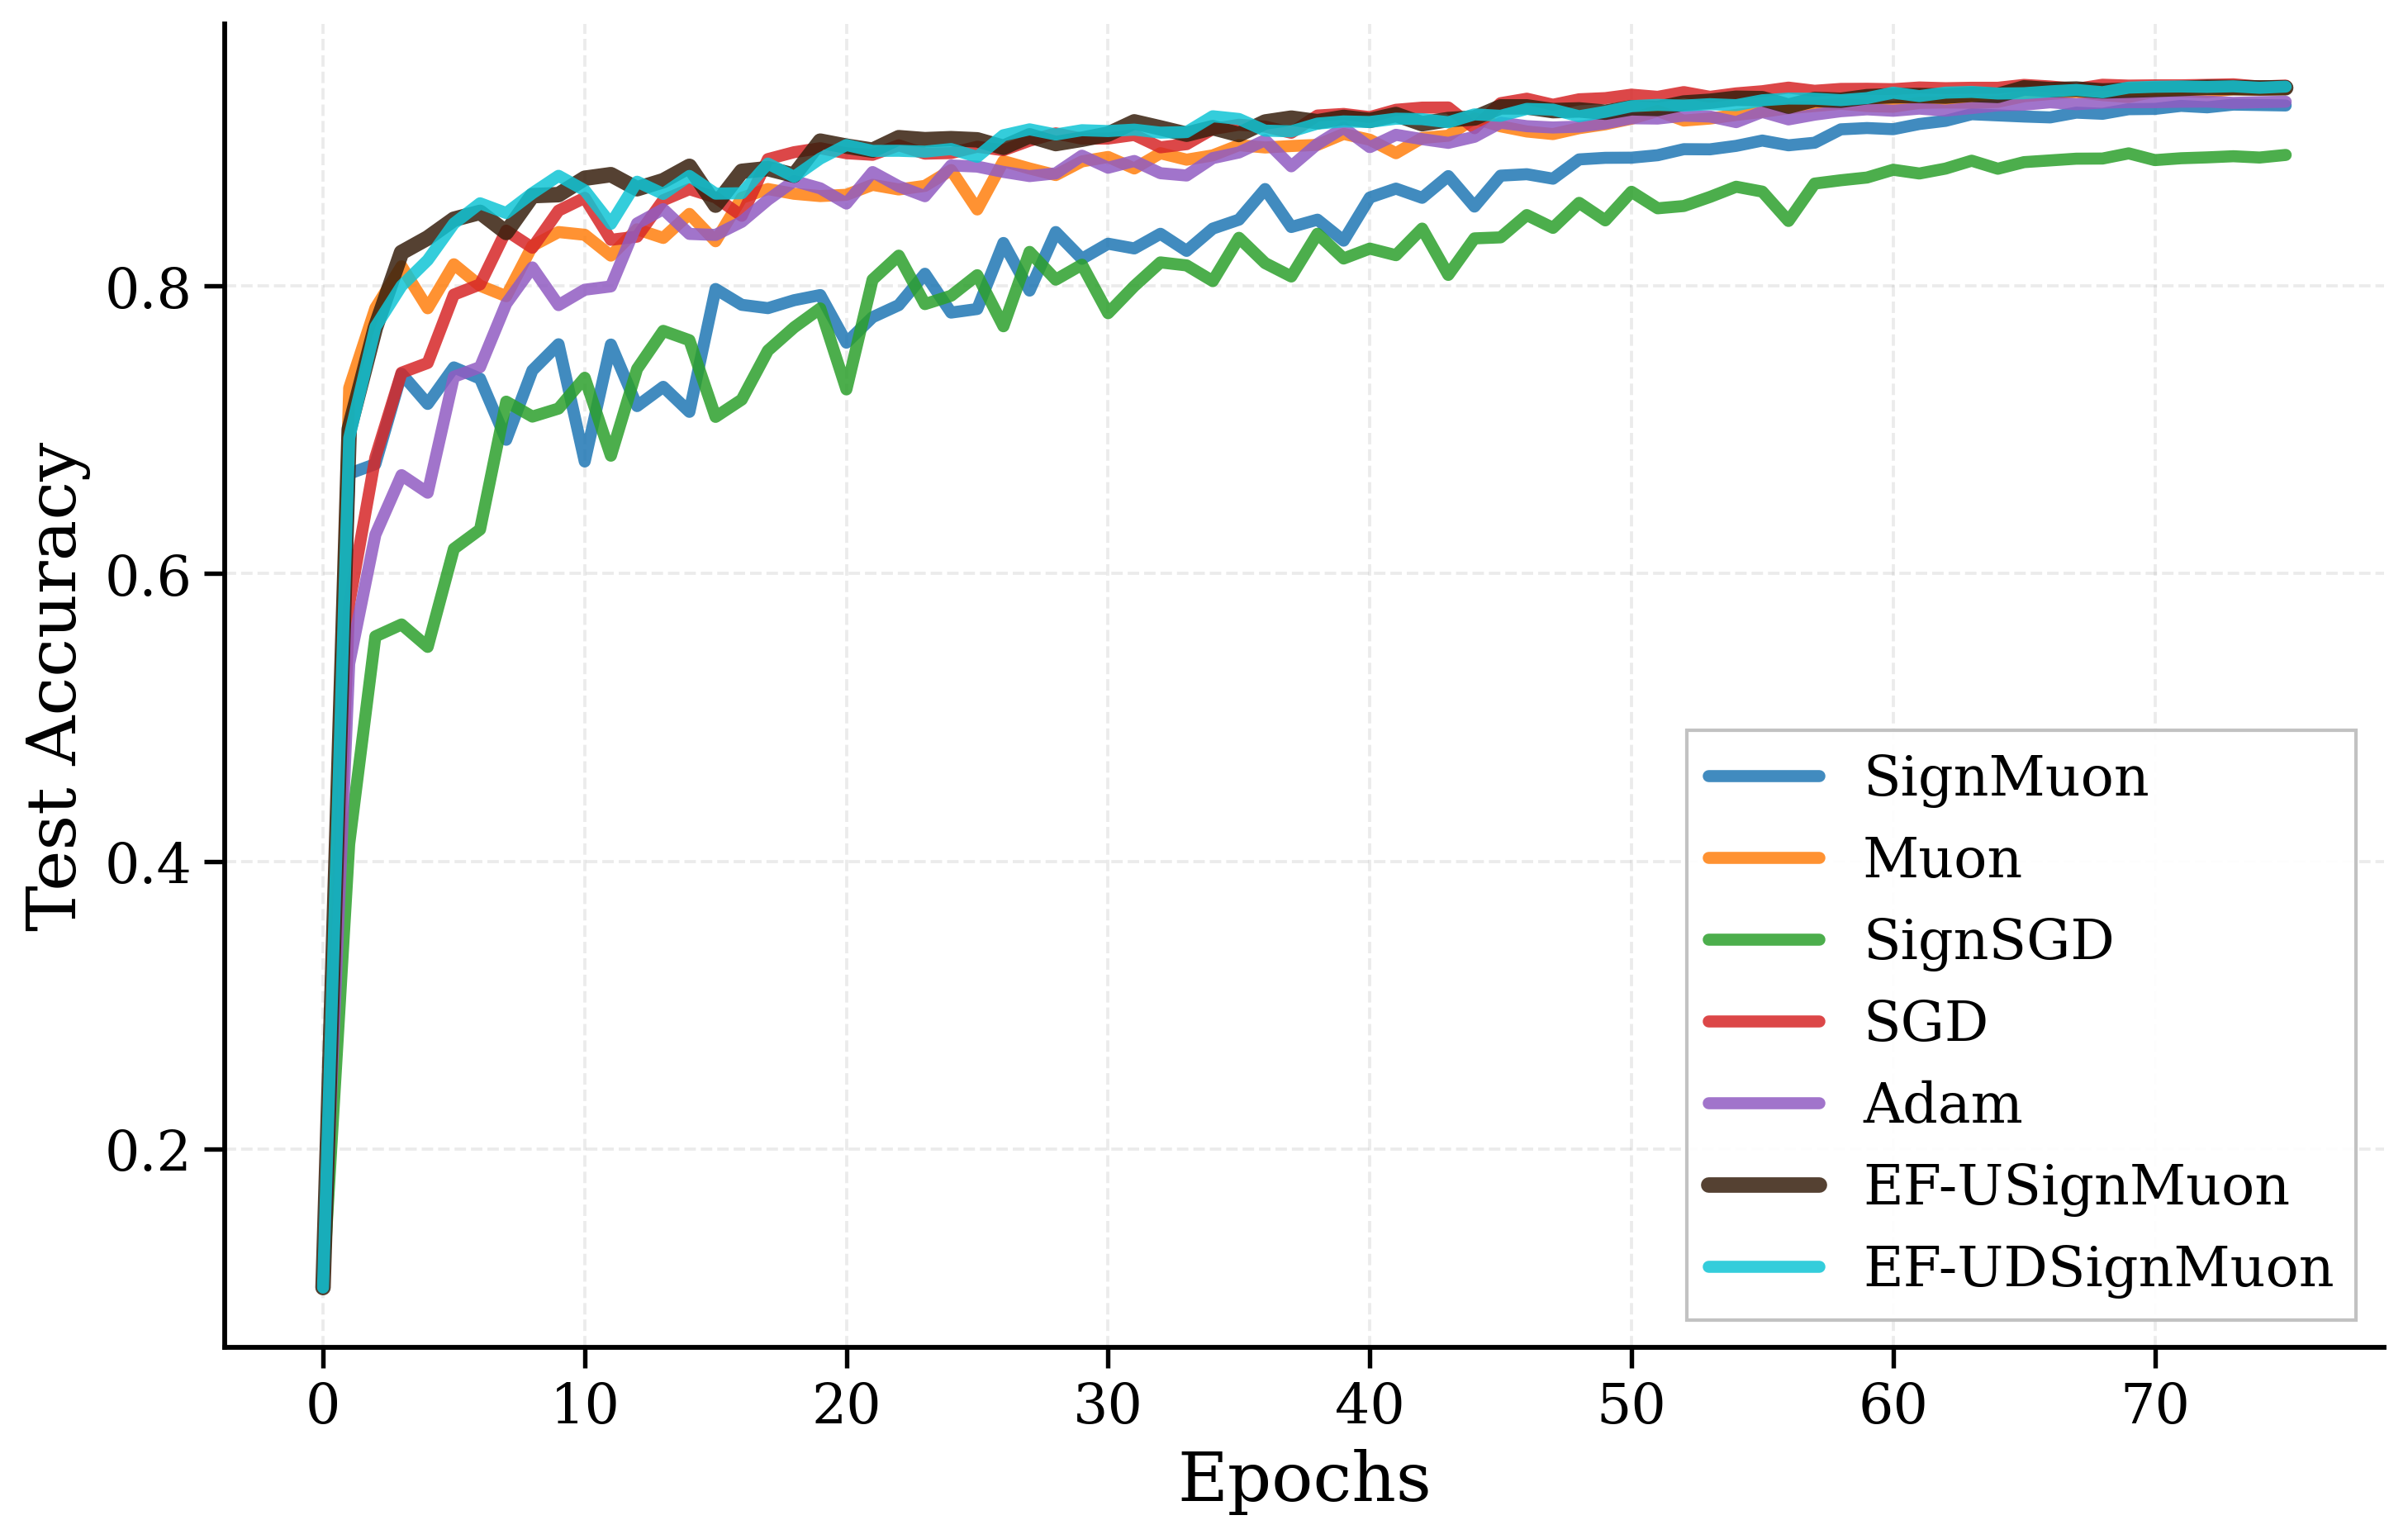
\includegraphics[width=\textwidth]{images/centralized_images/test_acc_resnet.png}
        \caption{Test Accuracy}
    \end{subfigure}
    \caption{Centralized setting. Comparison of convergence and classification accuracy achieved by different optimization algorithms while training a ResNet-18 classifier on CIFAR-10.}
    \label{fig:cifar_results}
\end{figure*}

% В данном эксперименте мы сравниваем динамики сходимости и итоговые точности (Accuracy) алгоритма SignMuon с классическими оптимизаторами Muon, SignSGD, SGD и Adam при фиксированном количестве эпох. Одной из задач эксперимента является демонстрация того, что SignMuon обеспечивает высокое качество классификации, сопоставимое с Muon, при этом превосходит по точности классический алгоритм SignSGD при идентичной коммуникации (1 бит на параметр).  
In this experiment, we compare the convergence dynamics and the final accuracies of SignMuon and EF21-MuonUSign with those of the classical optimizers: Muon, SignSGD, SGD, and Adam at a fixed number of epochs. One of the goals of the experiment is to demonstrate that SignMuon achieves classification quality comparable to Muon, while outperforming the classical SignSGD algorithm under the same uplink communication budget (1 bit per parameter on the uplink).


% Эксперименты проводились на датасетах MNIST и CIFAR-10:
% \begin{itemize}
%     \item \textbf{CIFAR-10:} Стандартный датасет для задачи классификации изображений. Содержит 60 000 цветных изображений 10 классов. Каждое изображение представлено в виде тензора размерности $3 \times 32 \times 32$, где первый индекс соответствует количеству цветовых каналов (RGB). Для централизованного обучения датасет делится на обучающую и тестовую выборки. В федеративном сценарии обучающая выборка делится между узлами.
%     \item \textbf{MNIST:} Датасет для задачи классификации изображений, используемый в бенчмарках распределенного обучения. Содержит 70 000 черно-белых изображений рукописных цифр (10 классов, по классу на каждую цифру) размером $28 \times 28$ пикселей (1 канал). Как и в случае с CIFAR-10, для централизованного обучения датасет делится на обучающую и тестовую выборки, а для федеративного сценария обучающая выборка делится между узлами.
% \end{itemize}

The experiments are conducted on CIFAR-10. It is a standard image classification dataset. It contains 60{,}000 color images of 10 classes. Each image is represented as a tensor of size $3 \times 32 \times 32$, where the first dimension corresponds to the number of color channels (RGB). For centralized training, the dataset is split into training and test sets. In federated learning, the training set is partitioned across the clients.
% Эксперименты проводились на датасете CIFAR-10: стандартный датасет для задачи классификации изображений. Содержит 60 000 цветных изображений 10 классов. Каждое изображение представлено в виде тензора размерности $3 \times 32 \times 32$, где первый индекс соответствует количеству цветовых каналов (RGB). Для централизованного обучения датасет делится на обучающую и тестовую выборки. В федеративном сценарии обучающая выборка делится между узлами.

The base model is a ResNet-18 architecture adapted to low-resolution images by using an initial $3\times3$ convolution without max-pooling. The network consists of 4 residual blocks with Batch Normalization (BatchNorm), followed by a dropout regularization layer and a linear classifier. As mentioned above, training is run for a fixed number of epochs $T_{\max}=75$. During training, the learning rate is annealed with a cosine scheduler (CosineAnnealingLR). The learning rate $\eta_t$ at epoch $t$ is updated as follows:
% В качестве базовой модели была использована архитектура ResNet-18, адаптированная под изображения малого разрешения за счет использования начальной свертки $3\times3$ без макс-пулинга. Сеть включает четыре блока остаточных слоев (Residual Blocks) с пакетной нормализацией (BatchNorm), завершаясь слоем регуляризации Dropout и линейным классификатором. Как было сказано ранее обучение происходило при фиксированном количестве эпох $T_{max}=75$. В процессе обучения learning rate варьируется, используя косинусный планировщик скорости обучения (CosineAnnealingLR). Обновление learning rate $\eta_t$ на эпохе $t$ осуществляется по следующей формуле:
\begin{equation}
\eta_t = \eta_{\text{min}} + \frac{1}{2}(\eta_{\text{max}} - \eta_{\text{min}})\left(1 + \cos\left(\frac{t}{T_{\text{max}}}\pi\right)\right),
\end{equation}
where $\eta_{\text{max}}$ is the initial learning rate of the algorithm, $\eta_{\text{min}} = 0$ is the minimum value (in our configuration), and $T_{\text{max}}$ is the total number of training epochs.
% Результаты эксперимента и значения подобранных гиперпараметров указаны в Таблице \ref{tab:cifar_central}. Динамика целевой функции и точности алгоритмов в процессе обучения проиллюстрированы в Приложении~\ref{app:images_cen}.

The experimental results and the selected hyperparameter values are reported in Appendix in Table~\ref{tab:cifar_central}. The dynamics of the loss function and of the accuracy of the algorithms during training are illustrated in Figure~\ref{fig:cifar_results}. Notably, EF21-MuonUSign achieves $93.82\%$ test accuracy, surpassing SignMuon ($92.55\%$) and matching Muon ($93.70\%$), confirming that the Error-Feedback mechanism does not sacrifice practical accuracy.

\subsection{Federated Learning}
\begin{table*}[!t]
\centering
\small
\renewcommand{\arraystretch}{1.2}
\begin{tabular}{|c|c|c|c|c|c|c|c|c|}
\hline
\textbf{Dataset} & \textbf{Optimizer} & \textbf{Rounds} & \textbf{Clients} & \textbf{Steps} & \textbf{Batch} & \textbf{LR} & \textbf{Mom} & \textbf{Test Acc} \\
\hline
\multirow{6}{*}{CIFAR-10} & SignMuon & \multirow{6}{*}{2000} & \multirow{6}{*}{10} & \multirow{6}{*}{3} & \multirow{6}{*}{64} & 0.001 & \multirow{6}{*}{0.9} & 84.57\% \\
\cline{2-2} \cline{7-7} \cline{9-9}
 & Muon & & & & & 0.05 & & 85.22\% \\
\cline{2-2} \cline{7-7} \cline{9-9}
 & SignSGD & & & & & 0.001 & & 78.98\% \\
\cline{2-2} \cline{7-7} \cline{9-9}
 & SGD & & & & & 0.03 & & 81.38\% \\
\cline{2-2} \cline{7-7} \cline{9-9}
 & Adam & & & & & 0.001 & & 78.36\% \\
\cline{2-2} \cline{7-7} \cline{9-9}
 & EF21-MuonUSign & & & & & 0.02 & & 84.59\% \\
\hline
\end{tabular}
\caption{CIFAR-10: federated learning. Experiment~3: Comparison of the algorithms with $N=10$ clients.}
\label{tab:exp_3}
\end{table*}

The next stage of the research was adaptation of SignMuon in federated learning, where transmitting full 32-bit gradient matrices is the communication bottleneck. The goal of this stage is to confirm that extreme compression of the orthogonalized updates attains an accuracy comparable to that of Muon, while significantly reducing the volume of transmitted data.
% Следующим этапом исследования стала оценка эффективности SignMuon в сценарии федеративного обучения (Federated Learning), где передача полных 32-битных матриц градиентов является узким местом. Цель экспериментов данного этапа -- подтвердить, что экстремальное сжатие ортогонализованных обновлений позволяет достичь точности, сопоставимой с алгоритмом Muon, при экстремальном снижении объема передаваемой информации.


For these experiments, we implemented a federated architecture with a central aggregation server. To keep the results comparable with the previous stages, we used the convolutional neural network (CNN2), comprising two convolutional blocks with BatchNorm and an MLP classifier. The CIFAR-10 dataset was partitioned across the clients homogeneously (homogeneous split). Within this learning type, we study both the baseline Federated SignMuon scheme (Algorithm~\ref{fed_alg}) and the error-feedback variant Federated EF21-MuonUSign (Algorithm~\ref{ef21_alg}). Each communication round consists of a local gradient accumulation step on the clients, followed by transmitting the sign-compressed updates to the server, which updates the global model.
% Для проведения тестов была реализована федеративная архитектура с центральным сервером агрегации. Чтобы обеспечить сопоставимость результатов с предыдущими этапами работы, использовалась та же сверточная нейронная сеть (CNN2), включающая два сверточных блока с BatchNorm и MLP-классификатор. Набор данных CIFAR-10 подвергался однородному (\textit{homogeneous}) разбиению между узлами. В рамках данного сценария мы исследовали как базовую схему Federated SignMuon (\cref{fed_alg}), так и модификацию с механизмом учета ошибки Federated EF21-MuonUSign (\cref{ef21_alg}). Каждый раунд обучения включал этап локального накопления градиента на узлах с последующей передачей данных, прошедших знаковую компрессию, на сервер для обновления глобальной модели.


For a systematic analysis of the proposed algorithms, this experimental stage is split into several sub-experiments. First, we assess how the scale of the federated network affects the stability of sign-based optimization and the final accuracy of the model. To this end, we study the baseline SignMuon algorithm for different numbers of active clients.
% Для системного анализа свойств предложенных алгоритмов данный этап экспериментального исследования был разделен на несколько подэкспериметов. В первую очередь необходимо было оценить, как масштаб федеративной сети влияет на стабильность знаковой оптимизации и итоговую точность модели. С этой целью было проведено детальное изучение базового алгоритма SignMuon при различном количестве активных узлов в системе

\textbf{Experiment~1: Scalability of SignMuon with respect to the number of clients.} 
% Исследовалась зависимость числа участвующих узлов на качество обучения с алгоритмом SignMuon. Число узлов $N \in [1, 3, 5, 7, 9]$ при 2000 раундах обучения и одном локальном шаге на узле. Результаты показали рост точности классификации с увеличением числа узлов. Данный эффект объясняется улучшением качества агрегации через majority vote при большем числе независимых оценок знака градиента. Результаты данного эксперимента приведены в Приложении ~\ref{app:results_fed:1}. 
We investigate the effect of the number of participating clients on the training quality of SignMuon. The number of clients is $N \in \{1, 3, 5, 7, 9\}$, with 2000 training rounds and one local step per client. The results show that classification accuracy grows with the number of clients. This effect is explained by the improved quality of majority-vote aggregation as more independent sign estimates of the gradient become available. The results of this experiment are reported in Appendix\ref{app:results_fed:1}.

Having confirmed the positive effect of the number of clients on the stability of the algorithm, we proceed to a direct comparison of SignMuon with the existing algorithms. For this purpose, we select a configuration with 3 clients, which allows us to evaluate the efficiency of the algorithms under limited federation resources.
% Подтвердив положительное влияние количества узлов на стабильность алгоритма, мы перешли к прямому сравнению SignMuon с существующими алгоритмами. Для этого была выбрана конфигурация из трех узлов, позволяющая оценить эффективность алгоритмов в условиях ограниченных ресурсов федерации.

\textbf{Experiment~2: Comparison of the algorithms with $N=3$ clients.} We compare 6 optimizers with 3 clients, 2000 rounds, and 1 local step. The results of this experiment are reported in Appendix\ref{app:results_fed:2}.

However, the potential of sign-based optimization algorithms is most fully revealed when the scale of the network and the amount of local computation increase. Therefore, at the final testing stage we increased the number of clients to 10.

\textbf{Experiment~3: Comparison of the algorithms with $N=10$ clients.} 
% Те же шесть оптимизаторов тестировались в условиях 10 узлов, 2000 раундов и трех локальных шагов на узле. В данном режиме SignMuon достиг качества Muon. Вывод эксперимента: при достаточном числе узлов ($N \geq 10$) алгоритм SignMuon обеспечивает качество, сопоставимое с Muon, при этом сокращая объем передаваемых данных в $\sim$32 раза за счет передачи только знаков градиентов вместо полных значений. Результаты данного эксперимента приведены в Таблице \ref{tab:exp_3}, а также на Рисунке \ref{fig:exp_3}. 
The same 6 optimizers are tested with 10 clients, 2000 rounds, and 3 local steps per client. In this learning type, SignMuon reaches the quality of Muon. We conclude that, with a sufficient number of clients ($N \ge 10$), SignMuon achieves a quality comparable to Muon while reducing the volume of transmitted data by a factor of ${\sim}32\times$, by transmitting only the signs of the gradients instead of their full values. The results of this experiment are reported in Table~\ref{tab:exp_3} and Figure~\ref{fig:exp_3}. EF21-MuonUSign ($84.59\%$) performs on par with SignMuon ($84.57\%$), demonstrating that the convergence guarantee comes at no accuracy cost in the federated setting.




\section{Conclusion}\label{sec:conclusion}
% В данной работе был предложен алгоритм SignMuon -- метод оптимизации на основе LMO, который объединяет структурные преимущества матричной ортогонализации с экстремальной знаковой компрессией для коммуникационной эффективности. Наш подход объединил принципы работы современных оптимизаторов, таких как Muon, и семейство алгоритмов SignA, обеспечивая снижение объема передаваемых данных в 32 раза. Мы разработали аналитическую базу для исследования сходимости SignMuon на гладкой выпуклой задаче. В данном этапе исследования мы убедились, что LMO-обновление сохраняет свои геометрические преимущества даже после 1-битного сжатия (SignMuon значительно превосходит SignSGD в скорости сходимости до целевой точности по итерациям). Экспериментальные результаты на наборах данных MNIST и CIFAR-10, а также в сценариях федеративного обучения подтверждают практическую применимость предложенного метода: SignMuon демонстрирует точность, сопоставимую с алгоритмом Muon, и существенно превосходит классический SignSGD.

% Несмотря на то, что данная работа предлагает новый комбинированный алгоритм, она также подсвечивает новые направления для будущих исследований. Наш анализ в рамках \cref{th:1} выявил ограничение: в отличие от стандартного градиентного спуска, сочетание LMO и знаковой компрессии может приводить к расходимости в специфических условиях доминирующего сингулярного шума. Кроме того, наши текущие теоретические гарантии опираются на предположение о точном вычислении LMO-направления, в то время как на практике используются полиномиальные приближения с помощью метода Ньютона-Шульца. 

% Таким образом, мы добились существенных результатов в построении структурированного и коммуникационно-эффективного алгоритма оптимизации. Тем не менее, данная область остается открытой, оставляя множество путей для будущих исследований.

This work proposes SignMuon, which applies 1-bit sign compression to the Muon LMO direction to bridge structured optimization and extreme communication efficiency in federated learning. While it empirically matches Muon's accuracy and outperforms SignSGD, we formally prove that direct sign-compressed LMO lacks global convergence guarantees and can diverge. To resolve this without compromising uplink efficiency, we introduce EF21-MuonUSign, an Error-Feedback variant that applies sign compression to the internal residual rather than the LMO step. EF21-MuonUSign restores convergence on our counterexample and achieves Muon-level performance while maintaining a 1-bit uplink. Our framework establishes a foundation for adapting matrix-aware optimizers to bandwidth-constrained distributed training without sacrificing model accuracy.
\paragraph{Future work.} An extension of EF21-MuonUSign is a bidirectional scheme that compresses both the uplink (client $\to$ server) and the downlink (server $\to$ client), in the spirit of the two-sided framework of \citet{gruntkowska2025error}. In this work we focus on uplink compression, since the aggregation of many client messages is typically the dominant communication bottleneck, and we keep the downlink at full precision ($\mathcal{C}_{\downarrow} = I$). Furthermore, investigating how these matrix-aware 1-bit strategies scale to the massive parameter matrices of Large Language Models is a highly promising direction for future research.





%%%%%%%%%%%%%%%%%%%%%%%%%%%%%%%%%%%%%%%%%%%%%%%%%%%%%%%%%%%%

% \newpage
% References moved to the end of the document (after the Appendix): with four
% two-column floats in the main text, the bibliography otherwise starts on the
% same page as Table 2. Placing it last lets every two-column float land before
% the references.
% \bibliographystyle{unsrtnat}  % aaai2027.sty sets the style to aaai2027.bst automatically
% \bibliography{references}

%%%%%%%%%%%%%%%%%%%%%%%%%%%%%%%%%%%%%%%%%%%%%%%%%%%%%%%%%%%%

%\newpage
\appendix 
\section{Appendix}\label{app}
% \subsection{Additional experiments / Proofs of Theorems}\label{app:exp}
\subsection{Proof of Theorem~\ref{th:1} (Divergence of SignMuon)}\label{app:proof_th1}

\paragraph{Proof} TODO: add momentum support. The proof is constructed using a counterexample that shows the existence of a smooth function and a matrix dimension $N_{dim} \ge 4$ for which the SignMuon algorithm is guaranteed to diverge. We conjecture, supported by extensive numerical search, that no such counterexample exists for $N_{dim}\le3$. However, at $N_{dim} = 4$, this convergence guarantee vanishes.

Consider a simple linear objective function $f(\mathbf{W}) = \mathrm{Tr}(\mathbf{G}^\top \mathbf{W})$. For standard gradient descent or Muon, such a function diverges towards $-\infty$. The gradient is globally constant: $\nabla f(\mathbf{W}_t) = \mathbf{G}$ for all $t$. The change in the objective function at each iteration of the SignMuon algorithm is given by:
\begin{equation}
f(\mathbf{W}_{t+1}) - f(\mathbf{W}_t) = -\eta \langle \mathbf{G}, \operatorname{sign}(\mathbf{U} \mathbf{V}^\top) \rangle.
\end{equation} 
To prove divergence, it is sufficient to present a matrix $\mathbf{G}$ for which $\langle \mathbf{G}, \operatorname{sign}(\mathbf{U} \mathbf{V}^\top) \rangle < 0$. In this case, $f(\mathbf{W})$ strictly increases at every step, and the algorithm perpetually moves in the wrong direction.

We construct $\mathbf{G} \in \mathbb{R}^{4 \times 4}$ by defining a specific orthogonal matrix $\mathbf{O}$ and a specific rank-1 principal component $\mathbf{u}_1 \mathbf{v}_1^\top$. Let the orthogonal matrix $\mathbf{O}$ be given by the following exact rational numbers:
\begin{equation}
\mathbf{O} = \frac{1}{103} \begin{pmatrix} 101 & 20 & 2 & -2 \\ -20 & 97 & 20 & -20 \\ -2 & 20 & 2 & 101 \\ -2 & 20 & -101 & -2 \end{pmatrix}.
\end{equation}
Because no entry is zero, its element-wise sign matrix $\mathbf{S} = \operatorname{sign}(\mathbf{O})$ is uniquely defined. Now, let $\mathbf{u}_1$ and $\mathbf{v}_1$ be the following exact unit vectors:
\begin{equation}
\mathbf{u}_1 = \frac{1}{\sqrt{309}} \begin{pmatrix} 10 \\ -3 \\ 10 \\ 10 \end{pmatrix}, \quad \mathbf{v}_1 = \frac{1}{\sqrt{309}} \begin{pmatrix} 10 \\ 3 \\ -10 \\ 10 \end{pmatrix}.
\end{equation}
One can easily verify that $\mathbf{O} \mathbf{v}_1 = \mathbf{u}_1$, meaning $\mathbf{u}_1$ and $\mathbf{v}_1$ act perfectly as left and right singular vectors for this orthogonal space. The crucial feature of this geometry is that the Frobenius inner product between this rank-1 component and the sign matrix $\mathbf{S}$ yields an exact, strictly negative fraction:
\begin{equation}
\langle \mathbf{u}_1 \mathbf{v}_1^\top, \mathbf{S} \rangle = \mathbf{u}_1^\top \mathbf{S} \mathbf{v}_1 = -\frac{43}{103}.
\end{equation}

We construct the gradient matrix $\mathbf{G}$ by assigning a massive singular value ($\sigma_1 = 1001$) to this pathological component and a singular value of $1$ to the rest of the orthogonal space:
\begin{equation}
    \mathbf{G} \approx \begin{pmatrix}
        324.6 & 97.3 & -323.6 & 323.6 \\
        -97.3 & -28.2 & 97.3 & -97.3 \\
        323.6 & 97.3 & -323.6 & 324.6 \\
        323.6 & 97.3 & -324.6 & 323.6 \\
      \end{pmatrix}.
\end{equation}
% By definition of the Singular Value Decomposition (SVD), the leading singular vectors of $\mathbf{G}$ are $\mathbf{u}_1$ and $\mathbf{v}_1$ (with $\sigma_1 = 1001$), and the remaining singular values are $\sigma_2 = \sigma_3 = \sigma_4 = 1$. Consequently, the Muon orthogonalized step is exactly identical to $\mathbf{O}$, i.e., $\mathbf{U}_G \mathbf{V}_G^\top = \mathbf{O}$.
Indeed, since $\mathbf{G}=1000\,\mathbf{u}_1\mathbf{v}_1^\top+\mathbf{O}$ and $\mathbf{O}\mathbf{v}_1=\mathbf{u}_1$,
\[
\mathbf{G}\mathbf{v}_1 = 1000\,\mathbf{u}_1(\mathbf{v}_1^\top\mathbf{v}_1)+\mathbf{O}\mathbf{v}_1 = 1001\,\mathbf{u}_1,
\]
so $(\mathbf{u}_1,\mathbf{v}_1)$ is a singular pair of $\mathbf{G}$ with $\sigma_1=1001$. For any $\mathbf{w}\perp\mathbf{v}_1$ we have
$\mathbf{G}\mathbf{w}=\mathbf{O}\mathbf{w}$; as $\mathbf{O}$ is orthogonal and $\mathbf{O}\mathbf{v}_1=\mathbf{u}_1$, the restriction
$\mathbf{O}|_{\mathbf{v}_1^\perp}$ is an isometry onto $\mathbf{u}_1^\perp$, hence $\sigma_2=\sigma_3=\sigma_4=1$. Moreover, with
$\mathbf{u}_k=\mathbf{O}\mathbf{v}_k$ for $k\ge2$,
\[
\textstyle\sum_{k\ge2}\mathbf{u}_k\mathbf{v}_k^\top=\mathbf{O}\bigl(\mathbf{I}-\mathbf{v}_1\mathbf{v}_1^\top\bigr)=\mathbf{O}-\mathbf{u}_1\mathbf{v}_1^\top,  
\]
so $\mathbf{U}_G\mathbf{V}_G^\top=\mathbf{u}_1\mathbf{v}_1^\top+(\mathbf{O}-\mathbf{u}_1\mathbf{v}_1^\top)=\mathbf{O}$.

Substituting the resulting matrix $\mathbf{G}$ into the descent condition yields:
\begin{equation}
\langle \mathbf{G}, \mathbf{S} \rangle = \langle 1000 \, \mathbf{u}_1 \mathbf{v}_1^\top + \mathbf{O}, \mathbf{S} \rangle = 1000 \langle \mathbf{u}_1 \mathbf{v}_1^\top, \mathbf{S} \rangle + \langle \mathbf{O}, \mathbf{S} \rangle.
\end{equation}
The inner product $\langle \mathbf{O}, \mathbf{S} \rangle$ is equivalent to the $L_1$ norm (sum of absolute values) of $\mathbf{O}$, which equals exactly $\frac{532}{103}$. Therefore:
\begin{equation}
\langle \mathbf{G}, \mathbf{S} \rangle = 1000 \left(-\frac{43}{103}\right) + \frac{532}{103} = -\frac{42468}{103} \approx -412.31.
\end{equation}
Because $\langle \mathbf{G}, \mathbf{S} \rangle < 0$, the change in the objective function at every iteration is given by $f(\mathbf{W}_{t+1}) = f(\mathbf{W}_t) + 412.31 \eta$. Thus, instead of minimizing, the algorithm strictly and monotonically diverges to $+\infty$, which completes the proof. $\blacksquare$

\subsection{Divergence of MuonUSign}\label{app:proof_th2}
TODO: validate the counterexample. It may be wrong. Final validation must contain a plot.

While \cref{th:1} addresses the divergence of SignMuon (where the LMO is applied before sign compression), it is equally important to demonstrate that the reverse approach—MuonUSign (\cref{alg:muon_usign}), which applies sign compression prior to the LMO step—can also diverge in the absence of an error-feedback mechanism. Notably, the $4 \times 4$ counterexample from \cref{th:1} does not cause MuonUSign to diverge because its sign matrix happens to be rank-1. However, we can construct a strict $3 \times 3$ counterexample.

\begin{theorem}[Divergence of MuonUSign]\label{th:2}
There exists a smooth function $f(\mathbf{W})$ and a matrix dimension $N_{dim} = 3$ such that the MuonUSign algorithm strictly diverges for any learning rate $\eta_t > 0$ and any momentum coefficient $\mu \in [0, 1)$, under both Standard and Nesterov momentum variants.
\end{theorem}

\paragraph{Proof} 
Consider the linear objective function $f(\mathbf{W}) = \mathrm{Tr}(\mathbf{G}^\top \mathbf{W})$. 
For this function, the gradient is globally constant: $\nabla f(\mathbf{W}_t) = \mathbf{G}$ for all $t$. 
Let us trace the effective direction $\tilde{\mathbf{M}}_t$ in \cref{alg:muon_usign}.
Since $\mathbf{M}_0 = 0$, the momentum buffer at step $t \ge 1$ is simply a scaled version of the gradient:
\begin{equation}
\mathbf{M}_t = \sum_{i=0}^{t-1} \mu^i \mathbf{G} = \left(\frac{1-\mu^t}{1-\mu}\right) \mathbf{G} = c_t \mathbf{G},
\end{equation}
where $c_t > 0$ strictly, because $\mu \in [0, 1)$. 
Consequently, the effective direction $\tilde{\mathbf{M}}_t$ is given by:
\begin{equation}
\tilde{\mathbf{M}}_t = \begin{cases} 
\mathbf{M}_t = c_t \mathbf{G}, & \text{(Standard momentum)} \\
\mathbf{G} + \mu \mathbf{M}_t = (1 + \mu c_t) \mathbf{G}, & \text{(Nesterov momentum)}
\end{cases}
\end{equation}
In either variant, $\tilde{\mathbf{M}}_t = \gamma_t \mathbf{G}$ for some strictly positive scalar $\gamma_t > 0$. 
Because the element-wise sign operator is invariant to multiplication by a strictly positive scalar, we have:
\begin{equation}
\mathbf{s}_t = \operatorname{sign}(\tilde{\mathbf{M}}_t) = \operatorname{sign}(\gamma_t \mathbf{G}) = \operatorname{sign}(\mathbf{G}).
\end{equation}
Thus, at every iteration, the LMO yields the exact same direction: $\mathbf{D} = A(\operatorname{sign}(\mathbf{G}))$.
The change in the objective function at step $t$ is exactly:
\begin{equation}
f(\mathbf{W}_{t+1}) - f(\mathbf{W}_t) = -\eta_t \langle \mathbf{G}, \mathbf{D} \rangle.
\end{equation}
To prove strict divergence, we must construct a gradient $\mathbf{G}$ for which $\langle \mathbf{G}, \mathbf{D} \rangle < 0$.

Let $\mathbf{S} \in \{-1, 1\}^{3 \times 3}$ be the following symmetric sign matrix:
\begin{equation}
\mathbf{S} = \begin{pmatrix} 1 & -1 & -1 \\ -1 & -1 & 1 \\ -1 & 1 & 1 \end{pmatrix}.
\end{equation}
Because $\mathbf{S}$ is symmetric, its singular values correspond to the absolute values of its eigenvalues. The characteristic polynomial of $\mathbf{S}$ yields the exact eigenvalues $\lambda_1 = \frac{1+\sqrt{17}}{2} \approx 2.56$, $\lambda_2 = 0$, and $\lambda_3 = \frac{1-\sqrt{17}}{2} \approx -1.56$. 

The largest singular value is $\sigma_1 = \lambda_1 > 0$. Because it corresponds to a strictly positive eigenvalue, the leading left and right singular vectors of $\mathbf{S}$ are identical, given by the normalized eigenvector $\mathbf{u}$. Thus, the MuonUSign LMO direction is the rank-1 positive semidefinite matrix $\mathbf{D} = \mathbf{u}\mathbf{u}^\top$.

An unnormalized eigenvector corresponding to $\lambda_1$ is analytically given by:
\begin{equation}
\mathbf{w} = \begin{pmatrix} -1 \\ \frac{\sqrt{17}-3}{2} \\ 1 \end{pmatrix}.
\end{equation}
The matrix $\mathbf{w}\mathbf{w}^\top$ dictates the sign structure of $\mathbf{D}$. Let us examine its center element at index $(2,2)$:
\begin{equation}
(\mathbf{w}\mathbf{w}^\top)_{2,2} = w_2^2 = \left(\frac{\sqrt{17}-3}{2}\right)^2 = \frac{13-3\sqrt{17}}{2}.
\end{equation}
Since $13 = \sqrt{169}$ and $3\sqrt{17} = \sqrt{153}$, we strictly have $w_2^2 > 0$. Because $\mathbf{D} = \frac{1}{\|\mathbf{w}\|^2} \mathbf{w}\mathbf{w}^\top$, the corresponding element $D_{2,2}$ is strictly positive. Notice the crucial sign mismatch: $S_{2,2} = -1 < 0$, while $D_{2,2} > 0$.

We now define our adversarial gradient matrix $\mathbf{G}$ by assigning a massive positive weight $M$ to this mismatched entry, and a small positive weight $\epsilon$ to all other entries, while precisely preserving the signs of $\mathbf{S}$:
\begin{equation}
\mathbf{G} = \epsilon \mathbf{S} - (M - \epsilon) \mathbf{e}_2 \mathbf{e}_2^\top = \begin{pmatrix} \epsilon & -\epsilon & -\epsilon \\ -\epsilon & -M & \epsilon \\ -\epsilon & \epsilon & \epsilon \end{pmatrix}.
\end{equation}
By definition, $\operatorname{sign}(\mathbf{G}) = \mathbf{S}$, so MuonUSign deterministically selects the update direction $\mathbf{D} = \mathbf{u}\mathbf{u}^\top$ at every step, regardless of accumulated momentum.

The inner product determining the descent condition is:
\begin{equation}
\langle \mathbf{G}, \mathbf{w}\mathbf{w}^\top \rangle = \epsilon \langle \mathbf{S}, \mathbf{w}\mathbf{w}^\top \rangle - (M - \epsilon) w_2^2.
\end{equation}
Since $\mathbf{S}\mathbf{w} = \lambda_1 \mathbf{w}$, we have $\langle \mathbf{S}, \mathbf{w}\mathbf{w}^\top \rangle = \mathbf{w}^\top \mathbf{S} \mathbf{w} = \lambda_1 \|\mathbf{w}\|^2 > 0$. Therefore:
\begin{equation}
\langle \mathbf{G}, \mathbf{w}\mathbf{w}^\top \rangle = \epsilon \lambda_1 \|\mathbf{w}\|^2 - (M - \epsilon) \left(\frac{13-3\sqrt{17}}{2}\right).
\end{equation}
Because $w_2^2 = \frac{13-3\sqrt{17}}{2} > 0$ and $\lambda_1 \|\mathbf{w}\|^2 > 0$ are fixed, strictly positive constants, we can pick $M$ to be sufficiently large (e.g., $M > \epsilon + \epsilon \lambda_1 \|\mathbf{w}\|^2 / w_2^2$) such that the negative term completely dominates. This makes $\langle \mathbf{G}, \mathbf{w}\mathbf{w}^\top \rangle < 0$, which immediately implies $\langle \mathbf{G}, \mathbf{D} \rangle < 0$.

Because $\langle \mathbf{G}, \mathbf{D} \rangle < 0$ and $\eta_t > 0$, the objective function change $-\eta_t \langle \mathbf{G}, \mathbf{D} \rangle$ is strictly positive. Thus, at every iteration, no matter the momentum coefficient or scheme, MuonUSign takes a step in the wrong direction, causing the linear objective to strictly and monotonically diverge to $+\infty$. This completes the proof. $\blacksquare$

% \newpage

\subsection{Divergence of MuonUDSign}\label{app:proof_th3}
TODO: validate the counterexample. It may be wrong. Final validation must contain a plot. Likely the plot will be joint with MuonUSign.

Extending extreme compression to the downlink, we define MuonUDSign (\cref{alg:muon_udsign}), which applies the pure sign operator on both the uplink (before the LMO) and the downlink (after the LMO). Unsurprisingly, without an error-feedback mechanism, this bidirectional 1-bit scheme also strictly diverges on the same $3 \times 3$ counterexample.

\begin{theorem}[Divergence of MuonUDSign]\label{th:3}
There exists a smooth function $f(\mathbf{W})$ and a matrix dimension $N_{dim} = 3$ such that the bidirectional MuonUDSign algorithm strictly diverges for any learning rate $\eta_t > 0$ and any momentum coefficient $\mu \in [0, 1)$, under both Standard and Nesterov momentum variants.
\end{theorem}

\paragraph{Proof} 
Consider the linear objective function $f(\mathbf{W}) = \mathrm{Tr}(\mathbf{G}^\top \mathbf{W})$ with a globally constant gradient $\nabla f(\mathbf{W}_t) = \mathbf{G}$. 
As demonstrated in the proof of \cref{th:2}, any combination of Standard or Nesterov momentum yields an effective direction $\tilde{\mathbf{M}}_t = \gamma_t \mathbf{G}$ for some strictly positive scalar $\gamma_t > 0$.

The uplink compression computes $\mathbf{S}_t^{\uparrow} = \operatorname{sign}(\gamma_t \mathbf{G}) = \operatorname{sign}(\mathbf{G})$. 
Because the LMO in the spectral norm is invariant to strictly positive scalar multiplication, the server computes the exact direction: $\mathbf{D} = A(\mathbf{S}_t^{\uparrow}) = A(\operatorname{sign}(\mathbf{G}))$.
The downlink compression then takes this direction and applies the pure sign operator: $\mathbf{S}_t^{\downarrow} = \operatorname{sign}(\mathbf{D})$.
The objective function change at step $t$ is exactly:
\begin{equation}
f(\mathbf{W}_{t+1}) - f(\mathbf{W}_t) = -\eta_t  \langle \mathbf{G}, \operatorname{sign}(\mathbf{D}) \rangle.
\end{equation}
Since $\eta_t > 0$, strict divergence occurs if $\langle \mathbf{G}, \operatorname{sign}(\mathbf{D}) \rangle < 0$.

Let $\mathbf{S} \in \{-1, 1\}^{3 \times 3}$ be the same symmetric sign matrix used in \cref{th:2}:
\begin{equation}
\mathbf{S} = \begin{pmatrix} 1 & -1 & -1 \\ -1 & -1 & 1 \\ -1 & 1 & 1 \end{pmatrix}.
\end{equation}
As established, its largest eigenvalue is strictly positive, meaning the LMO yields the rank-1 matrix $\mathbf{D} = \mathbf{u}\mathbf{u}^\top$, where $\mathbf{u} = \frac{\mathbf{w}}{\|\mathbf{w}\|}$ and $\mathbf{w}$ is the unnormalized eigenvector:
\begin{equation}
\mathbf{w} = \begin{pmatrix} -1 \\ \frac{\sqrt{17}-3}{2} \\ 1 \end{pmatrix}.
\end{equation}
The downlink effectively transmits the signs of $\mathbf{D}$, which corresponds exactly to the signs of $\mathbf{w}\mathbf{w}^\top$. Since the sign operator distributes over the outer product of scalars, let $\mathbf{v} = \operatorname{sign}(\mathbf{w})$.
Evaluating the elements of $\mathbf{w}$: $w_1 = -1 < 0$, $w_2 = \frac{\sqrt{17}-3}{2} > 0$ (since $\sqrt{17} > 4 > 3$), and $w_3 = 1 > 0$. Thus, $\mathbf{v} = (-1, 1, 1)^\top$.
The downlink sign matrix is therefore perfectly rank-1:
\begin{equation}
\mathbf{V} = \operatorname{sign}(\mathbf{D}) = \mathbf{v}\mathbf{v}^\top = \begin{pmatrix} -1 \\ 1 \\ 1 \end{pmatrix} (-1, 1, 1) = \begin{pmatrix} 1 & -1 & -1 \\ -1 & 1 & 1 \\ -1 & 1 & 1 \end{pmatrix}.
\end{equation}
Comparing the transmitted downlink matrix $\mathbf{V}$ to the optimal steepest descent signs $\mathbf{S}$, we find they perfectly match ($V_{i,j} = S_{i,j}$) in $8$ out of the $9$ positions. The sole mismatch occurs at index $(2,2)$, where $S_{2,2} = -1$ but $V_{2,2} = 1$.

We construct our adversarial gradient matrix $\mathbf{G}$ by assigning a large positive weight $M$ to this mismatched entry, and a small positive weight $\epsilon$ to the 8 matching entries, maintaining the signs of $\mathbf{S}$:
\begin{equation}
\mathbf{G} = \epsilon \mathbf{S} - (M - \epsilon) \mathbf{e}_2 \mathbf{e}_2^\top = \begin{pmatrix} \epsilon & -\epsilon & -\epsilon \\ -\epsilon & -M & \epsilon \\ -\epsilon & \epsilon & \epsilon \end{pmatrix}.
\end{equation}
For $M > \epsilon > 0$, we have $\operatorname{sign}(\mathbf{G}) = \mathbf{S}$, so MuonUDSign deterministically yields the downlink matrix $\mathbf{V}$.

The inner product determining the descent condition is:
\begin{align}
\langle \mathbf{G}, \mathbf{V} \rangle &= \sum_{i,j} G_{i,j} V_{i,j} \\
&= G_{2,2} V_{2,2} + \sum_{(i,j) \neq (2,2)} G_{i,j} V_{i,j} \\
&= -M(1) + 8 \epsilon(1) = 8\epsilon - M.
\end{align}
By simply choosing $M > 8\epsilon > 0$, the inner product $\langle \mathbf{G}, \mathbf{V} \rangle$ becomes strictly negative.

Because $\langle \mathbf{G}, \mathbf{V} \rangle < 0$, the objective function change $-\eta_t \langle \mathbf{G}, \mathbf{V} \rangle$ is strictly positive. At every single iteration, regardless of momentum scaling, MuonUDSign applies a highly structured, fully deterministic 1-bit step in the wrong direction, causing the linear objective to strictly and monotonically diverge to $+\infty$. This completes the proof. $\blacksquare$


\subsection{Divergence of EF21-SignMuon}\label{app:proof_th4}

Here we present a valid, non-trivial counterexample. TBA.

\subsection{Research Hypotheses}\label{app:hyp}
TODO: rewrite the subsection. Remove 'hypotheses'. We will deal here with EF21-MuonUSign and EF21-MuonSign convergence only because everything else is proved to diverge in the previous subsections.

We formulate two main hypotheses that guide the theoretical and empirical investigation of the proposed algorithms. Let $\{\mathbf{X}_t\}_{t\ge 0}$ denote the sequence of global model parameters generated by the optimization algorithm, and $f(\mathbf{X})$ is the target function in federated learning setting (Equation~\ref{fed_eq}).

To analyze the algorithms in both ways, we will make several assumptions.
% \begin{assumption}[\textbf{Lower Boundedness}]\label{as:1}
% Целевая функция $f(\mathbf{X})$ ограничена снизу некоторым значением $f^*$, то есть $f(\mathbf{X}) \ge f^*$ для всех $\mathbf{X} \in \mathcal{X}$.
% \end{assumption}
\begin{assumption}[\textbf{Lower Boundedness}]\label{as:1}
The objective function $f(\mathbf{X})$ is bounded below by some value $f^*$, i.e., $f(\mathbf{X}) \ge f^*$ for all $\mathbf{X} \in \mathcal{X}$.
\end{assumption}

% \begin{assumption}[\textbf{Smoothness}]\label{as:2}
% Функция $f(\mathbf{X})$ является $L$-гладкой относительно спектральной нормы $\|\cdot\|_2$. Это означает, что для любых $\mathbf{X}, \mathbf{Y} \in \mathcal{X}$ и дуальной ей нормы $\|\cdot\|_*$ выполняется неравенство:
% \begin{equation}
% \|\nabla f(\mathbf{X}) - \nabla f(\mathbf{Y})\|_* \le L \|\mathbf{X} - \mathbf{Y}\|_2.
% \end{equation}
% \end{assumption}

\begin{assumption}[\textbf{Layer-wise Smoothness}]\label{as:2}
Following the layer-wise smoothness framework of Gruntkowska et al.~\cite{gruntkowska2025error} (Assumptions~6--9), each matrix-valued parameter $\mathbf{X}_i \in \mathbb{R}^{m_i \times n_i}$, $i \in [p]$, is equipped with the spectral norm $\|\cdot\|_{2\to 2}$ and its dual, the nuclear norm $\|\cdot\|_{*}$. The global objective $f$ and each local objective $f_j$, $j \in [N]$, are layer-wise $L$-smooth: for every layer $i \in [p]$ and all $\mathbf{X}, \mathbf{Y} \in \mathcal{X}$,
\begin{equation}
\begin{gathered}
\|\nabla_i f(\mathbf{X}) - \nabla_i f(\mathbf{Y})\|_{*} \le L_i\,\|\mathbf{X}_i - \mathbf{Y}_i\|_{2\to 2}, \\
\|\nabla_i f_j(\mathbf{X}) - \nabla_i f_j(\mathbf{Y})\|_{*} \le L_{i,j}\,\|\mathbf{X}_i - \mathbf{Y}_i\|_{2\to 2},
\end{gathered}
\end{equation}
with layer constants $L_i, L_{i,j} \ge 0$; we denote $L := \max_{i \in [p]} L_i$. For a single matrix layer this reduces to $\|\nabla f(\mathbf{X}) - \nabla f(\mathbf{Y})\|_{*} \le L\,\|\mathbf{X} - \mathbf{Y}\|_{2\to 2}$. The layer-wise $(L_0, L_1)$-smoothness variant of \cite{gruntkowska2025error} (Assumptions~8--9) is recovered by replacing $L_i$ (resp.\ $L_{i,j}$) with $L_{0,i} + L_{1,i}\|\nabla_i f(\mathbf{X})\|_{*}$ (resp.\ $L_{0,i,j} + L_{1,i,j}\|\nabla_i f_j(\mathbf{X})\|_{*}$).
\end{assumption}

\begin{assumption}[\textbf{Stochastic Gradient}]\label{as:3}
The stochastic gradient at each client $j \in [N]$ is unbiased and has bounded variance in the dual norm:
\begin{itemize}
    \item Unbiased: \begin{equation}
    \mathbb{E}_{\xi \sim \mathcal{D}_j}\bigl[\nabla f_j(\mathbf{X};\xi)\bigr] = \nabla f_j(\mathbf{X}),
    \end{equation}
    \item Bounded variance: \begin{equation}
    \mathbb{E}_{\xi \sim \mathcal{D}_j}\bigl[\|\nabla f_j(\mathbf{X};\xi) - \nabla f_j(\mathbf{X})\|_*^2\bigr] \le \sigma^2, \quad \sigma > 0.
    \end{equation}
\end{itemize}
\end{assumption}

% \begin{assumption}[\textbf{Biased Compression}]\label{as:4} 
% We impose conditions on the compressor, following \cite{beznosikov2020biased}. There exist constants $\gamma > 0$ and $\beta > 0$ such that for any matrix $\mathbf{Y} \in \mathbb{R}^{m \times n}$, the sign operator $\mathcal{C}(\mathbf{Y}) = \operatorname{sign}(\mathbf{Y})$ satisfies

% \begin{equation}
% \gamma \|\mathbf{Y}\|_1 \le \langle \mathbf{Y}, \operatorname{sign}(\mathbf{Y}) \rangle = \|\mathbf{Y}\|_1,
% \end{equation}
% \begin{equation}
% \|\operatorname{sign}(\mathbf{Y})\|_F^2 \le \beta \|\mathbf{Y}\|_1.
% \end{equation}
% \end{assumption}

\begin{remark}[\textbf{Properties of the sign compressor}]\label{lem:sign}
For any $\mathbf{Y} \in \mathbb{R}^{m \times n}$ the element-wise sign operator satisfies
\begin{equation}
\langle \mathbf{Y}, \operatorname{sign}(\mathbf{Y}) \rangle = \|\mathbf{Y}\|_1,
\qquad
\|\operatorname{sign}(\mathbf{Y})\|_F^2 = \|\mathbf{Y}\|_0 \le mn,
\end{equation}
where $\|\mathbf{Y}\|_0$ is the number of nonzero entries. In particular,
$\|\operatorname{sign}(\mathbf{Y})\|_F^2 \le \beta \|\mathbf{Y}\|_1$ holds with
$\beta = 1/\min_{i,j:\,Y_{ij}\neq 0}|Y_{ij}|$ whenever the nonzero entries are bounded away from zero.
\end{remark}

% \begin{hypothesis}[\textbf{Convergence}]\label{hyp:1} 
% При выполнении условий \textbf{Assumption 1-4} алгоритм Federated SignMuon сходится в гладком невыпуклом случае. Существует такой выбор learning rate $\eta_t$, при котором средняя норма градиента удовлетворяет оценке:
% \begin{equation}
% \min_{0 \le t \le T}\mathbb{E}\bigl[\|\nabla f(\mathbf{X}_t)\|_*^2\bigr] = \mathcal{O}\bigl(T^{-1/2}\bigr).
% \end{equation}
% Это означает, что применение экстремальной 1-битной знаковой компрессии после матричной ортогонализации (LMO) не ухудшает асимптотическую скорость сходимости по сравнению с полноточными неевклидовыми методами в гладком невыпуклом случае.
% \end{hypothesis}
% Under Assumptions~\ref{as:1}--\ref{as:4}, the Federated SignMuon algorithm converges in the smooth non-convex setting. There exists a choice of the learning rate $\eta_t$ such that the gradient norm satisfies the bound
% \begin{equation}
% \min_{0 \le t \le T}\mathbb{E}\bigl[\|\nabla f(\mathbf{X}_t)\|_*^2\bigr] = \mathcal{O}\bigl(T^{-1/2}\bigr).
% \end{equation}
% This means that applying extreme 1-bit sign compression after matrix orthogonalization (LMO) does not worsen the asymptotic convergence rate compared to full-precision non-Euclidean methods in the smooth non-convex case.
% \end{hypothesis}
\begin{hypothesis}[\textbf{Convergence of EF21-MuonUSign}]\label{hyp:1}
Under Assumptions~\ref{as:1}--\ref{as:3} and~\ref{as:5}, the Federated EF21-MuonUSign algorithm (Algorithm~\ref{ef21_alg}) converges in the smooth non-convex setting. There exists a choice of the learning rate $\eta_t$ such that
\begin{equation}
\min_{0 \le t \le T}\mathbb{E}\bigl[\|\nabla f(\mathbf{X}_t)\|_*^2\bigr]
= \mathcal{O}\bigl(T^{-1/2}\bigr).
\end{equation}
The Error-Feedback mechanism restores the $\mathcal{O}(T^{-1/2})$ rate of full-precision non-Euclidean (Muon-type) methods while keeping the uplink communication at one bit per parameter. The estimator-contraction and momentum-tracking bounds of Lemmas~\ref{lem:est}--\ref{lem:mom} provide the key ingredients for this rate. In contrast, plain SignMuon does not admit such a guarantee (Theorem~\ref{th:1}).
\end{hypothesis}


\begin{hypothesis}[\textbf{Preservation of Muon's Advantages}]\label{hyp:2}
% Переход от LMO-направления Muon $\mathbf{D}_t=\mathbf{U}_t\mathbf{V}_t^\top$ к его знаковой компрессии $\operatorname{sign}(\mathbf{D}_t)$ сохраняет основную геометрию ортонормированных обновлений. В результате SignMuon должен сохранять качество обучения, близкое к полному Muon, при существенно меньших коммуникационных затратах и превосходить SignSGD как в централизованном, так и в федеративном режимах. 
% \end{hypothesis}
% Replacing the Muon LMO direction $\mathbf{D}_t = \mathbf{U}_t \mathbf{V}_t^\top$ by its sign compression $\operatorname{sign}(\mathbf{D}_t)$ preserves the core geometry of orthonormal updates. As a result, SignMuon is expected to retain training quality close to that of full Muon at a substantially lower communication cost, and to outperform SignSGD in both the centralized and the federated regimes.
% \end{hypothesis}
Replacing the Muon LMO direction $\mathbf{D}_t = \mathbf{U}_t \mathbf{V}_t^\top$ by its sign compression $\operatorname{sign}(\mathbf{D}_t)$ preserves the core geometry of orthonormal matrix-aware updates. Consequently, on deep-learning problems SignMuon retains a training quality close to that of full-precision Muon at a $\sim32\times$ lower uplink communication cost and outperforms the coordinate-wise SignSGD baseline in both the centralized and the federated regimes. 
\end{hypothesis}

% \newpage
\subsection{Convergence Bounds for EF21-MuonUSign}\label{app:ef_bounds}

Our implementation of Federated EF21-MuonUSign (Algorithm~\ref{ef21_alg}) uses the following steps: the server broadcasts the full model~$\mathbf{X}_t$, which is equivalent to choosing the server compressor $\mathcal{C}_{\downarrow}^k \equiv I$ in the framework of \cite{gruntkowska2025error}. Compression is applied only on the client side, through the scaled-sign operator. This is the regime analyzed in Lemmas~7--8 of~\cite{gruntkowska2025error}; below we restate the two resulting bounds in our notation. For the analysis, we adopt the exponential moving-average (EMA) momentum convention used in~\cite{gruntkowska2025error}:
\[
\mathbf{M}_t^{(j)} = (1-\beta)\,\mathbf{M}_{t-1}^{(j)} + \beta\,\nabla f_j(\mathbf{X}_t;\xi_t^{(j)}), \qquad \beta\in(0,1].
\]
It is equivalent to the heavy-ball form $\mathbf{M}_t^{(j)}=\mu\mathbf{M}_{t-1}^{(j)}+\mathbf{G}_t^{(j)}$ of Algorithm~\ref{ef21_alg} up to a rescaling of the momentum buffer.

\begin{assumption}[\textbf{Contractive Compression}]\label{as:5}
The scaled-sign compressor $\mathcal{C}(\mathbf{Y}) = \mathrm{mean}|\mathbf{Y}|\cdot\operatorname{sign}(\mathbf{Y}) = \tfrac{1}{d}\|\mathbf{Y}\|_1\operatorname{sign}(\mathbf{Y})$, where $\mathbf{Y}\in\mathbb{R}^{m\times n}$ and $d=mn$, is contractive:
\begin{equation}\label{eq:contractive}
\begin{split}
\|\mathcal{C}(\mathbf{Y})-\mathbf{Y}\|_F^2 &\le (1-\alpha)\|\mathbf{Y}\|_F^2, \\
&\alpha\in(0,1],\ \forall\,\mathbf{Y}\in\mathbb{R}^{m\times n}.
\end{split}
\end{equation}
For the scaled-sign operator one may take $\alpha=1/d$, since a direct computation gives $\|\mathcal{C}(\mathbf{Y})-\mathbf{Y}\|_F^2 = \|\mathbf{Y}\|_F^2 - \tfrac{1}{d}\|\mathbf{Y}\|_1^2$ and $\|\mathbf{Y}\|_1^2 \ge \|\mathbf{Y}\|_F^2$.
\end{assumption}

\begin{lemma}[\textbf{Gradient-estimator contraction}]\label{lem:est}
Let Assumptions~\ref{as:1}--\ref{as:3} and~\ref{as:5} hold, and run EF21-MuonUSign with identity compression on the server. Then the compressed gradient estimator~$\mathbf{g}_t^{(j)}$ of each client~$j\in[N]$ satisfies
\begin{multline}
\mathbb{E}\!\left[\|\mathbf{M}_t^{(j)}-\mathbf{g}_t^{(j)}\|_F^2 \,\big|\, \mathbf{X}_t,\mathbf{M}_{t-1}^{(j)},\mathbf{g}_{t-1}^{(j)}\right] \\
\le (1-\alpha)\!\big[(1-\beta)\,\|\mathbf{M}_{t-1}^{(j)}-\mathbf{g}_{t-1}^{(j)}\|_F^2 \\
\quad + 2\beta\,\|\nabla f_j(\mathbf{X}_t)-\mathbf{g}_{t-1}^{(j)}\|_F^2 + 2\beta\,\sigma^2\big].
\end{multline}
\end{lemma}
\noindent This is Lemma~7 of~\cite{gruntkowska2025error} specialized to the identity server regime ($C^k \equiv I$). The estimator~$\mathbf{g}_t^{(j)}$ is contracted towards the momentum~$\mathbf{M}_t^{(j)}$ at a geometric rate governed by the contraction~$\alpha$; the identity $\mathbf{M}_t^{(j)}-\mathbf{g}_t^{(j)} = (\mathbf{M}_t^{(j)}-\mathbf{g}_{t-1}^{(j)}) - \mathcal{C}(\mathbf{M}_t^{(j)}-\mathbf{g}_{t-1}^{(j)})$ reduces the bound to~\eqref{eq:contractive} together with the convexity of $\|\cdot\|_F^2$.

\begin{lemma}[\textbf{Momentum tracking}]\label{lem:mom}
Let Assumptions~\ref{as:1}--\ref{as:3} and~\ref{as:5} hold, and let each $f_j$ be $L$-smooth (Assumption~\ref{as:2}). Then the EMA momentum tracks the true local gradient:
\begin{multline}
\mathbb{E}\|\mathbf{M}_t^{(j)}-\nabla f_j(\mathbf{X}_t)\|_F^2 \\
\le (1-\beta)\,\mathbb{E}\|\mathbf{M}_{t-1}^{(j)}-\nabla f_j(\mathbf{X}_{t-1})\|_F^2 + \beta\,\sigma^2 \\
+ C(\beta)\,L^2\,\|\mathbf{X}_t-\mathbf{X}_{t-1}\|_F^2,
\end{multline}
with $C(\beta)=(1-\beta)/\beta$ as in Lemma~8 of~\cite{gruntkowska2025error}.
\end{lemma}
\noindent This is Lemma~8 of~\cite{gruntkowska2025error} (identity server regime); the last term reflects the smoothness-induced drift and is proportional to the squared length of the LMO step $\mathbf{X}_t-\mathbf{X}_{t-1}$.

Lemmas~\ref{lem:est}-\ref{lem:mom} imply that the global estimator $\mathbf{G}_t=\tfrac{1}{N}\sum_{j=1}^N\mathbf{g}_t^{(j)}$ remains a controlled-bias approximation of the full gradient~$\nabla f(\mathbf{X}_t)$. Combined with Assumption~\ref{as:2}, this is the key ingredient behind the $\mathcal{O}(T^{-1/2})$ rate postulated in Hypothesis~\ref{hyp:1} for our variant of EF21-MuonUSign.



\subsection{Results for the smooth convex problem}\label{app:images_task}
Table~\ref{tab:grid_search} details the grid-search ranges used for each optimizer on the synthetic problem of Equation~\ref{eq:synthetic_problem}, and Figure~\ref{fig:synthetic_results} shows the loss and gradient-norm dynamics.

\begin{table*}[!t]
\centering
\small
\renewcommand{\arraystretch}{1.2}
\begin{tabular}{@{}lcc@{}}
\toprule
\textbf{Algorithm} & \textbf{Learning Rate ($\eta$)} & \textbf{Momentum ($\mu$)} \\
\midrule
SignMuon & $[1 \cdot 10^{-4}, 1 \cdot 10^{-3}]$ with step $1 \cdot 10^{-4}$ & $\{0.1, 0.2, \dots, 0.9, 0.95\}$ \\
Muon     & $[5 \cdot 10^{-3}, 2 \cdot 10^{-2}]$ with step $1 \cdot 10^{-3}$ & $\{0.1, 0.2, \dots, 0.9, 0.95\}$ \\
EF21-MuonUSign & $[5 \cdot 10^{-3}, 2 \cdot 10^{-2}]$ with step $1 \cdot 10^{-3}$ & $\{0.1, 0.2, \dots, 0.9, 0.95\}$ \\
SignSGD  & $[5 \cdot 10^{-5}, 2 \cdot 10^{-4}]$ with step $1 \cdot 10^{-5}$ & $\{0.1, 0.2, \dots, 0.9, 0.95\}$ \\
SGD      & $[1 \cdot 10^{-2}, 1 \cdot 10^{-1}]$ with step $1 \cdot 10^{-2}$ & $\{0.1, 0.2, \dots, 0.9, 0.95\}$ \\
Adam     & $[1 \cdot 10^{-2}, 1 \cdot 10^{-1}]$ with step $1 \cdot 10^{-2}$ & --- \\
\bottomrule
\end{tabular}
\caption{Hyperparameter search grid for the synthetic convex problem.}
\label{tab:grid_search}
\end{table*}

\begin{figure*}[!t]
    \centering
    \begin{subfigure}[b]{0.48\textwidth}
        \centering
        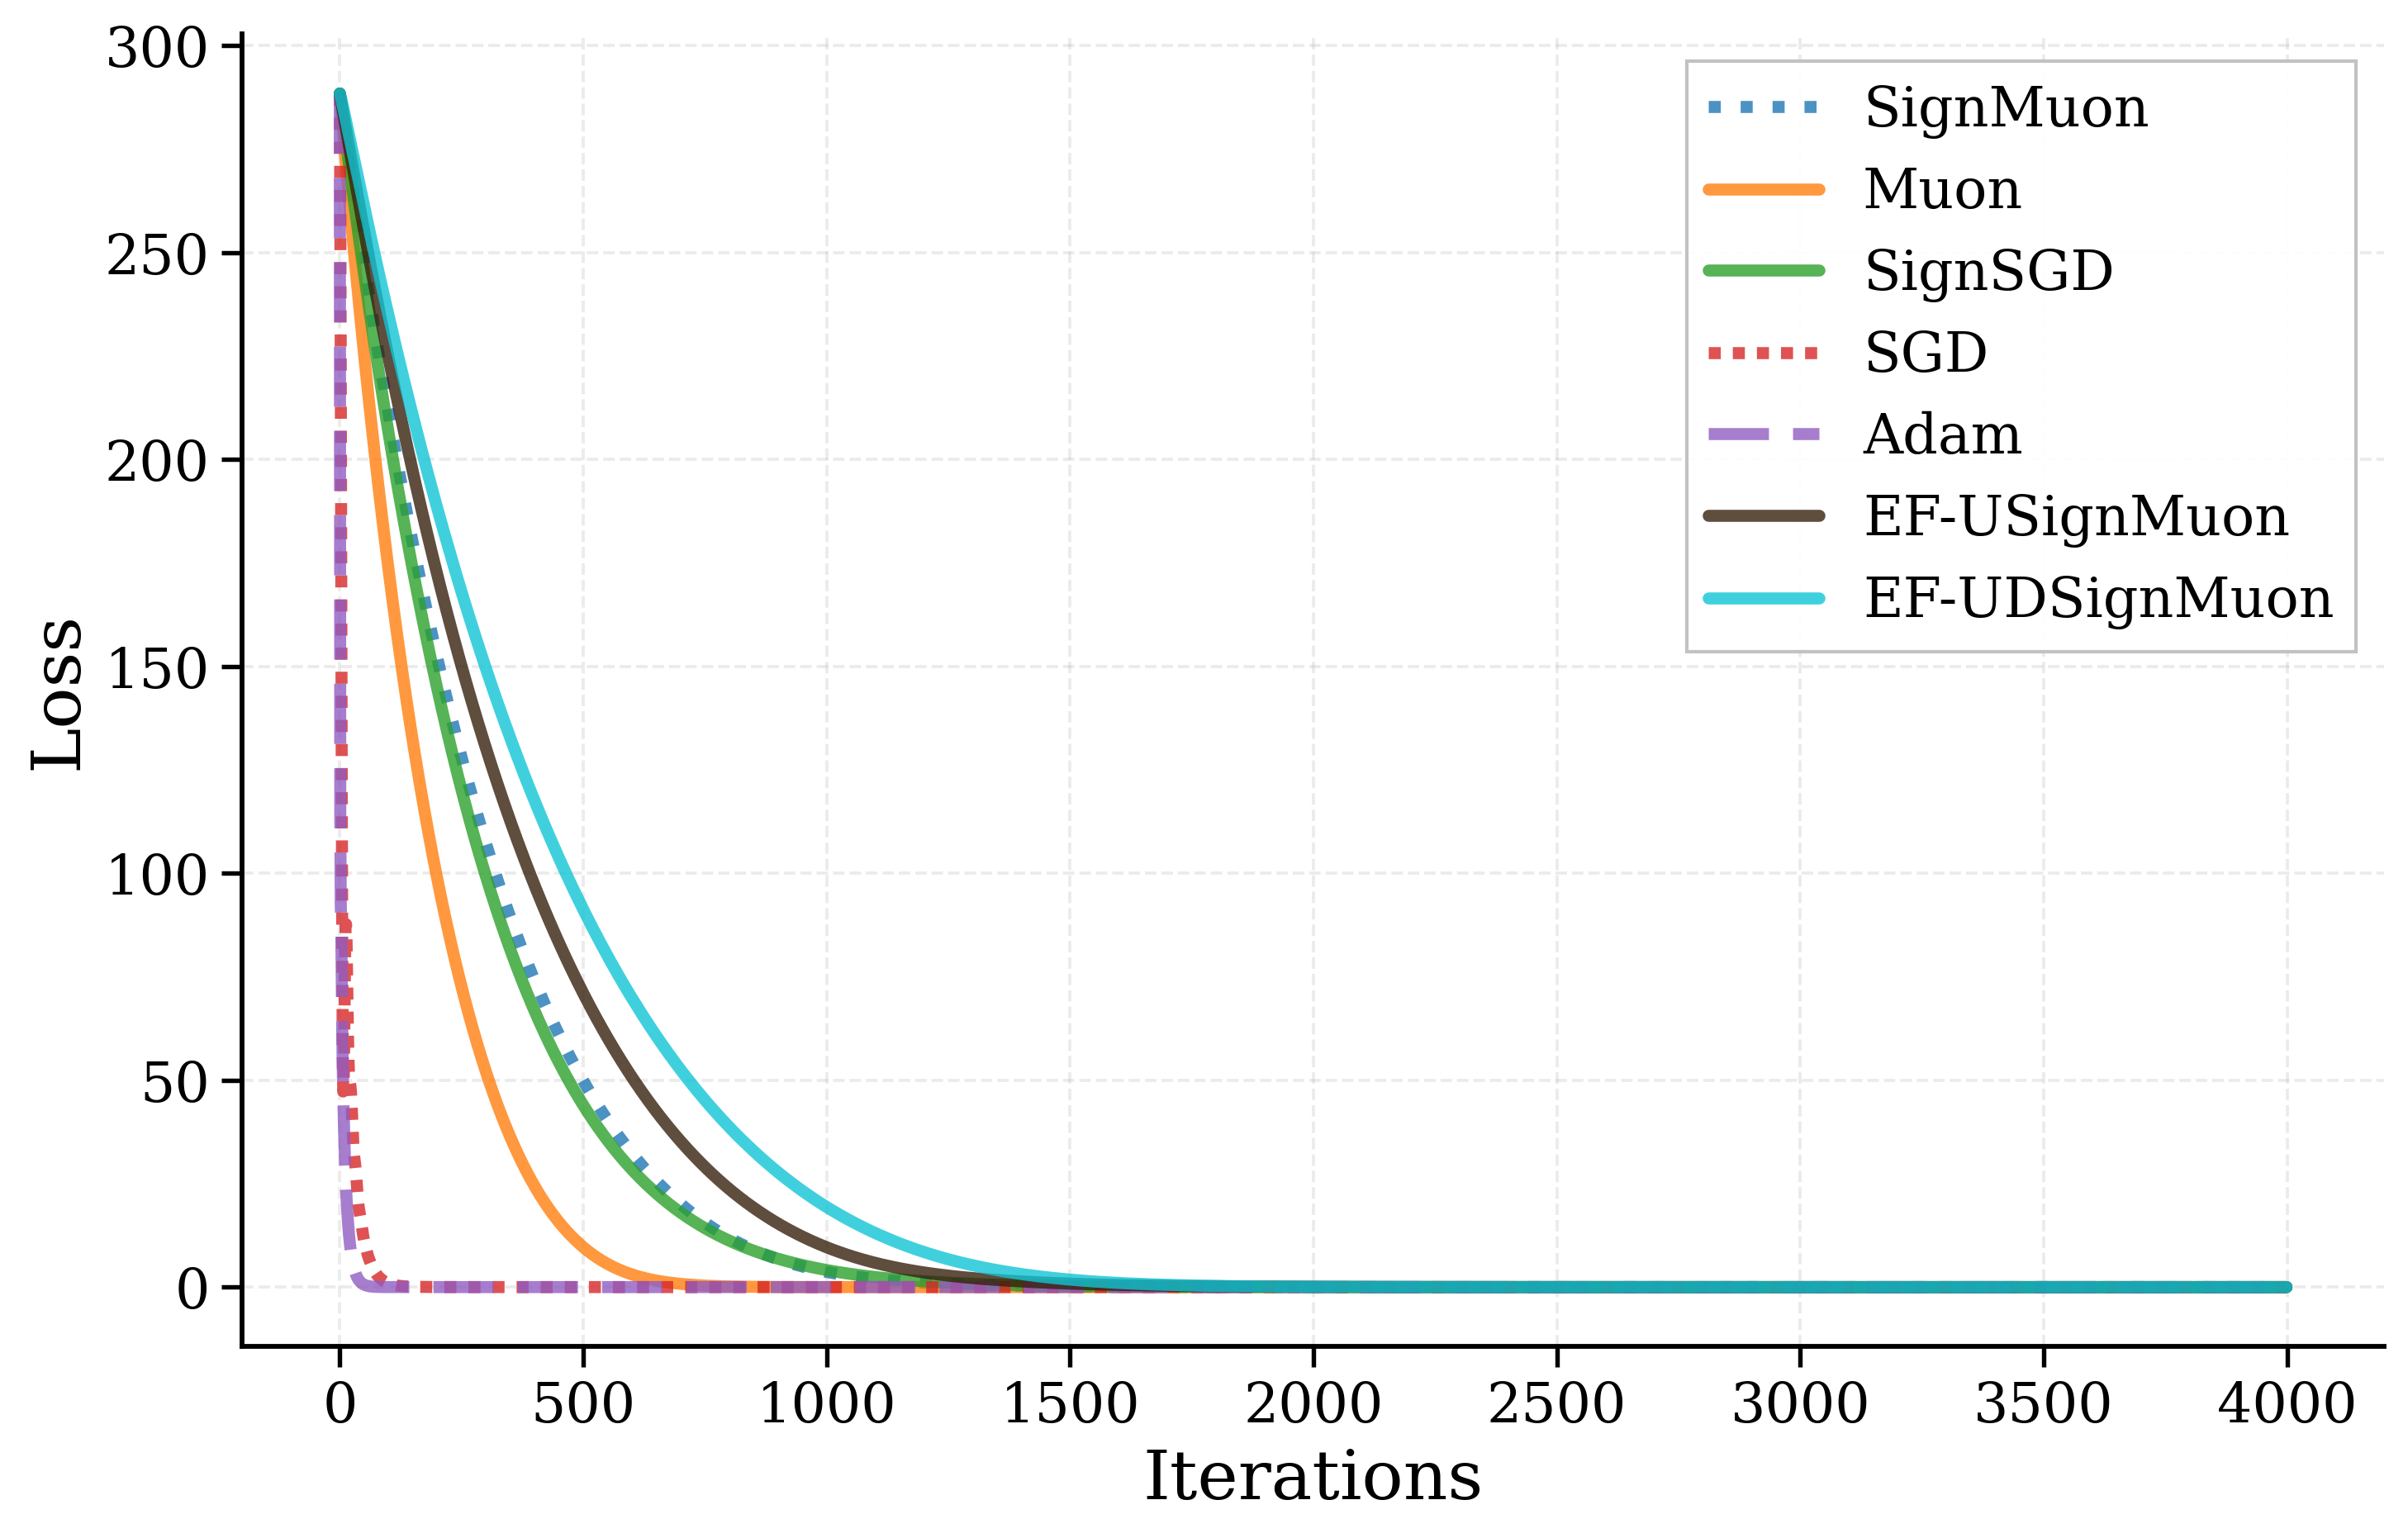
\includegraphics[width=\textwidth]{images/synt/loss.png} 
        \caption{Loss}
        \label{fig:synthetic_results_loss}
    \end{subfigure}
    \hfill
    \begin{subfigure}[b]{0.48\textwidth}
        \centering
        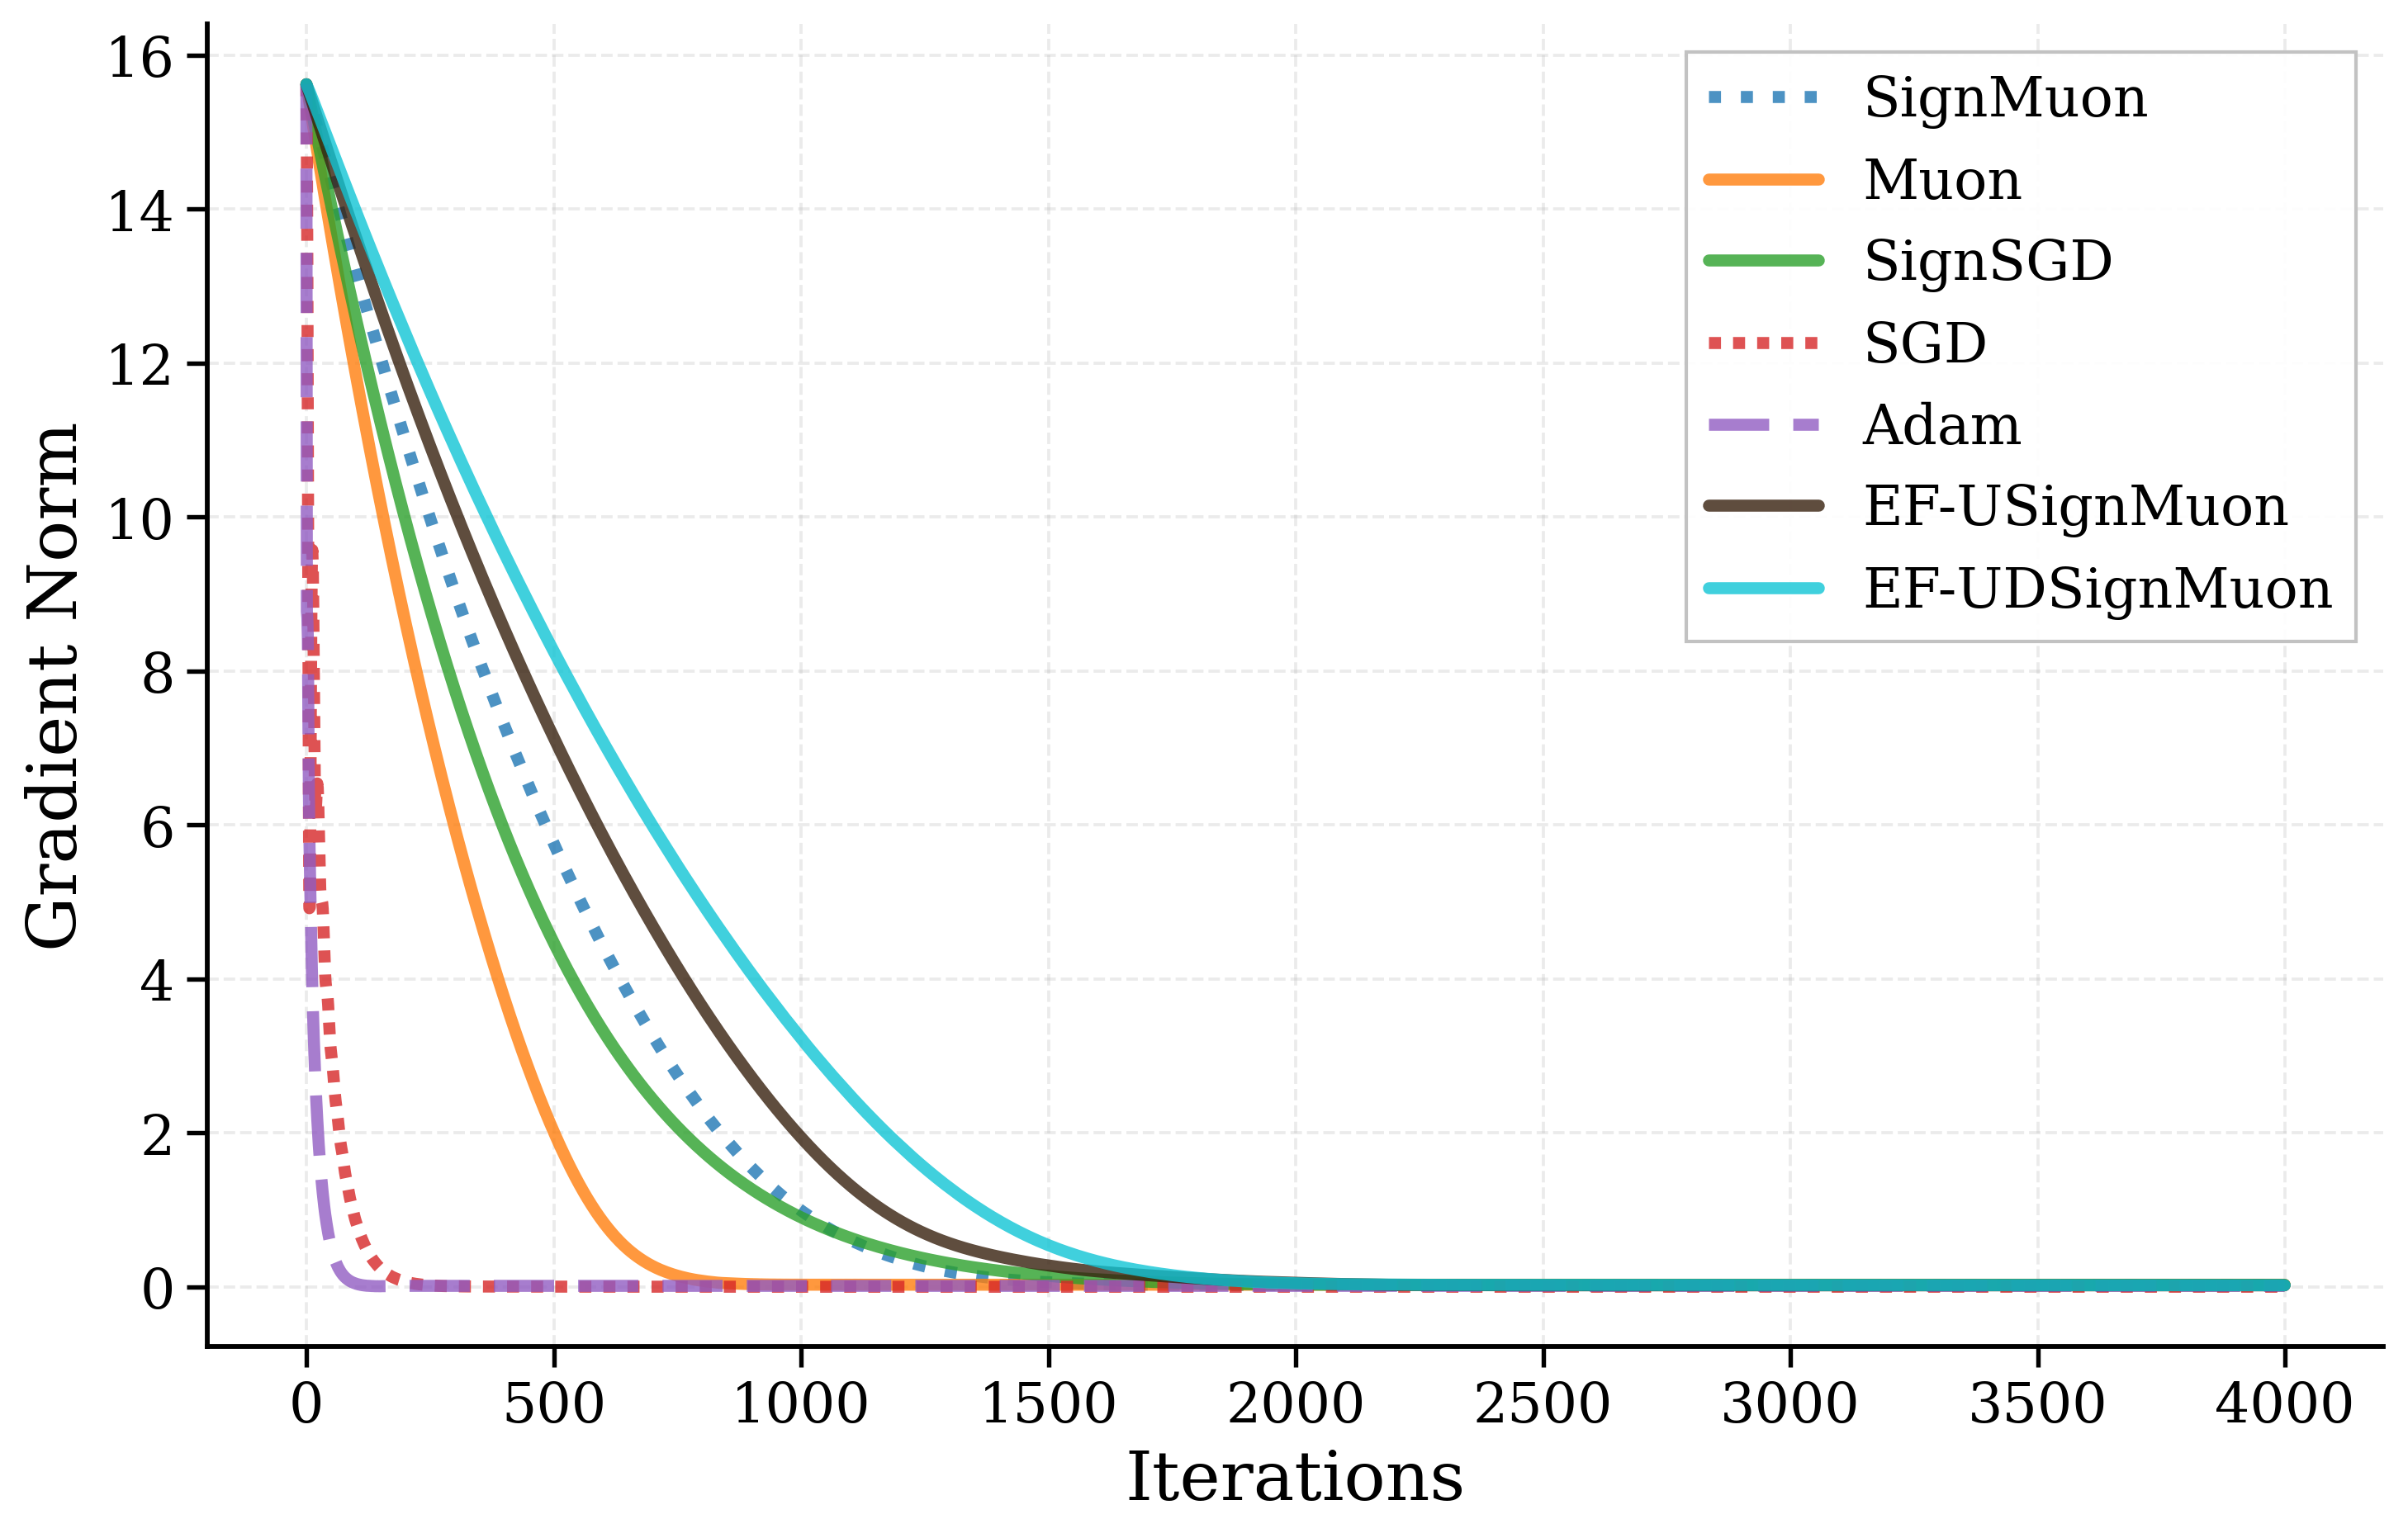
\includegraphics[width=\textwidth]{images/synt/GN.png} 
        \caption{Frobenius norm of the gradient}
        \label{fig:synthetic_results_GN}
    \end{subfigure}
    \caption{Smooth convex problem (Equation~\ref{eq:synthetic_problem} for $500\times500$).}
    \label{fig:synthetic_results}
\end{figure*}

\subsection{Centralized training results}\label{app:images_cen}
Table~\ref{tab:cifar_central} reports the centralized CIFAR-10 results on ResNet-18, including the tuned hyperparameters and the final train/test accuracies.
\begin{table*}[!t]
\centering
\small
\renewcommand{\arraystretch}{1.2}
\begin{tabular}{|c|c|c|c|c|c|c|c|c|c|}
\hline
\textbf{Dataset} & \textbf{Optimizer} & \textbf{Epoch} & \textbf{Batch} & \textbf{LR} & \textbf{LR Aux} & \textbf{Mom} & \textbf{Train Acc} & \textbf{Test Acc} \\
\hline
\multirow{6}{*}{CIFAR-10} & SignMuon & \multirow{6}{*}{75} & \multirow{6}{*}{128} & 0.001 & 0.0001 & \multirow{6}{*}{0.9} & 99.69\% & 92.55\% \\
\cline{2-2} \cline{5-6} \cline{8-9}
 & Muon & & & \multirow{2}{*}{0.015}  & \multirow{2}{*}{0.001} & & 99.94\% & 93.70\% \\
 \cline{2-2} \cline{8-9}
& SGD & & & & & & 99.98\% & 93.93\% \\
\cline{2-2} \cline{5-6} \cline{8-9}
& SignSGD & & & \multirow{2}{*}{0.001}  & \multirow{2}{*}{0.0001}  & & 93.19\% & 89.11\% \\
\cline{2-2} \cline{8-9}
 & Adam & & &  & & & 99.77\% & 93.03\% \\
 \cline{2-2} \cline{5-6} \cline{8-9}
 & EF21-MuonUSign & & & 0.008 & 0.001& & 99.96\% & 93.82\% \\
\hline
\end{tabular}
\caption{CIFAR-10: Centralized Learning on ResNet-18.}
\label{tab:cifar_central}
\end{table*}

% \begin{figure*}[!t]
%     \centering
%     \begin{subfigure}[b]{0.48\textwidth}
%         \centering
%         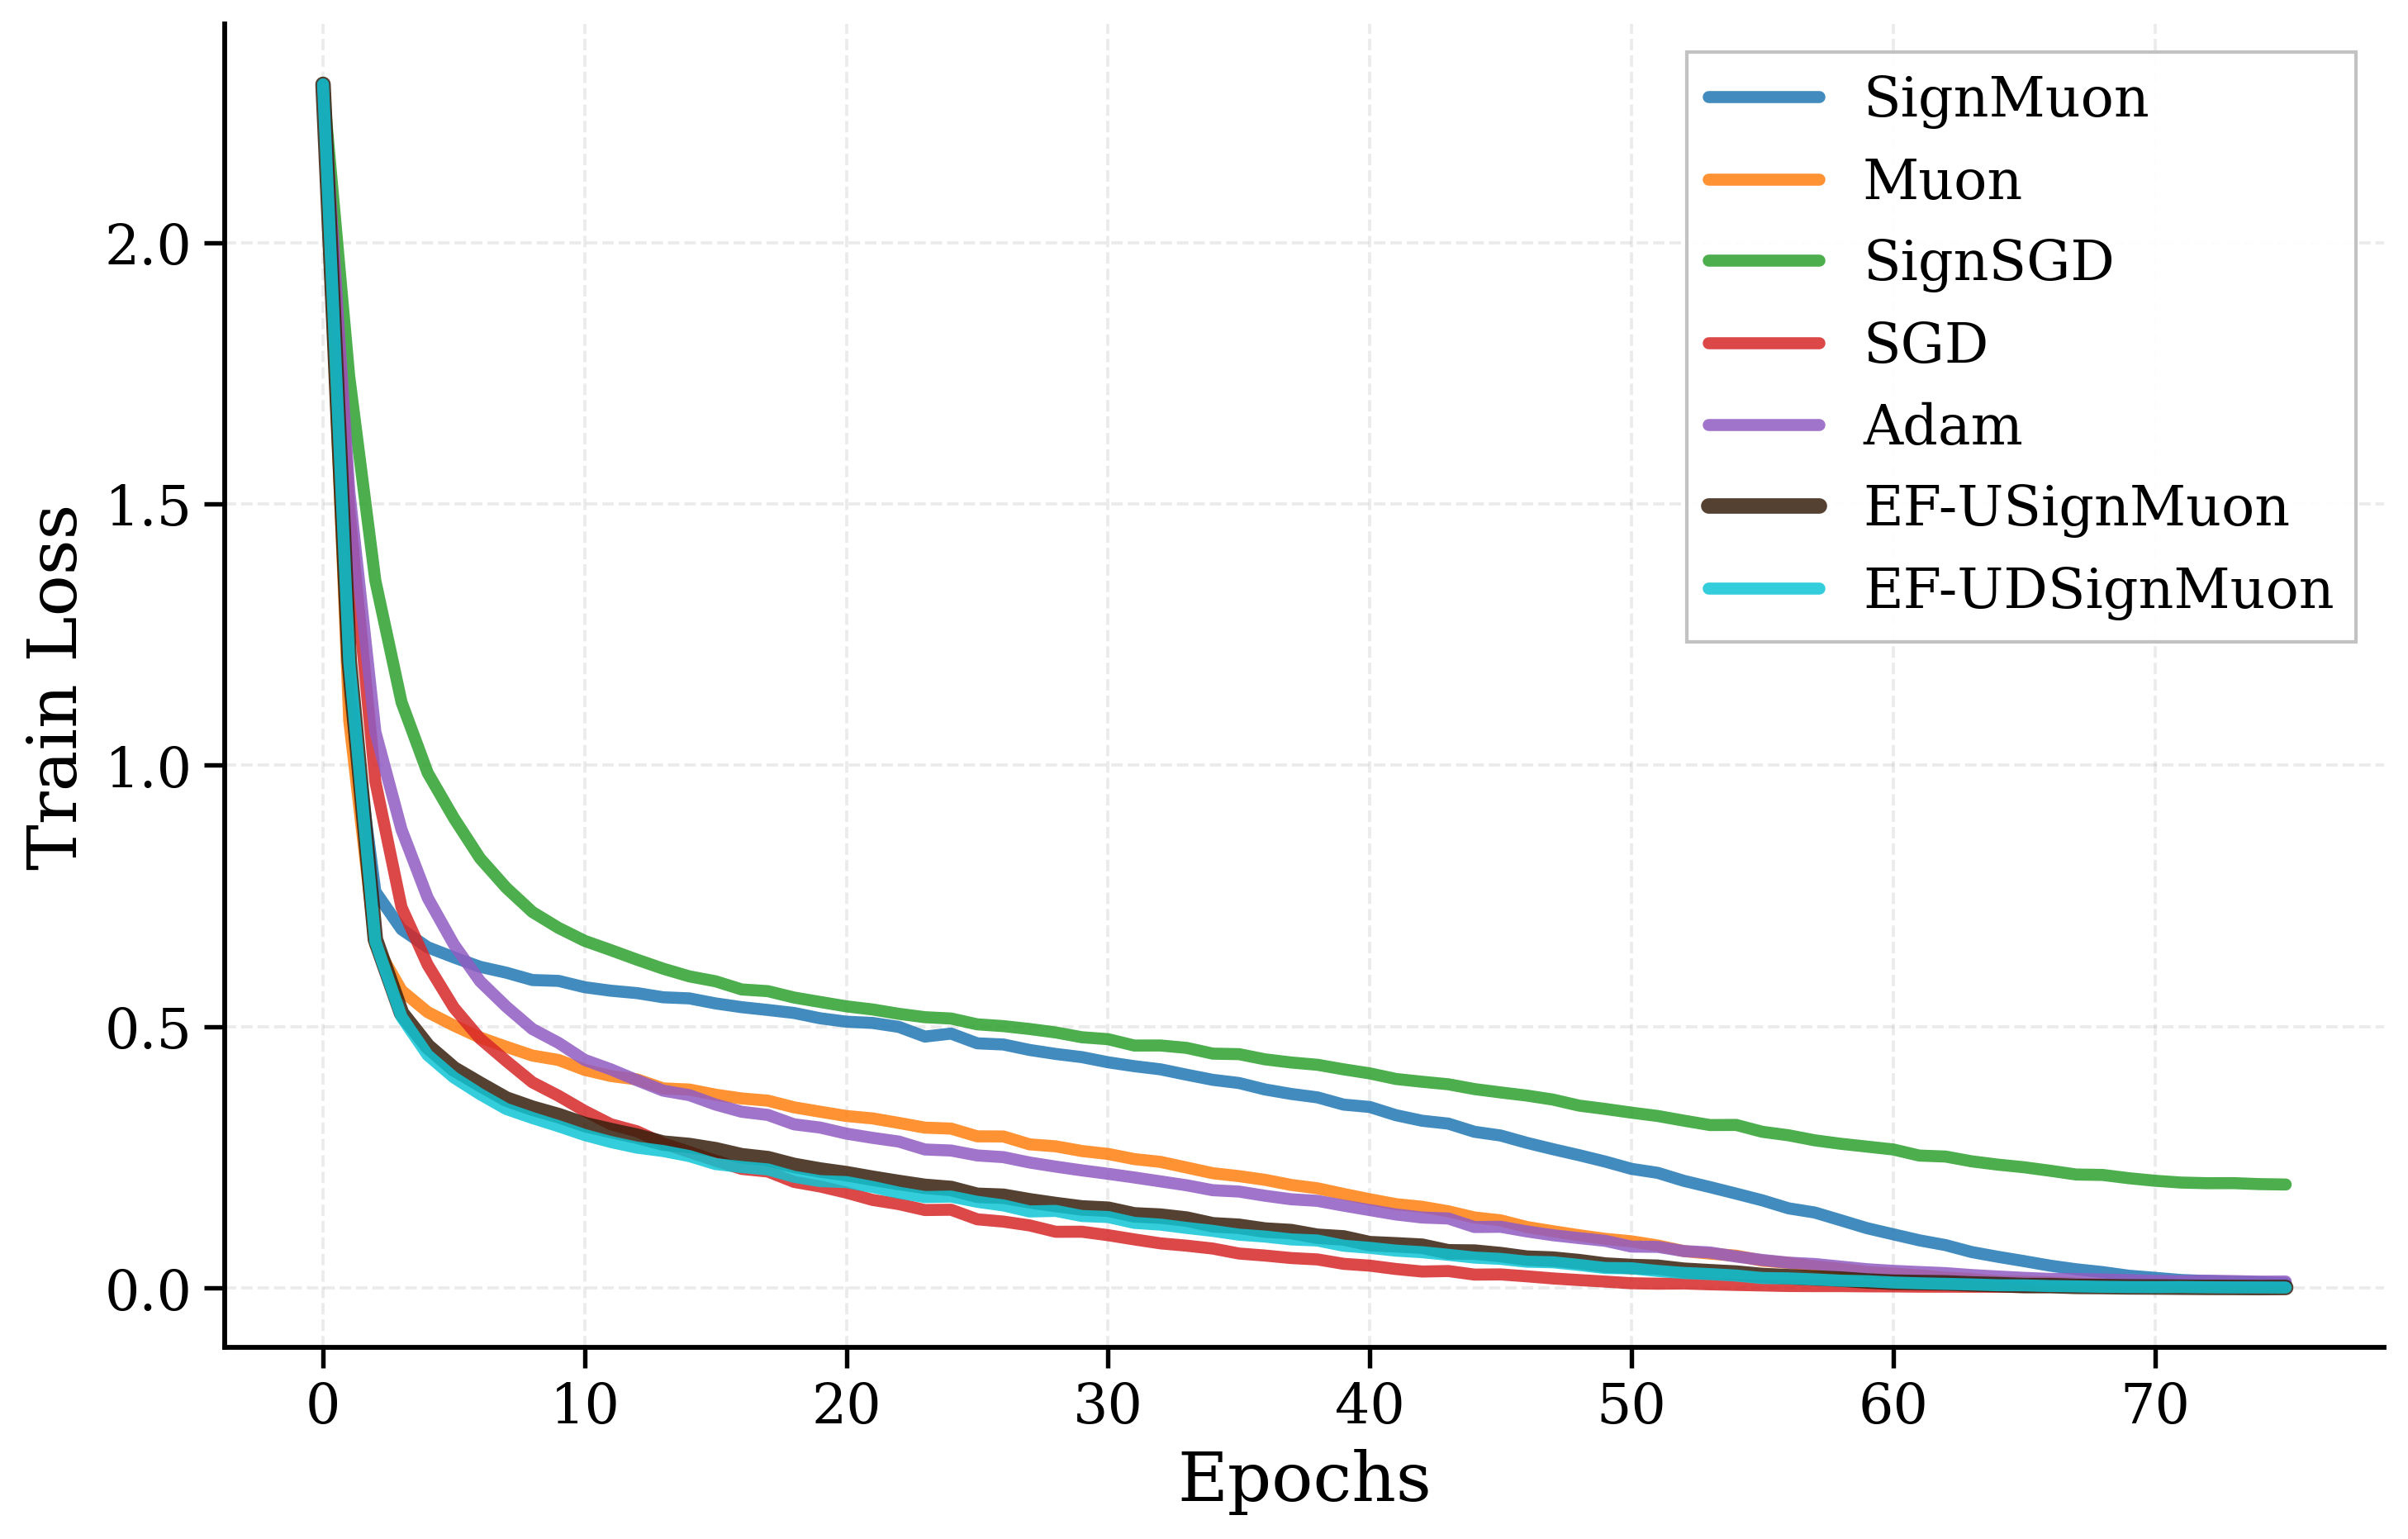
\includegraphics[width=\textwidth]{images/centralized_images/train_loss_resnet.png} 
%         \caption{Train Loss}
%     \end{subfigure}
%     \hfill
%     \begin{subfigure}[b]{0.48\textwidth}
%         \centering
%         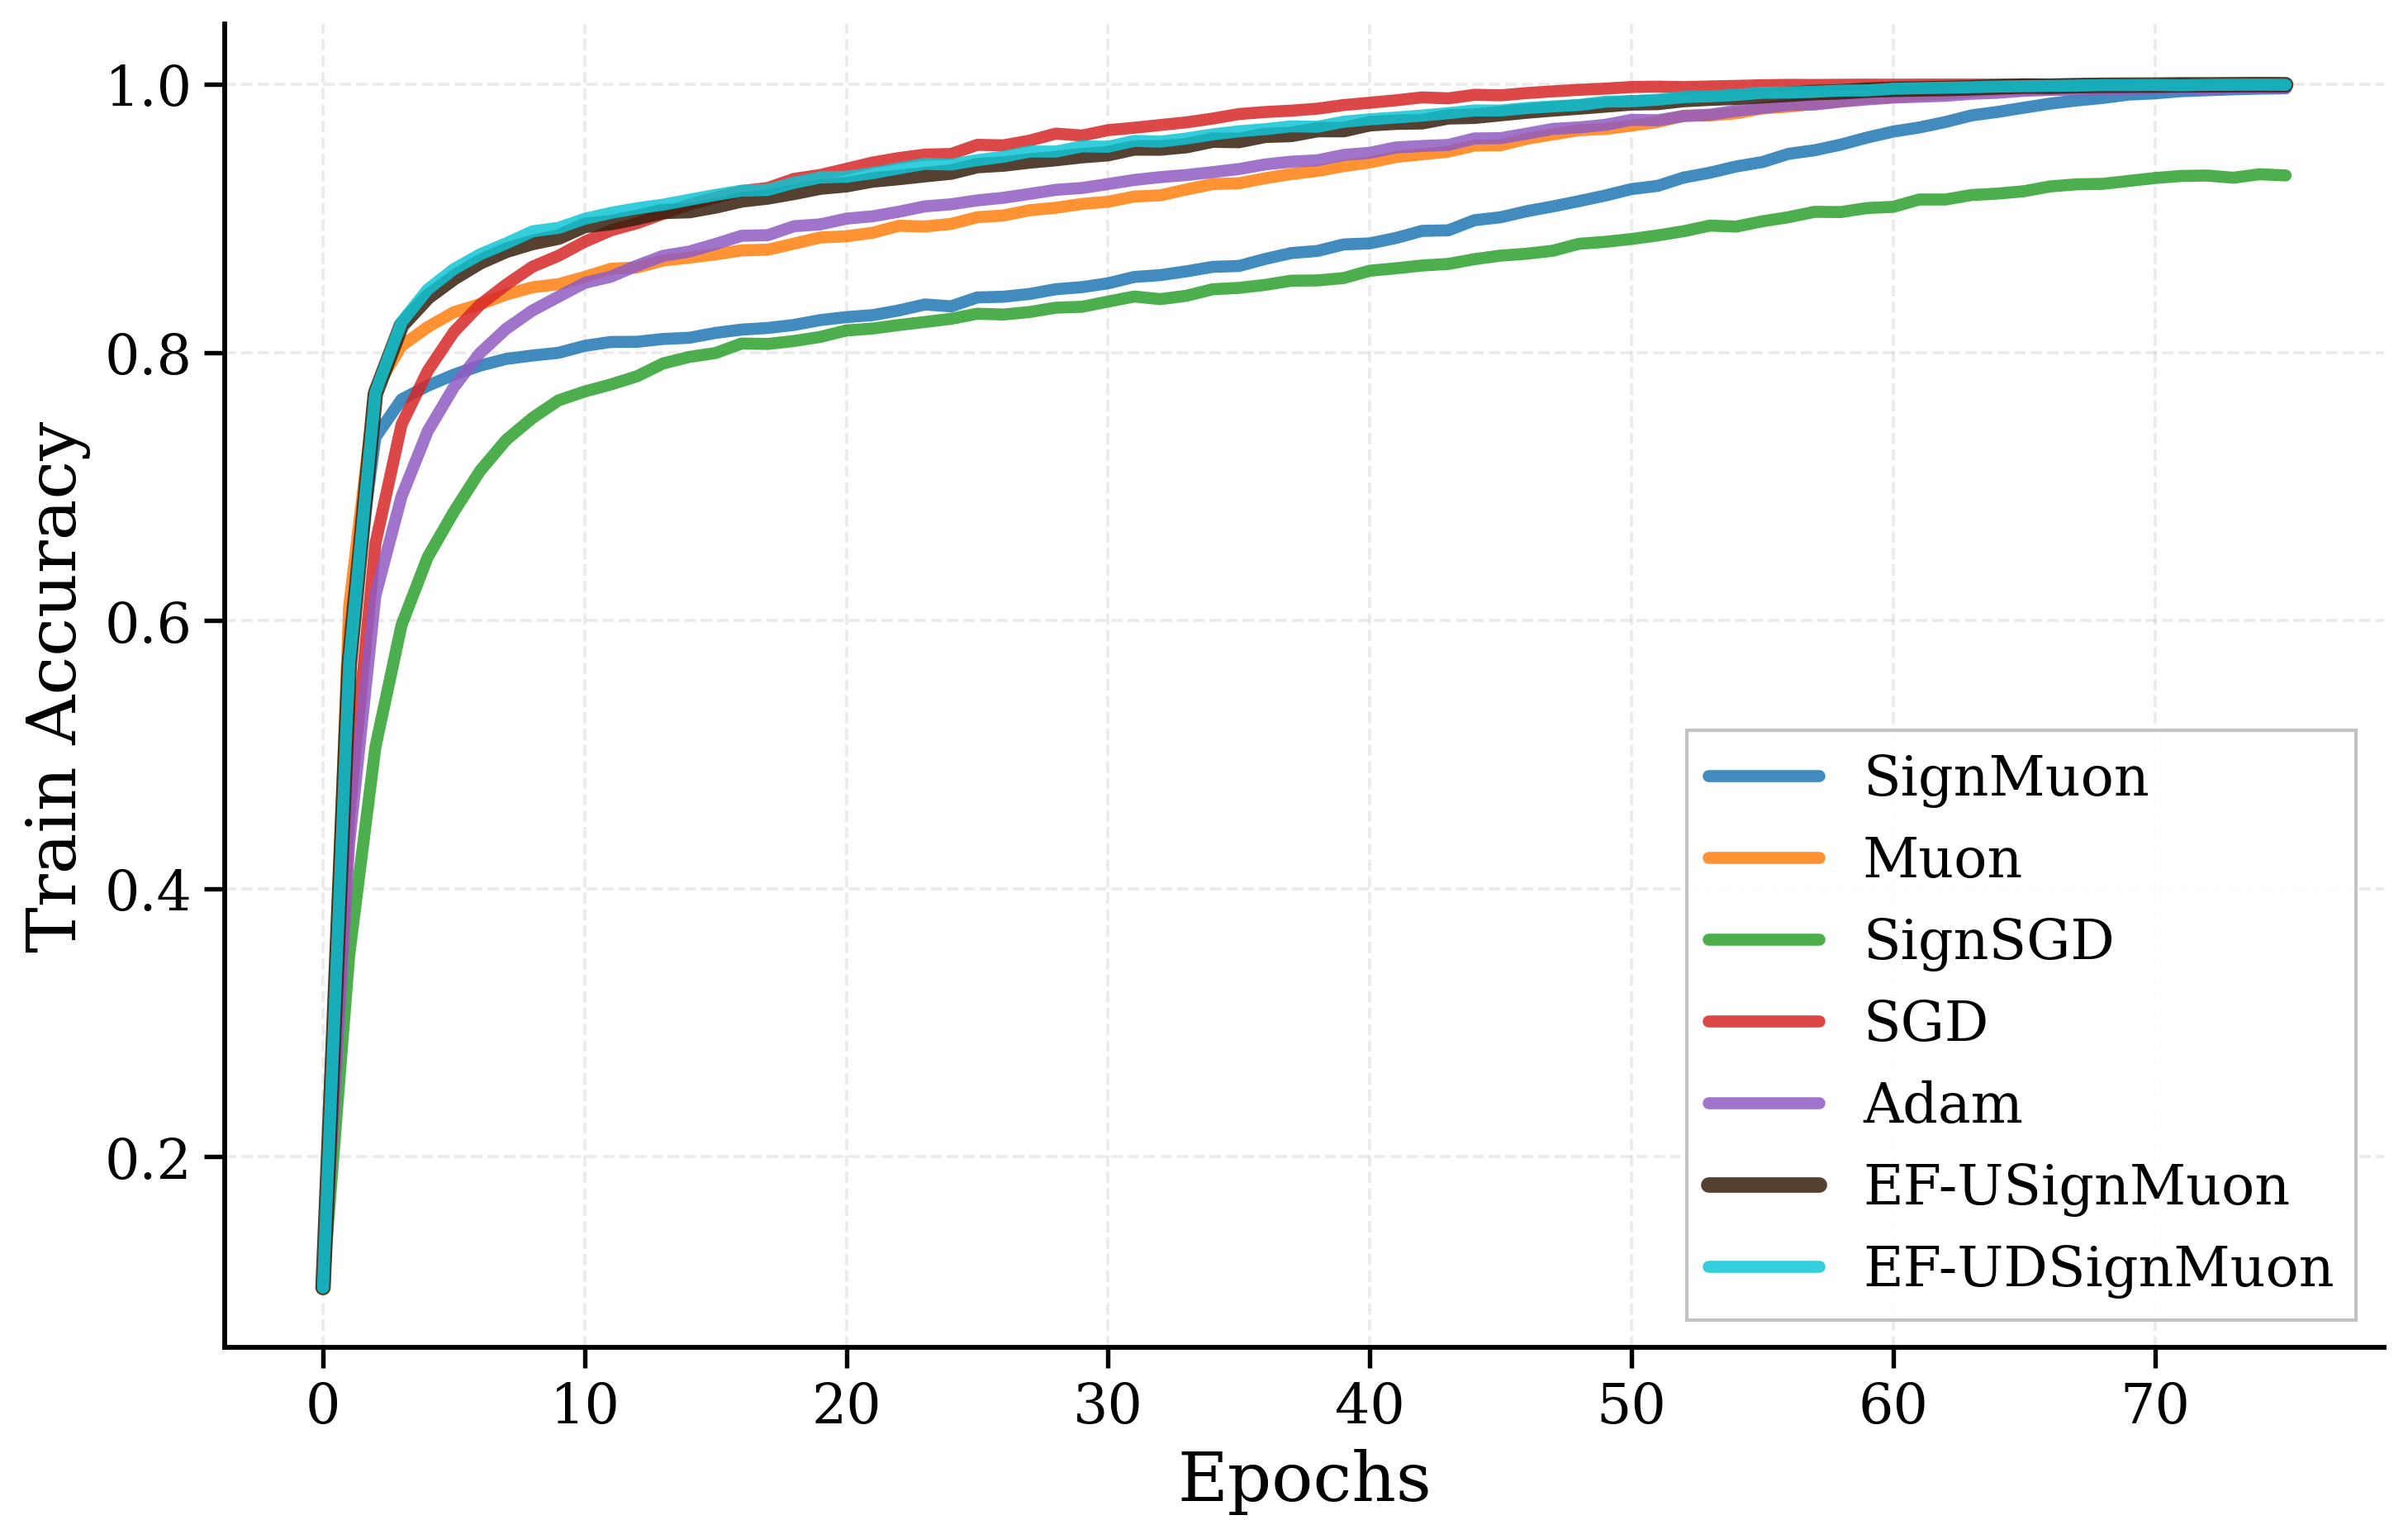
\includegraphics[width=\textwidth]{images/centralized_images/train_acc_resnet.png} 
%         \caption{Train Accuracy}
%     \end{subfigure}
%     \caption{Centralized setting. Comparison of convergence and classification accuracy achieved by different optimization algorithms during CIFAR-10 classifier training on the training set on ResNet-18.}
%     \label{fig:cifar_results_train}
% \end{figure*}

% \newpage
\subsection{Federated training results. Experiment 1}\label{app:results_fed:1}
Table~\ref{tab:exp_1} and Figure~\ref{fig:exp_1} report the scalability of SignMuon with respect to the number of clients (Experiment~1).
\begin{table*}[!t]
\centering
\small
\renewcommand{\arraystretch}{1.2}
\begin{tabular}{|c|c|c|c|c|c|c|c|c|}
\hline
\textbf{Dataset} & \textbf{Optimizer} & \textbf{Rounds} & \textbf{Clients} & \textbf{Steps} & \textbf{Batch} & \textbf{LR} & \textbf{Mom} & \textbf{Test Acc} \\
\hline
\multirow{5}{*}{CIFAR-10} & \multirow{5}{*}{SignMuon} & \multirow{5}{*}{2000} & 1 & \multirow{5}{*}{1} & \multirow{5}{*}{64} & \multirow{5}{*}{0.001} & \multirow{5}{*}{0.9} & 76.13\% \\
\cline{4-4} \cline{9-9}
 & & & 3 & & & & & 81.24\% \\
\cline{4-4} \cline{9-9}
 & & & 5 & & & & & 82.87\% \\
\cline{4-4} \cline{4-4} \cline{9-9}
 & & & 7 & & & & & 83.54\% \\
\cline{4-4} \cline{9-9}
 & & & 9 & & & & & 84.03\% \\
\hline
\end{tabular}
\caption{CIFAR-10 Federated Learning on CNN2. Experiment 1. Scalability of the SignMuon Algorithm.}
\label{tab:exp_1}
\end{table*}

\begin{figure*}[!t]
    \centering
    \begin{subfigure}[b]{0.48\textwidth}
        \centering
        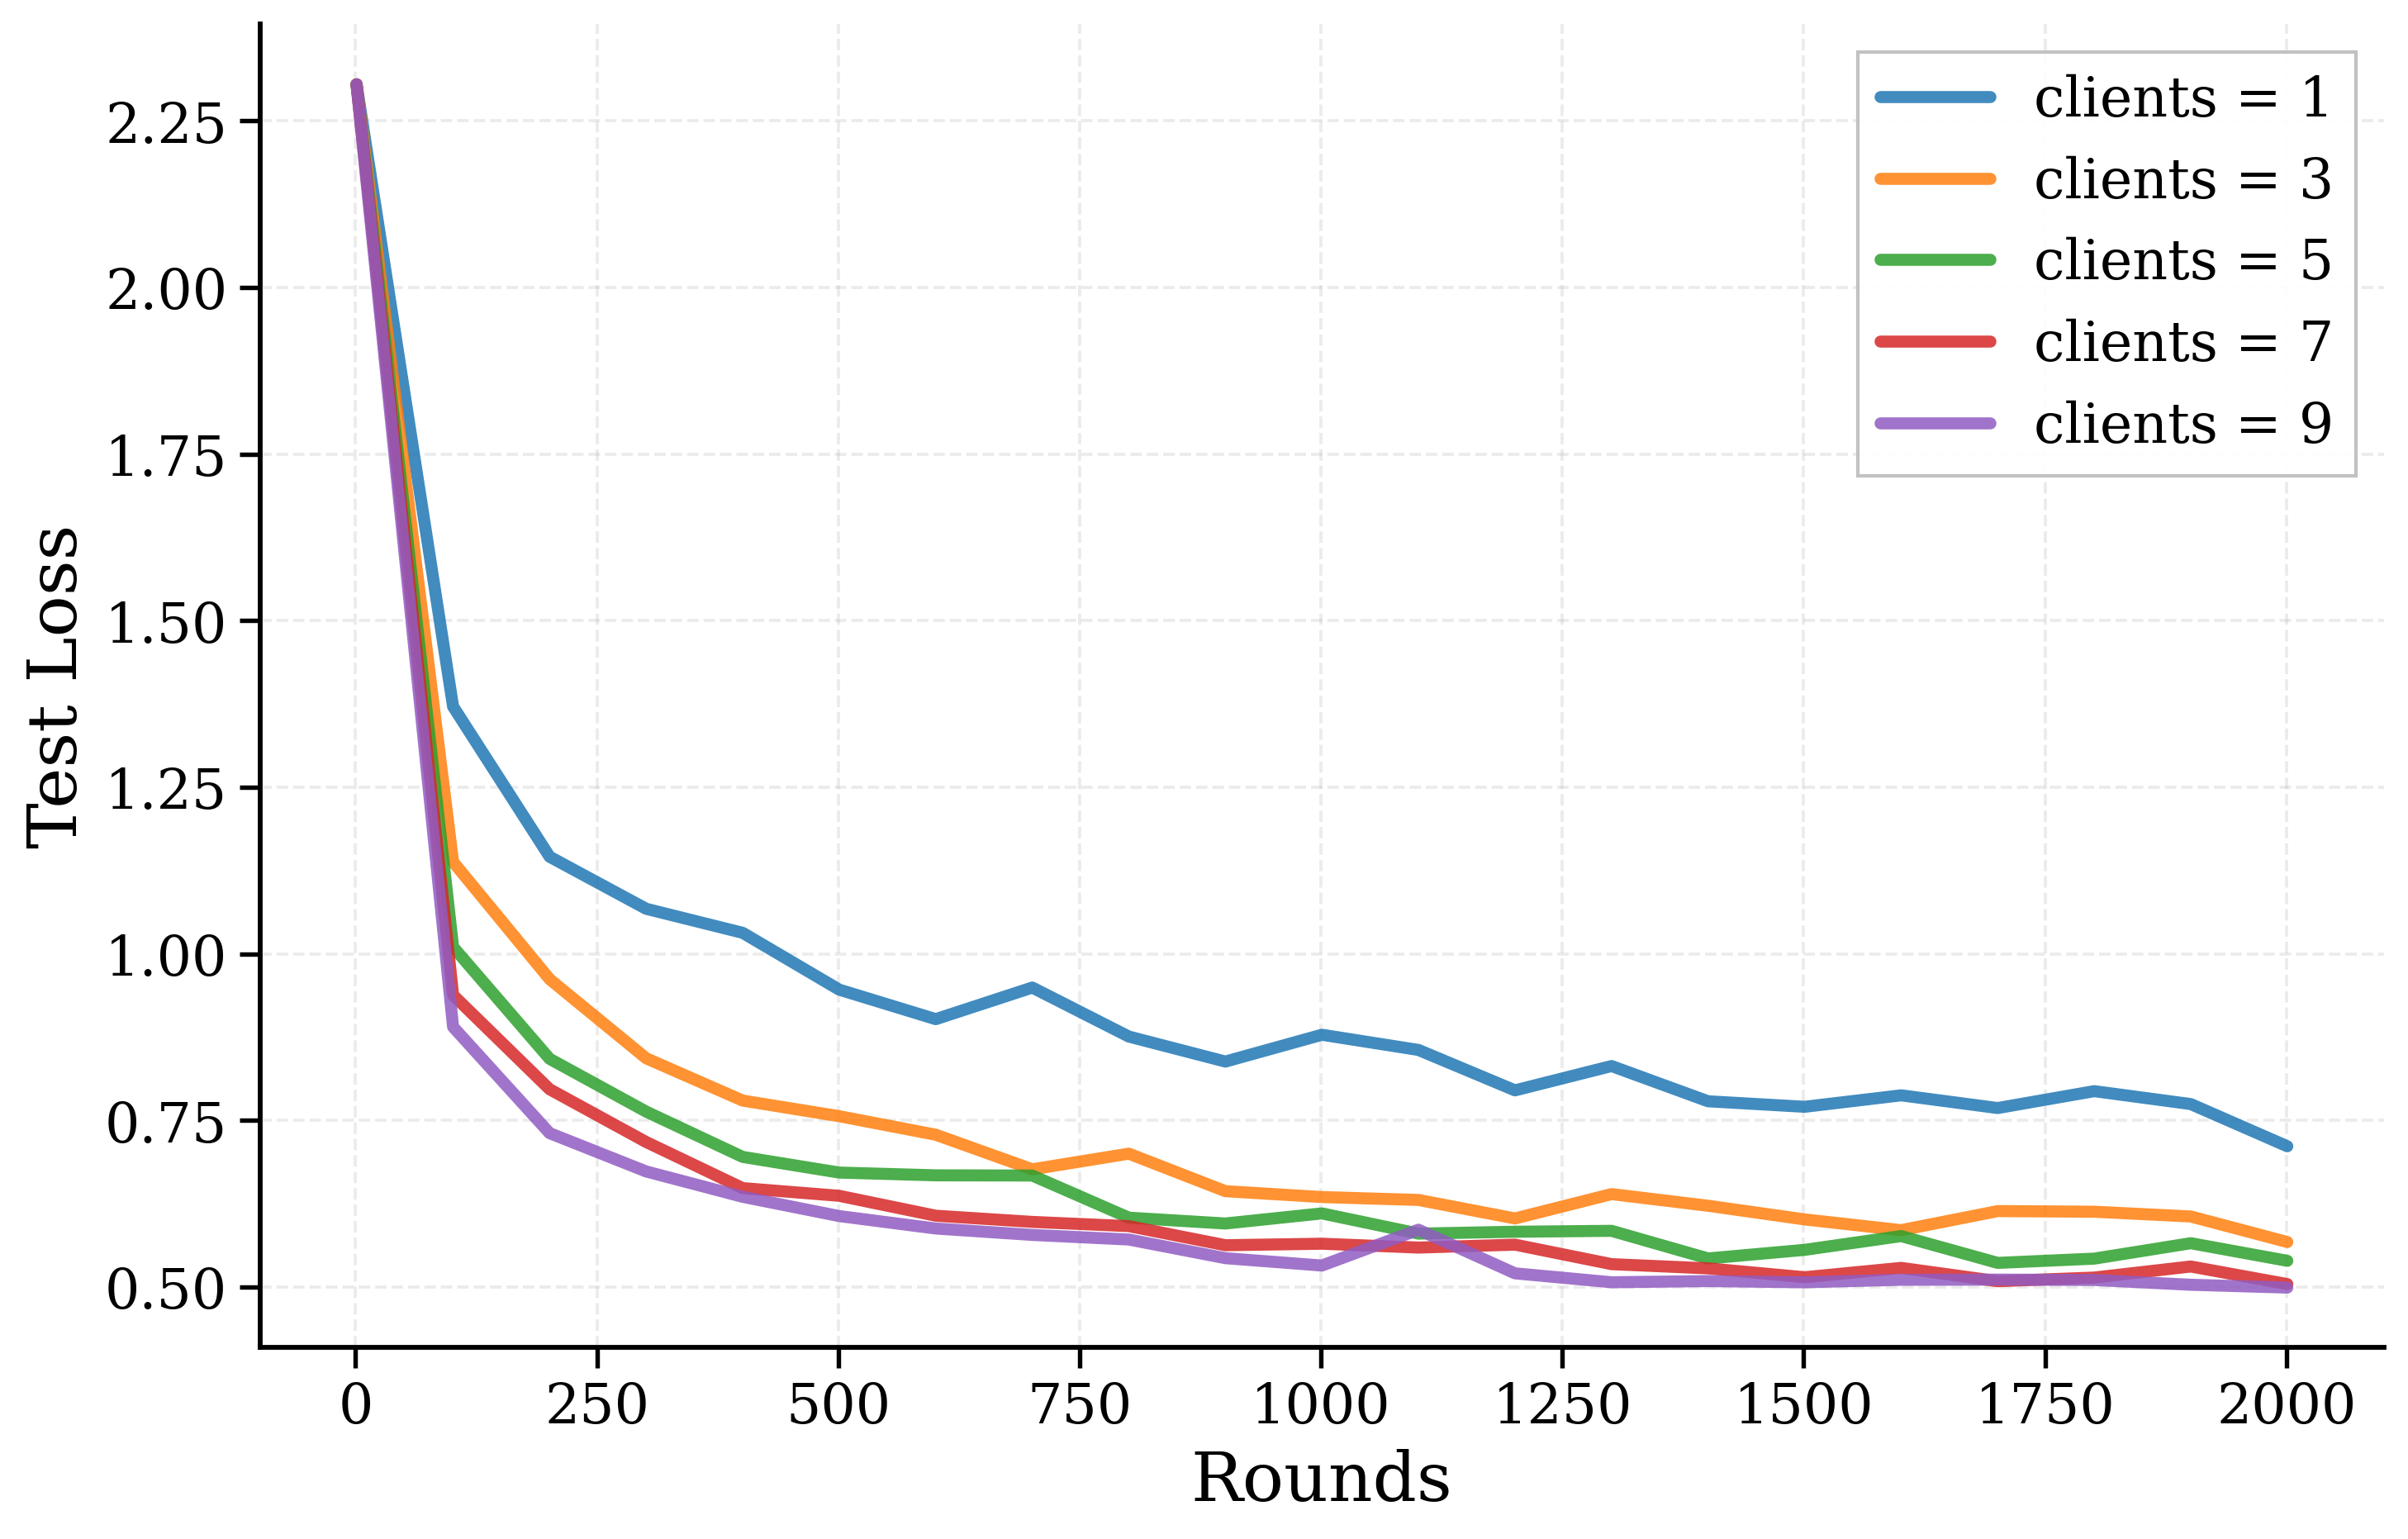
\includegraphics[width=\textwidth]{images/federated_images/signmuon_loss.png} 
        \caption{Test Loss}
    \end{subfigure}
    \hfill
    \begin{subfigure}[b]{0.48\textwidth}
        \centering
        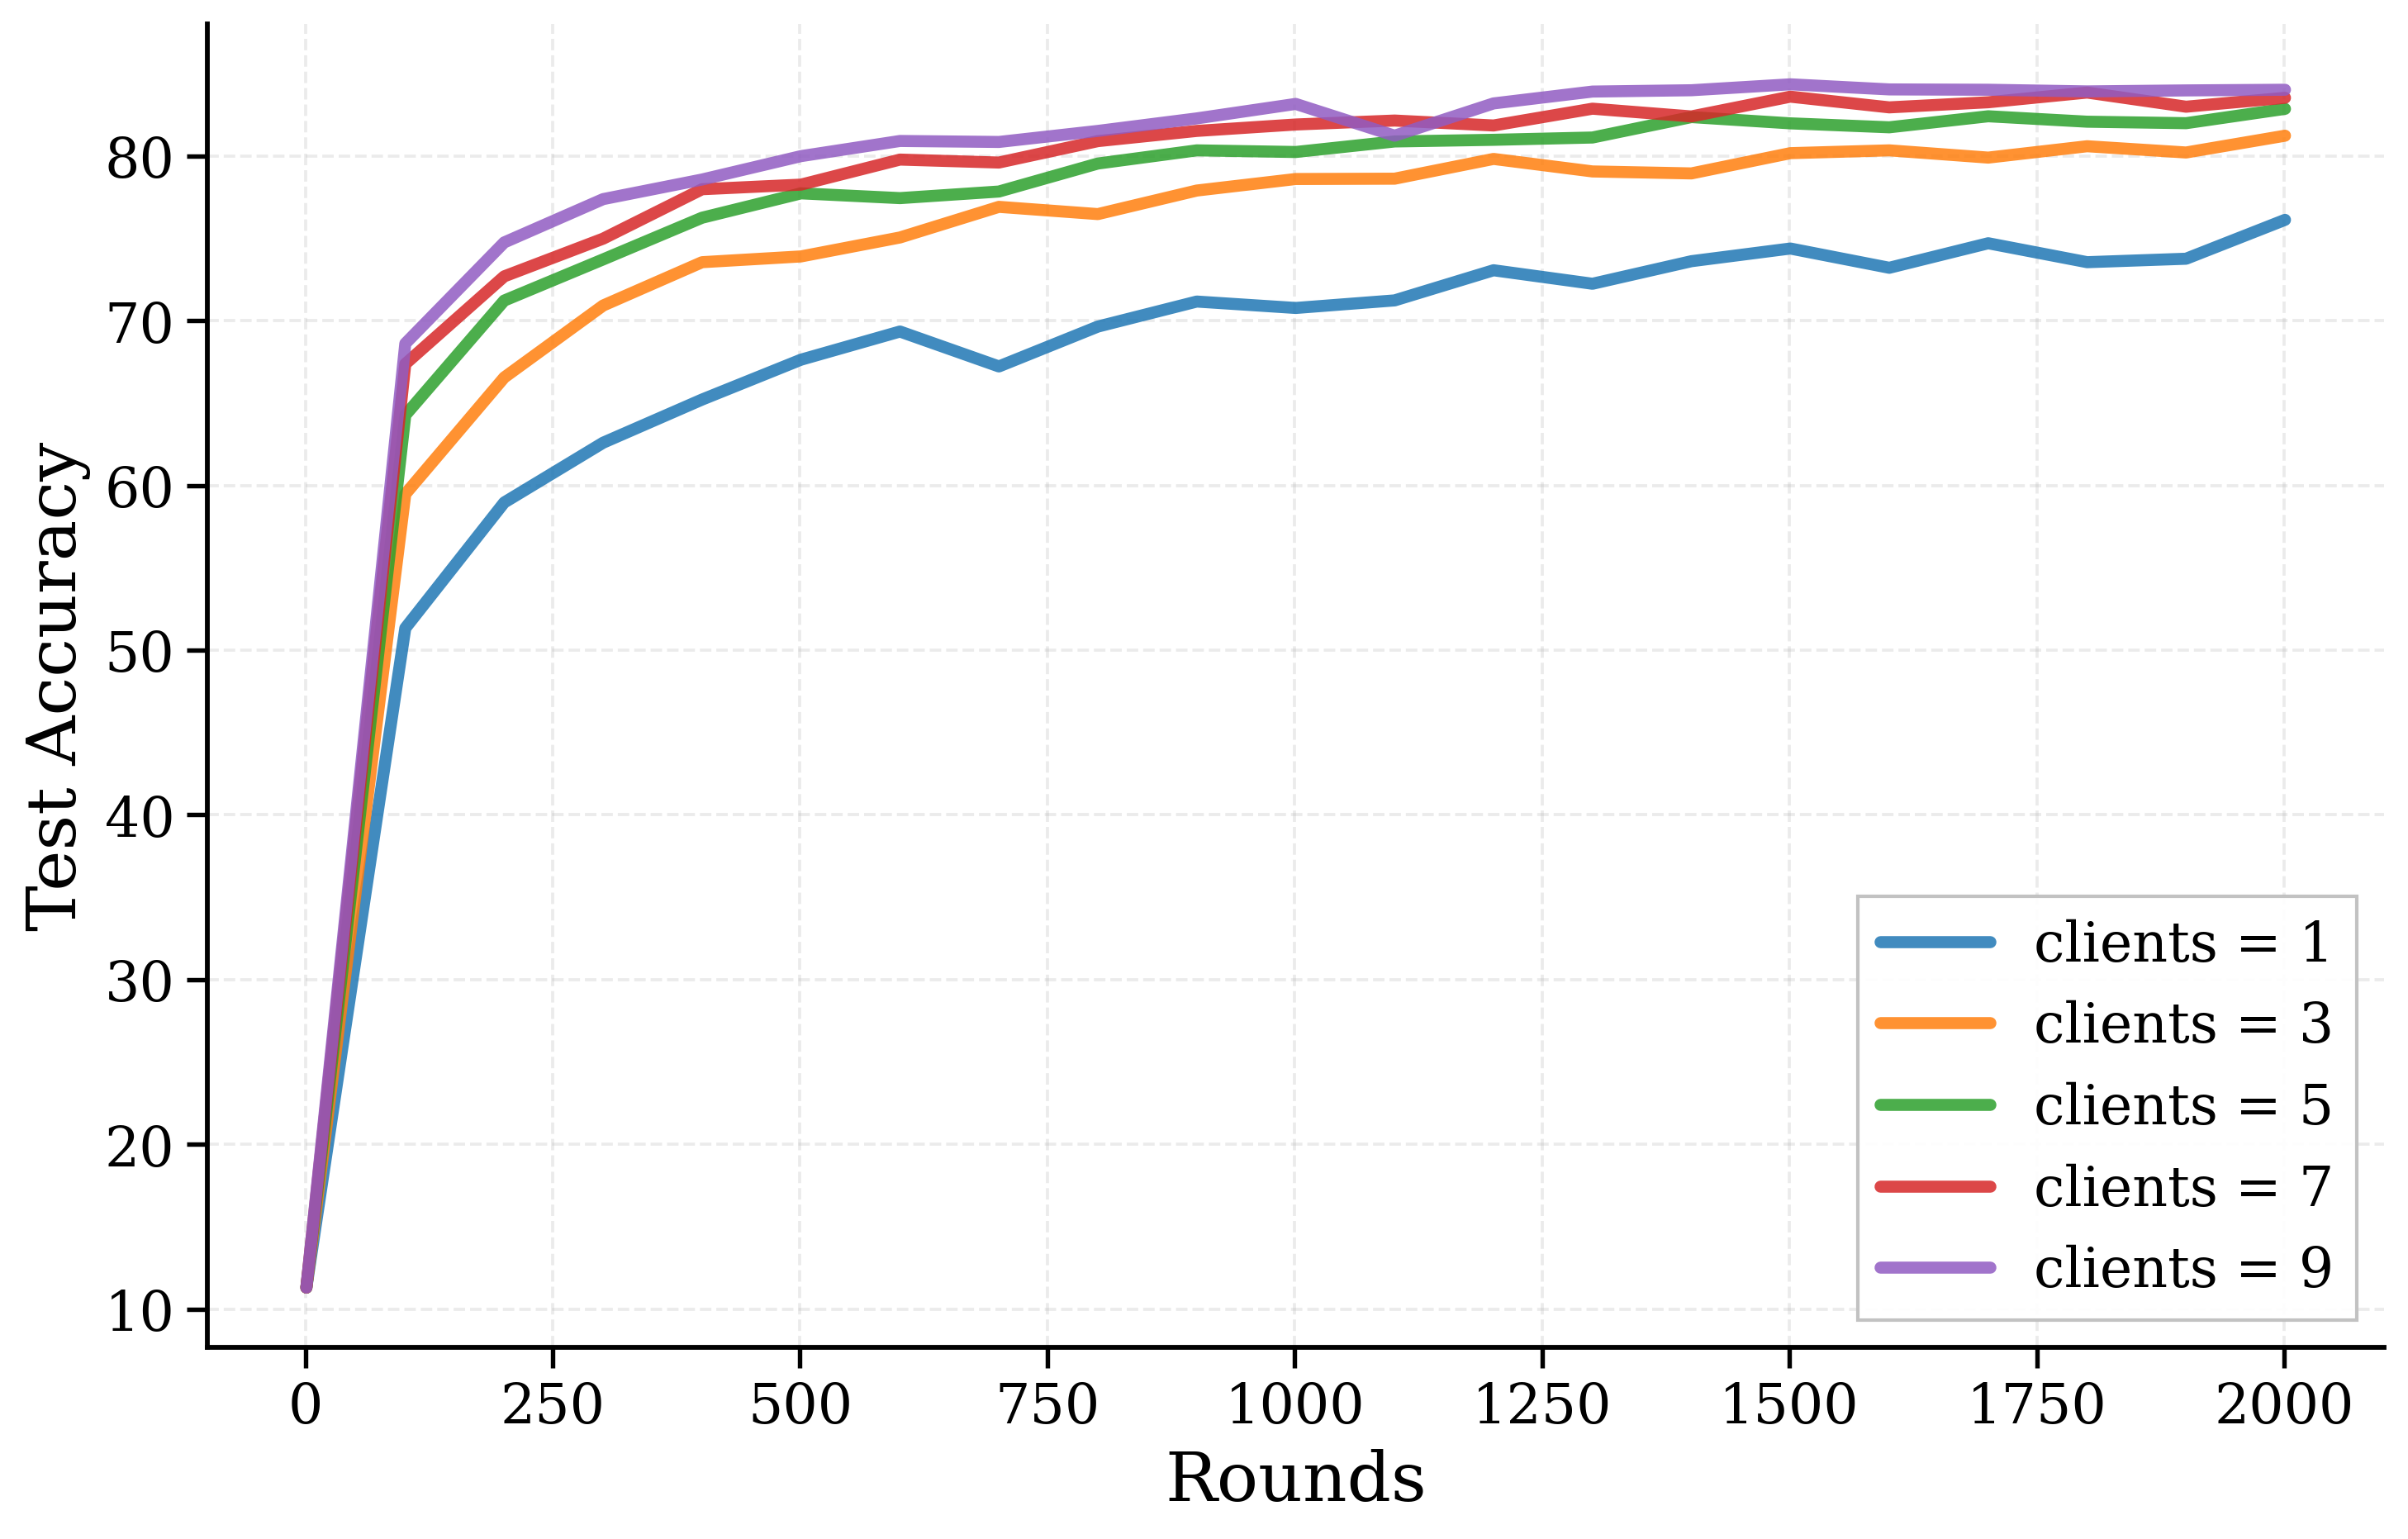
\includegraphics[width=\textwidth]{images/federated_images/signmuon_acc.png}
        \caption{Test Accuracy}
    \end{subfigure}
    \caption{CIFAR-10 Federated Learning on CNN2. Experiment 1. Scalability of the SignMuon Algorithm.}
    \label{fig:exp_1}
\end{figure*}


\subsection{Federated training results. Experiment 2}\label{app:results_fed:2}
Table~\ref{tab:exp_2} and Figure~\ref{fig:exp_2} report the comparison of optimizers with $N=3$ clients (Experiment~2).
\begin{table*}[!t]
\centering
\small
\renewcommand{\arraystretch}{1.2}
\begin{tabular}{|c|c|c|c|c|c|c|c|c|}
\hline
\textbf{Dataset} & \textbf{Optimizer} & \textbf{Rounds} & \textbf{Clients} & \textbf{Steps} & \textbf{Batch} & \textbf{LR} & \textbf{Mom} & \textbf{Test Acc} \\
\hline
\multirow{6}{*}{CIFAR-10} & SignMuon & \multirow{6}{*}{2000} & \multirow{6}{*}{3} & \multirow{6}{*}{1} & \multirow{6}{*}{64} & 0.001 & \multirow{6}{*}{0.9} & 81.24\% \\
\cline{2-2} \cline{7-7} \cline{9-9}
 & Muon & & & & & 0.05 & & 81.27\% \\
\cline{2-2} \cline{7-7} \cline{9-9}
 & SignSGD & & & & & 0.001 & & 65.96\% \\
\cline{2-2} \cline{7-7} \cline{9-9}
 & SGD & & & & & 0.03 & & 76.77\% \\
\cline{2-2} \cline{7-7} \cline{9-9}
 & Adam & & & & & 0.001 & & 70.83\% \\
\cline{2-2} \cline{7-7} \cline{9-9}
 & EF21-MuonUSign & & & & & 0.02 & & 80.69\% \\
\hline
\end{tabular}
\caption{CIFAR-10 Federated Learning on CNN2. Experiment 2: Comparison of Optimization Algorithms with (N = 3) Clients.}
\label{tab:exp_2}
\end{table*}

\begin{figure*}[!t]
    \centering
    \begin{subfigure}[b]{0.48\textwidth}
        \centering
        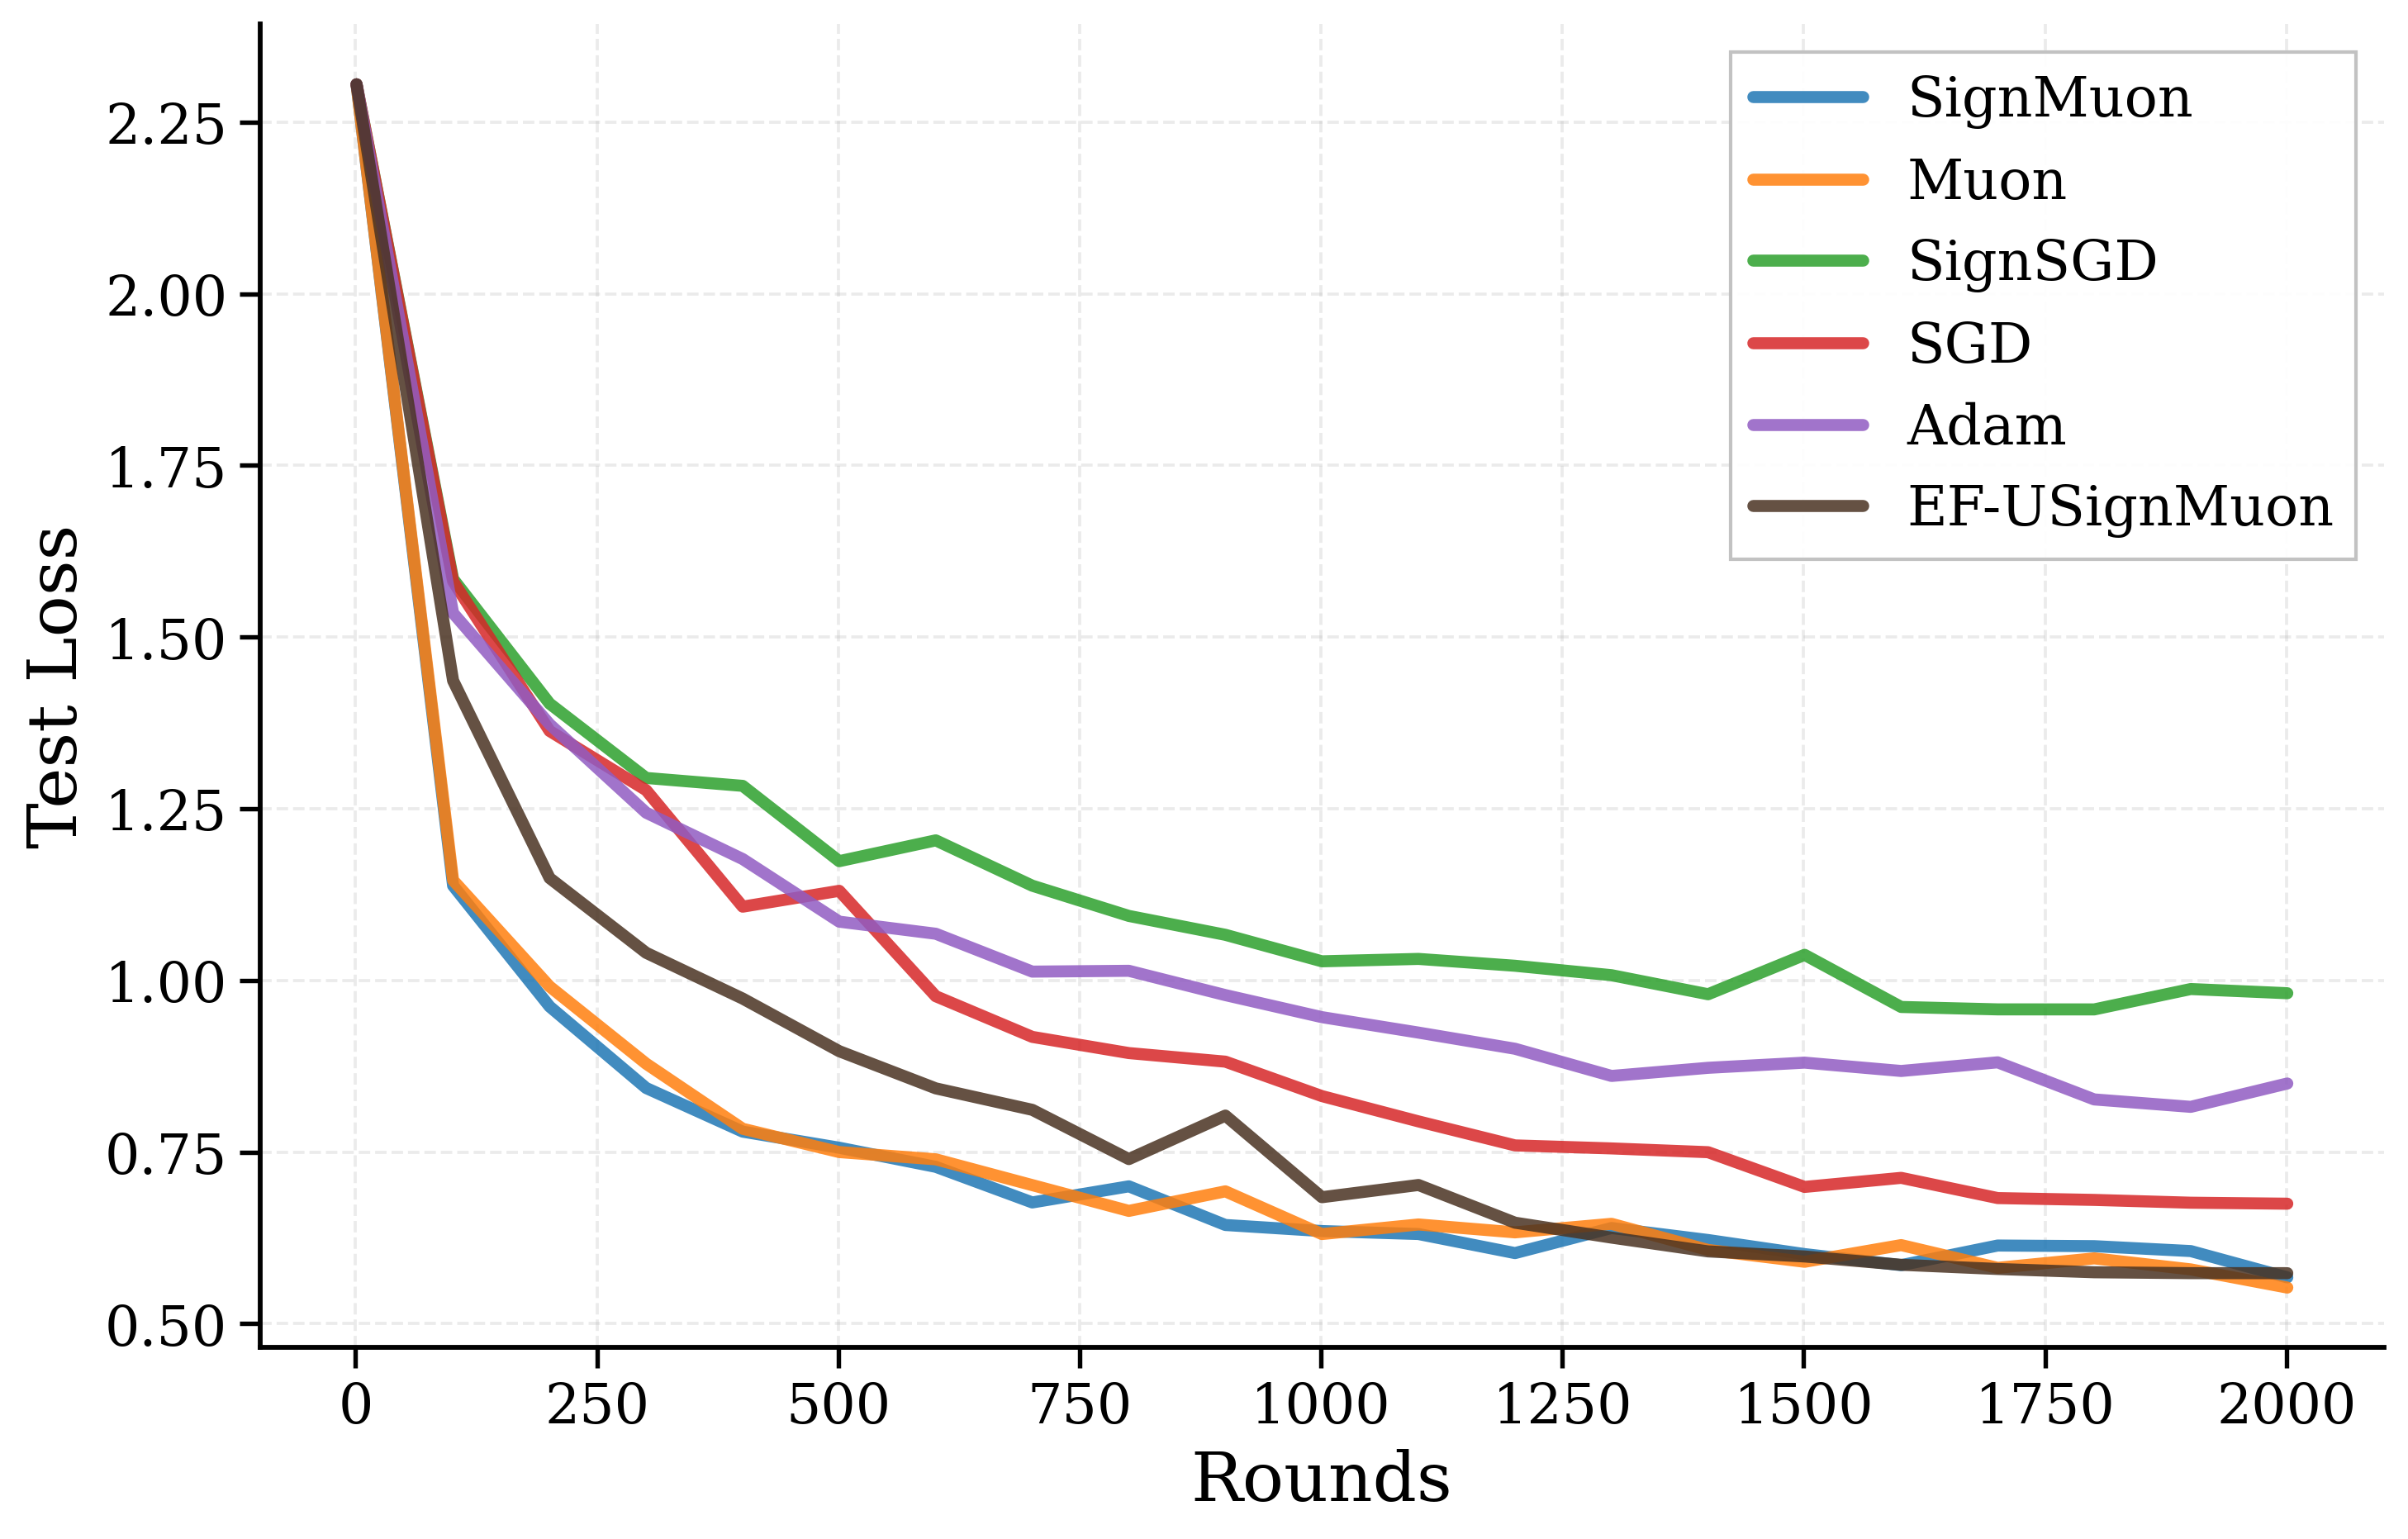
\includegraphics[width=\textwidth]{images/federated_images/3_1_loss.png} 
        \caption{Test Loss}
    \end{subfigure}
    \hfill
    \begin{subfigure}[b]{0.48\textwidth}
        \centering
        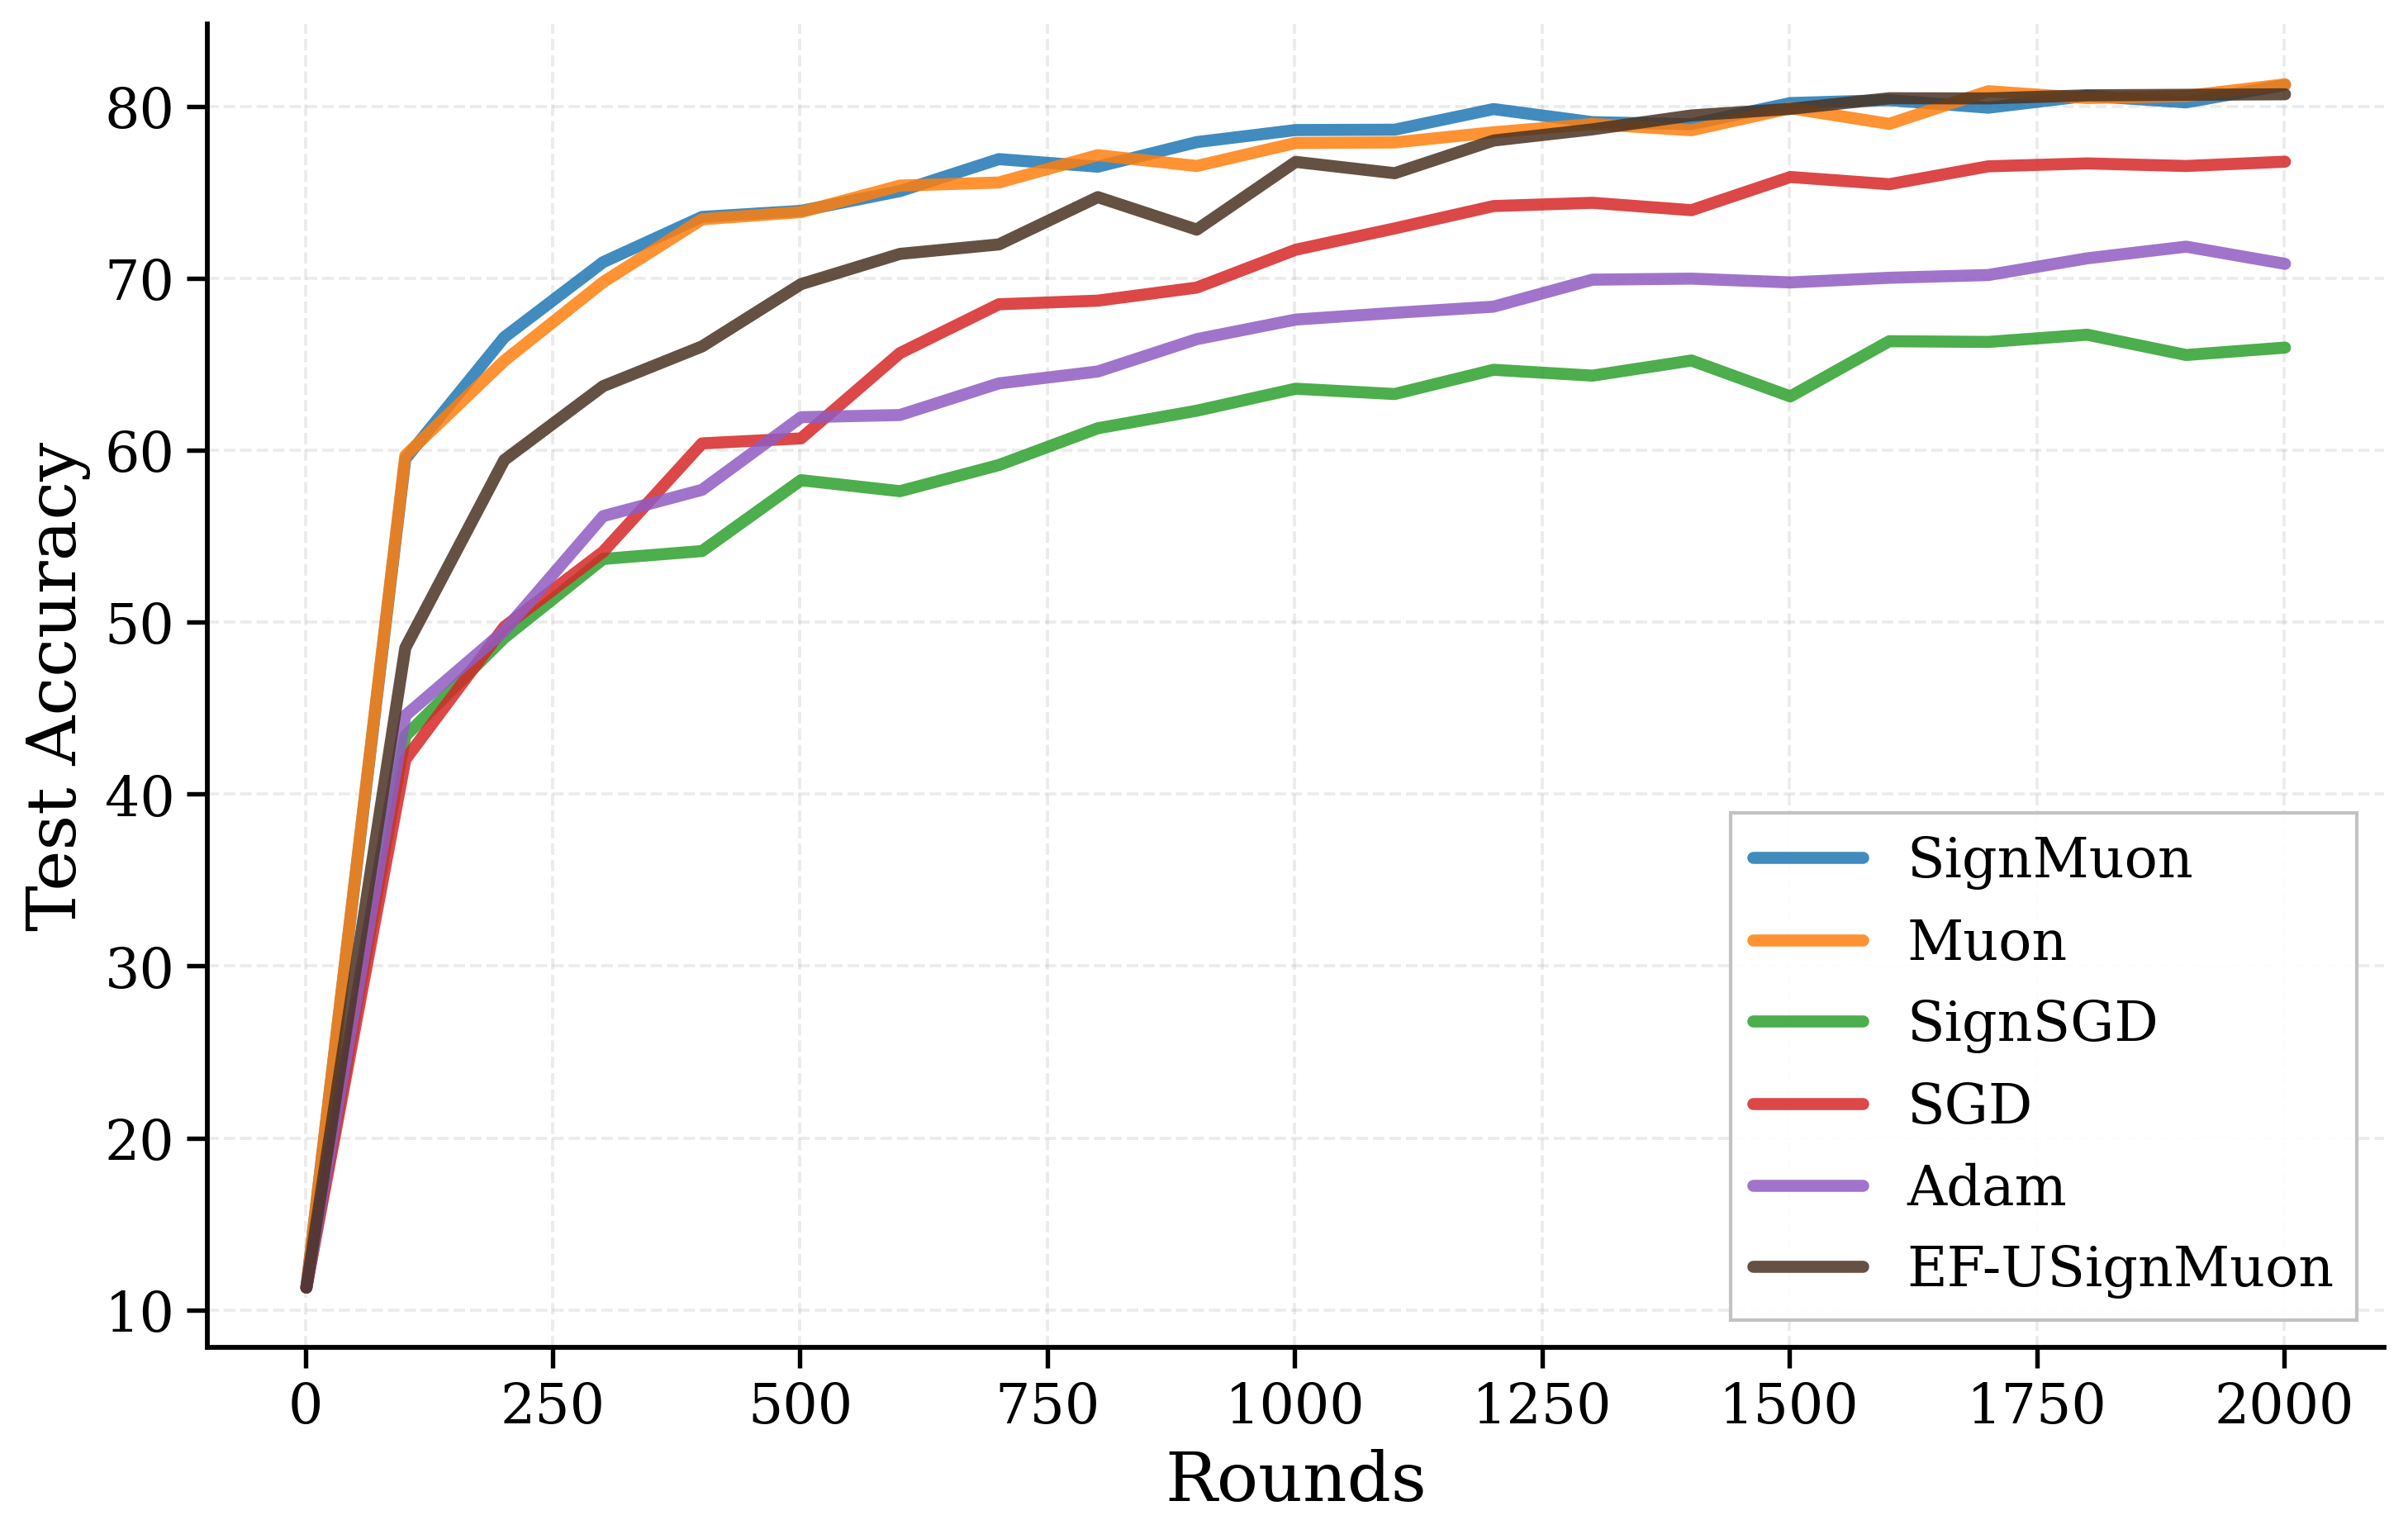
\includegraphics[width=\textwidth]{images/federated_images/3_1_acc.png}
        \caption{Test Accuracy}
    \end{subfigure}
    \caption{CIFAR-10 Federated Learning on CNN2. Experiment 2: Comparison of Optimization Algorithms with (N = 3) Clients.}
    \label{fig:exp_2}
\end{figure*}

\subsection{Federated training results. Experiment 3}\label{app:results_fed:3}
Figure~\ref{fig:exp_3} (together with Table~\ref{tab:exp_3} in the main text) reports the comparison of optimizers with $N=10$ clients (Experiment~3).
\begin{figure*}[!t]
    \centering
    \begin{subfigure}[b]{0.48\textwidth}
        \centering
        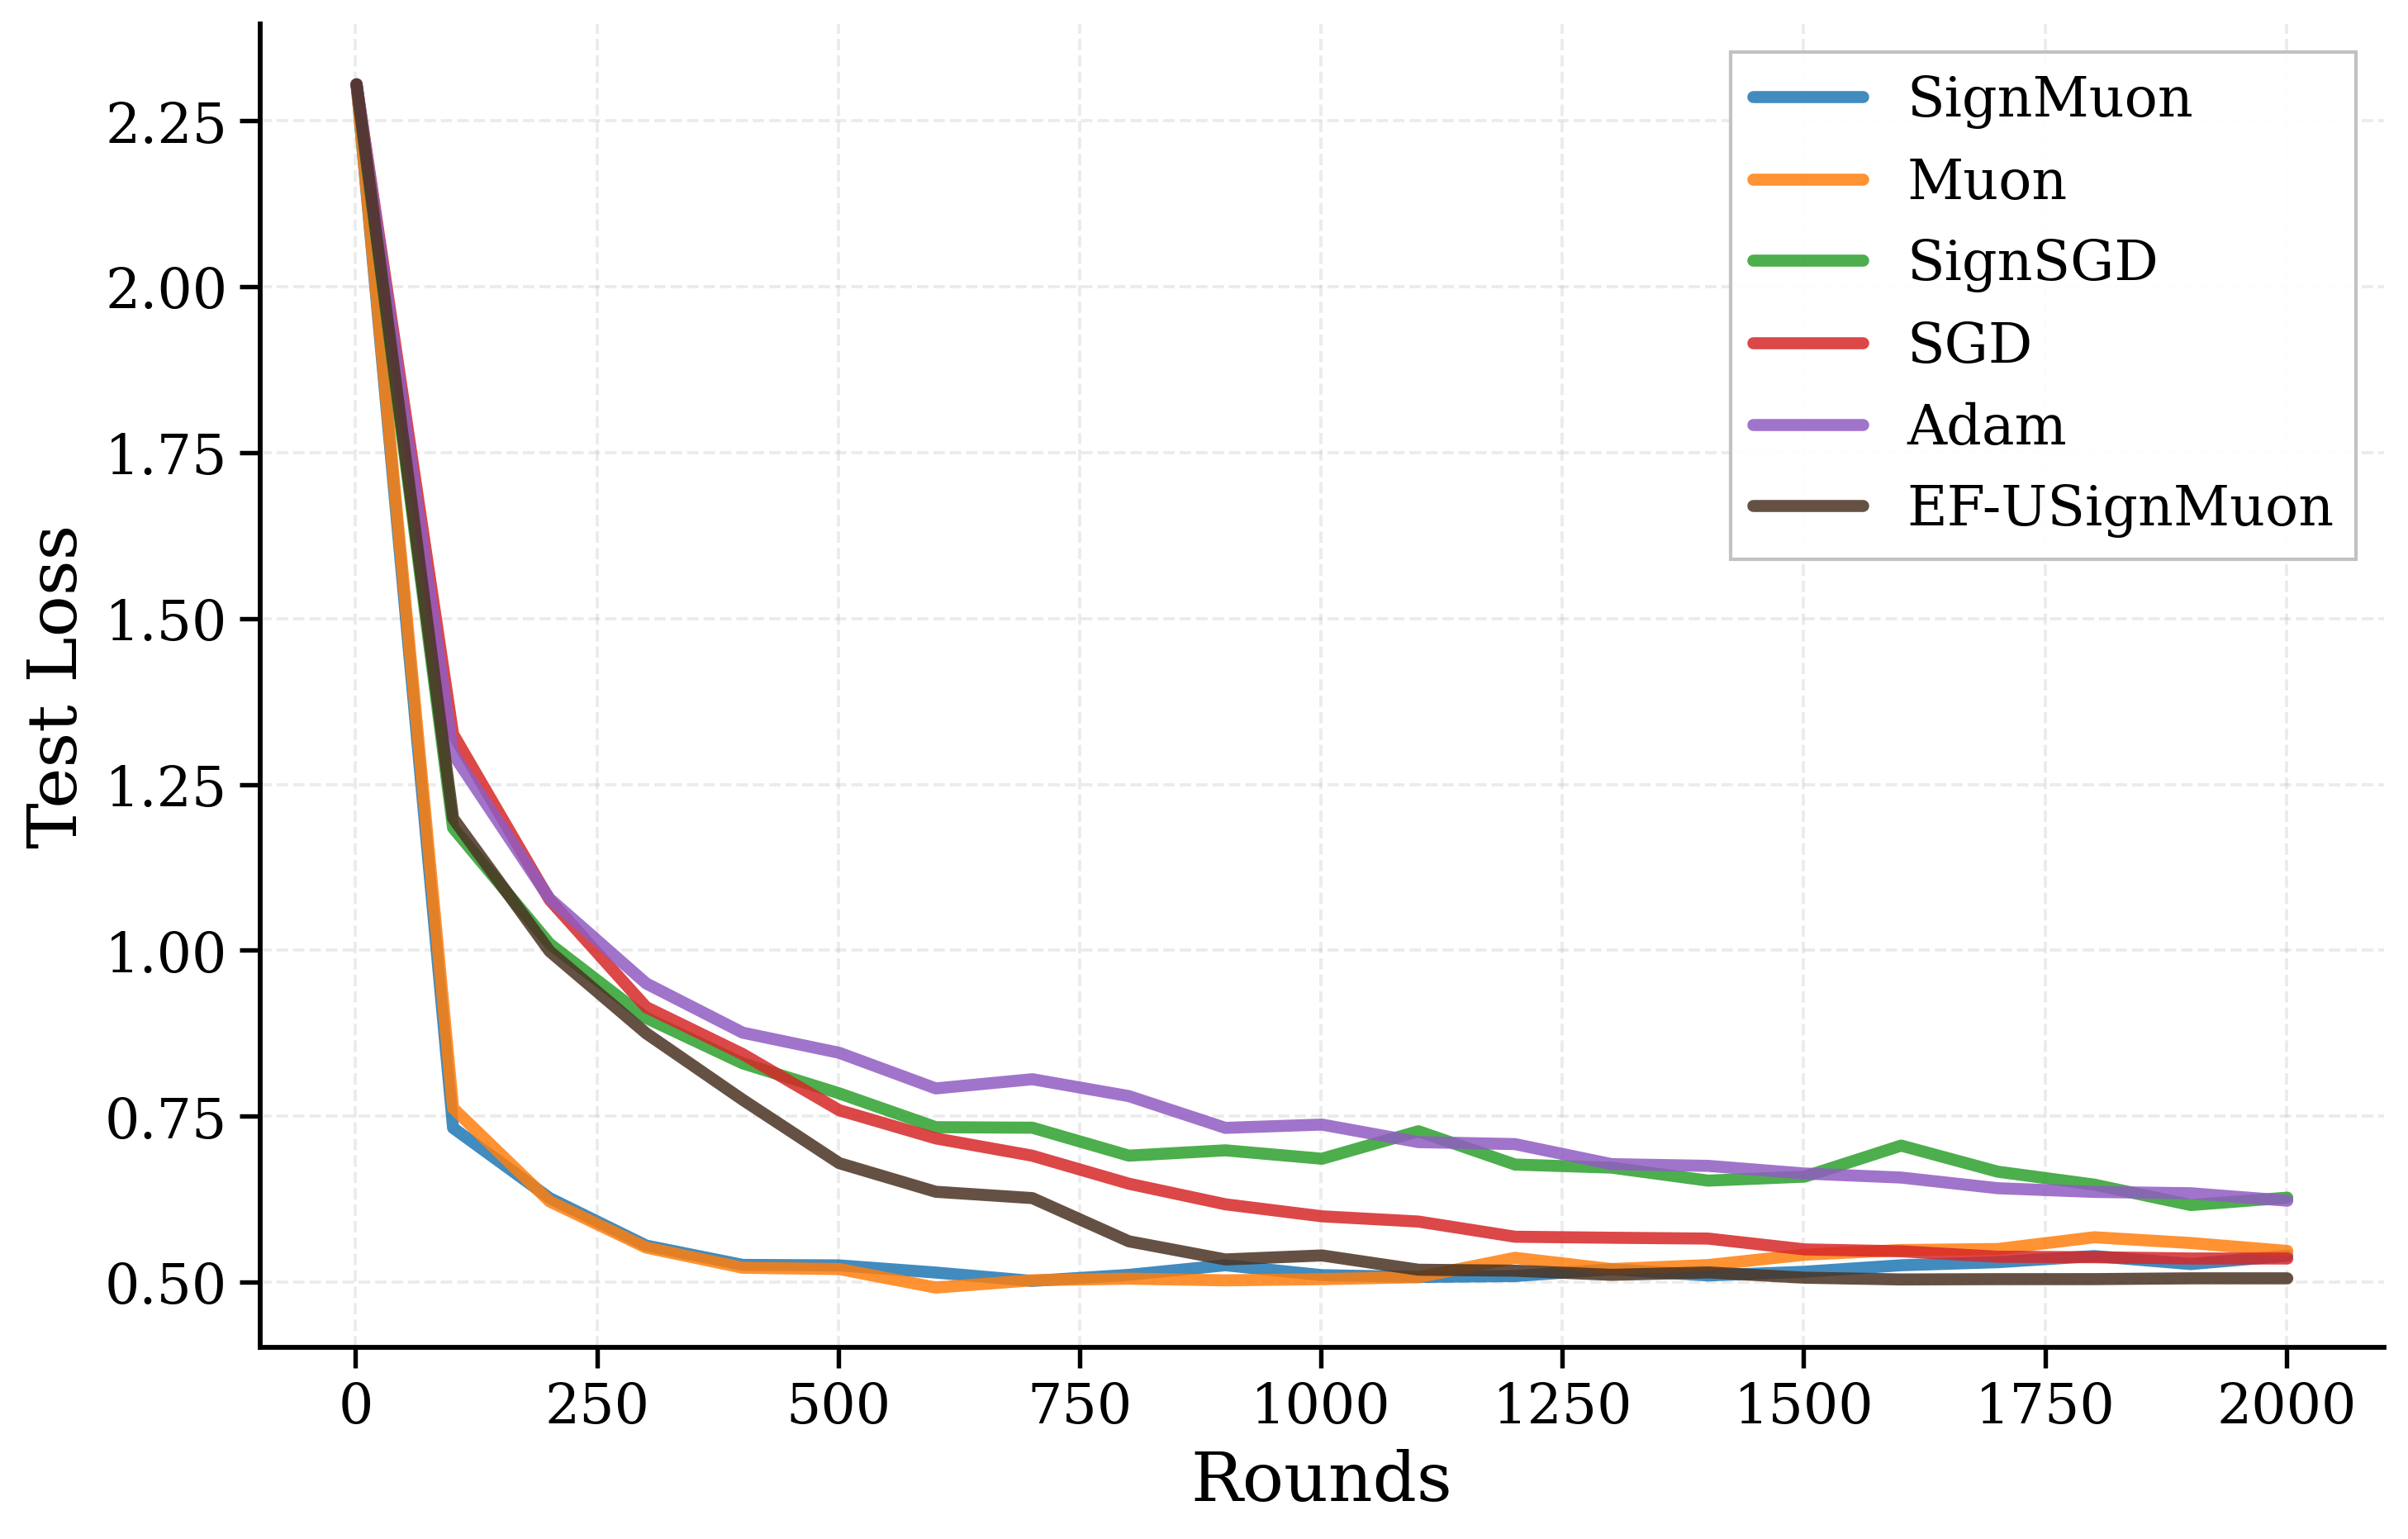
\includegraphics[width=\textwidth]{images/federated_images/10_3_loss.png} 
        \caption{Test Loss}
    \end{subfigure}
    \hfill
    \begin{subfigure}[b]{0.48\textwidth}
        \centering
        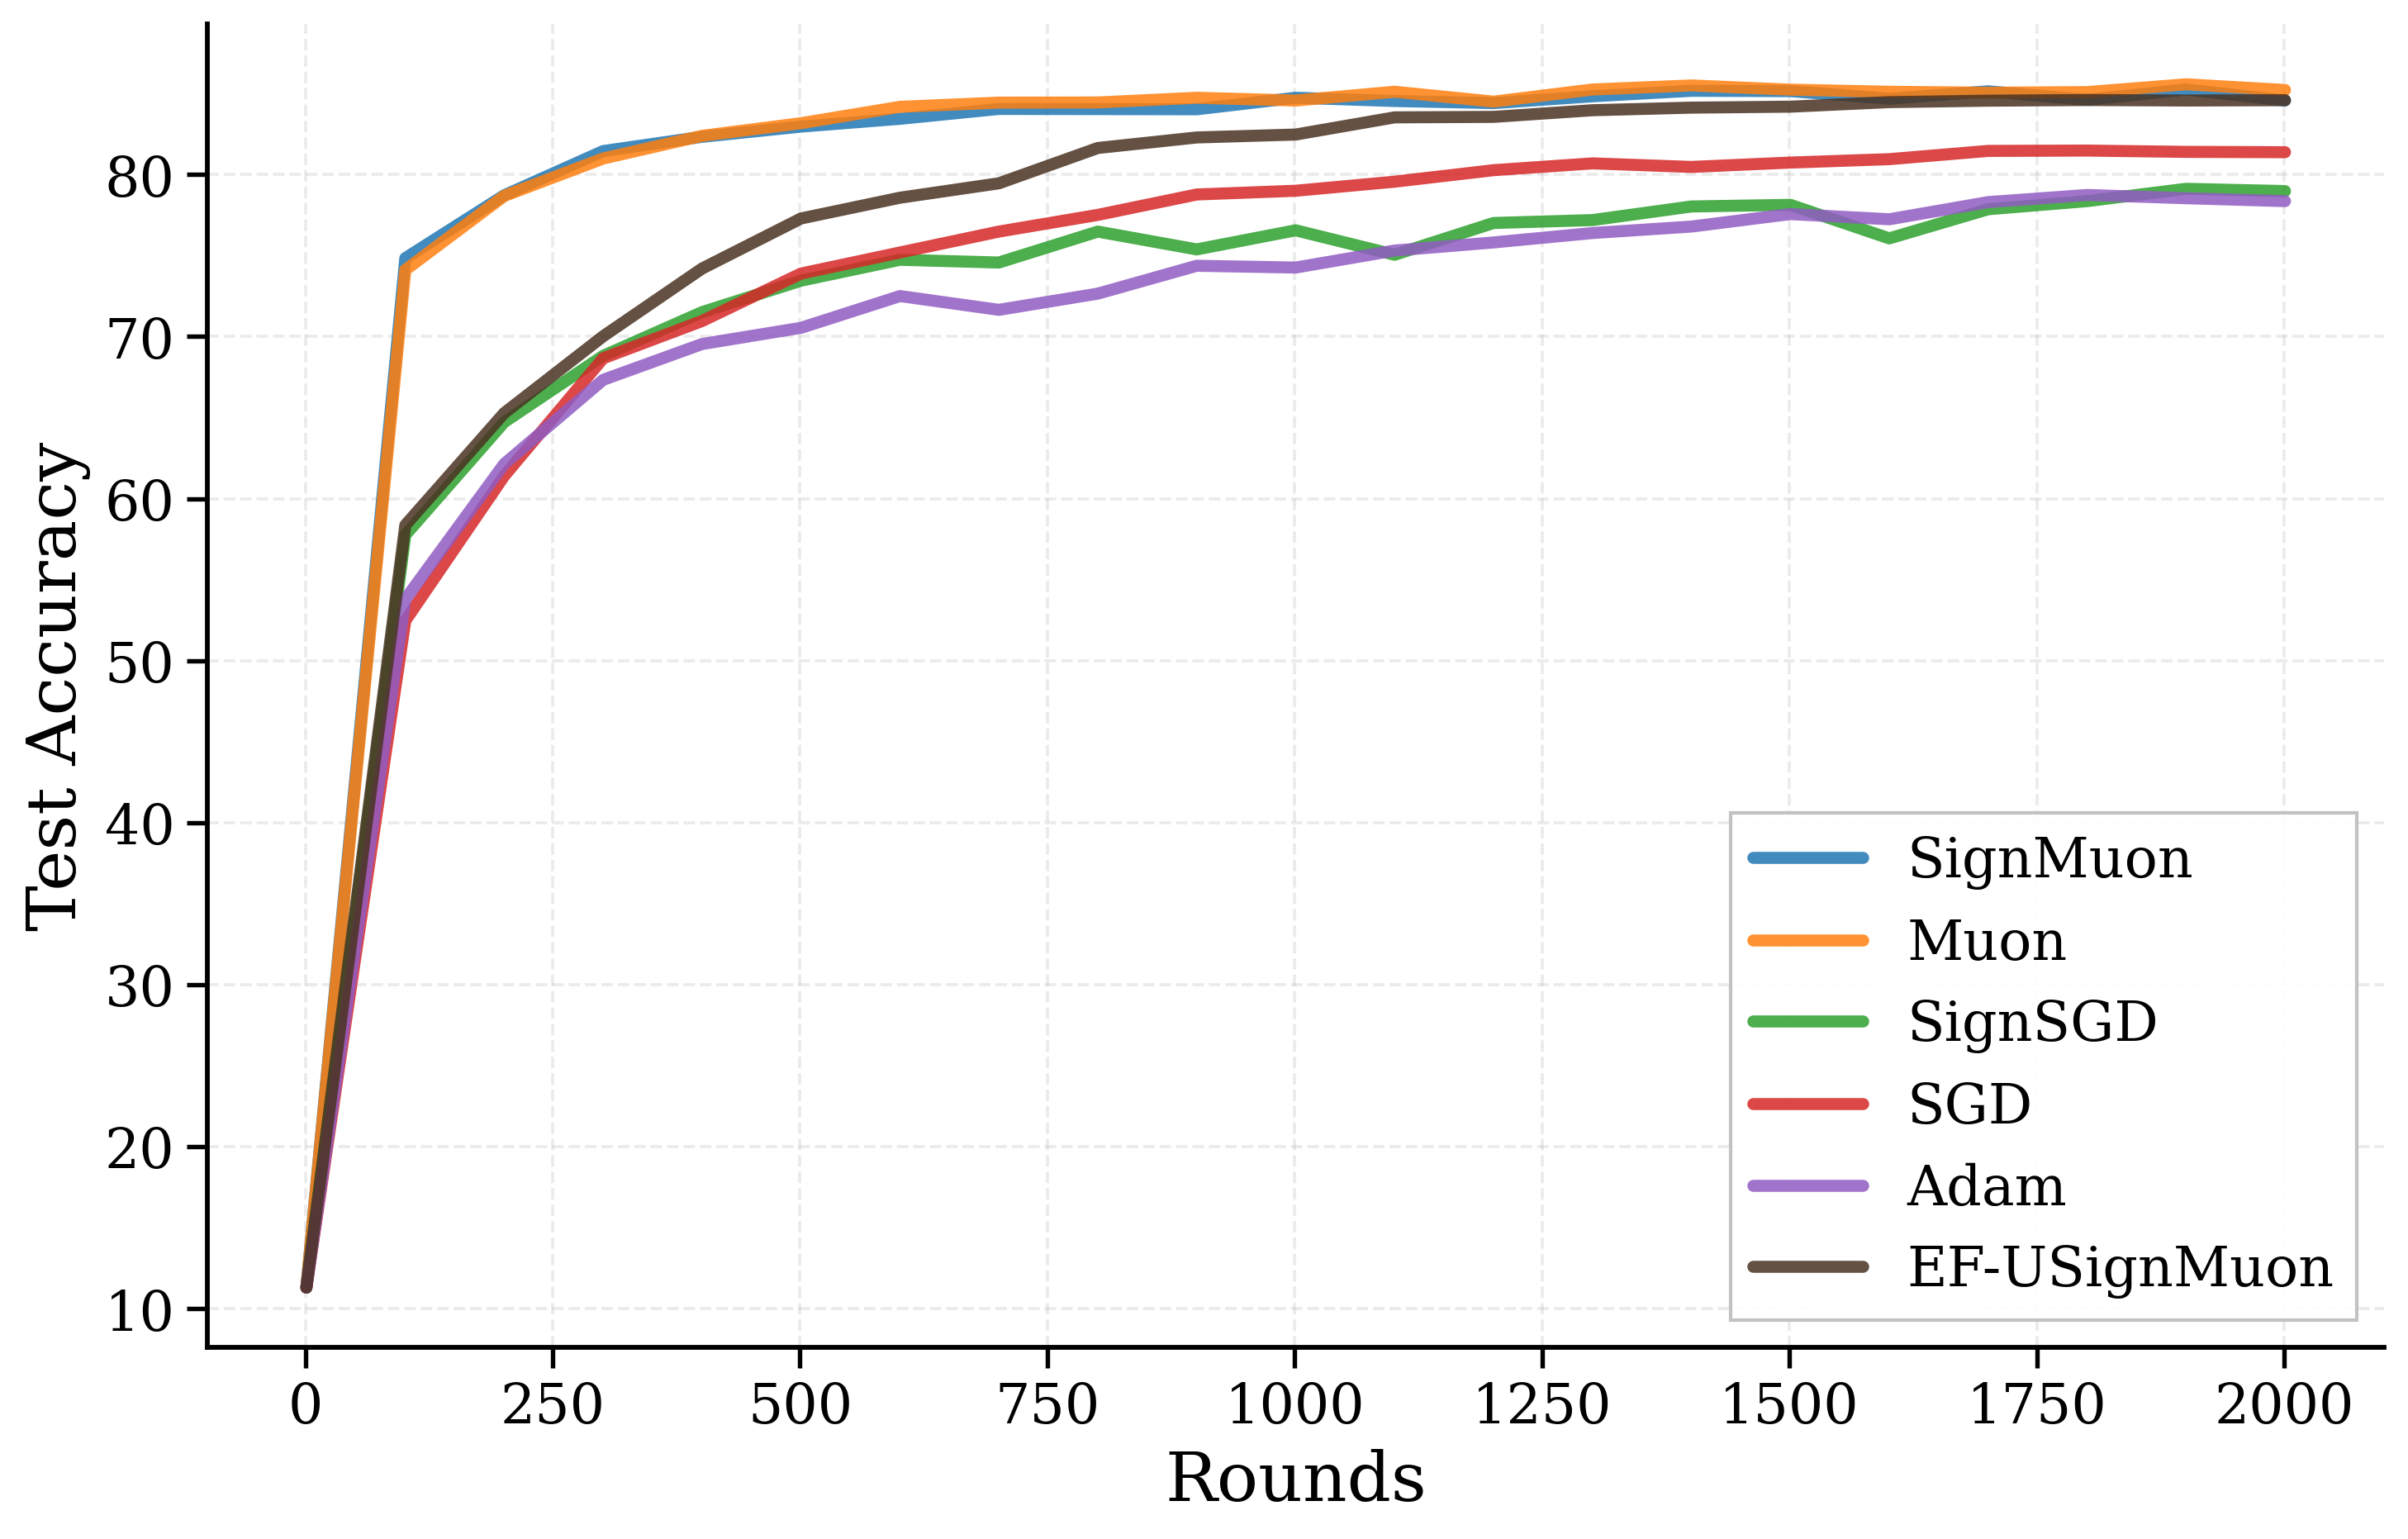
\includegraphics[width=\textwidth]{images/federated_images/10_3_acc.png}
        \caption{Test Accuracy}
    \end{subfigure}
    \caption{CIFAR-10 Federated Learning on CNN2. Experiment 3: Comparison of Optimization Algorithms with (N = 10) Clients.}
    \label{fig:exp_3}
\end{figure*}


\subsection{Algorithms}\label{app:alg}

\begin{algorithm}[!t]
\caption{MuonLMO}
\label{alg:muon_lmo}
\begin{algorithmic}[1]
\Statex \textbf{Input}: tensor $\mathbf{Y}$; Newton-Schulz coefficients $a=3.4445,\,b=4.7750,\,c=2.0315$; iteration count $\mathrm{ns\_steps}$
\Statex \textbf{Output}: Muon LMO direction $\mathbf{D}\approx\mathbf{U}\mathbf{V}^\top$ of $\mathbf{Y}$
\State $\mathbf{Y} \gets \text{ReshapeTo2D}(\mathbf{Y})$ \Comment{Flatten tensor to matrix $m \times n$}
\State $\mathbf{Y} \gets \mathbf{Y}/\|\mathbf{Y}\|_F$ \Comment{Normalize (optional)}
\For{$k = 1$ to $\mathrm{ns\_steps}$} \Comment{5th-order Newton-Schulz orthogonalization}
    \State $\mathbf{A} \gets \mathbf{Y}\mathbf{Y}^\top$
    \State $\mathbf{Y} \gets a\,\mathbf{Y} - b\,\mathbf{A}\mathbf{Y} + c\,\mathbf{A}^2\,\mathbf{Y}$
\EndFor
\State $\mathbf{D} \gets \text{ReshapeToOriginal}(\mathbf{Y})$ \Comment{Reshape back to the original tensor shape}
\State \Return $\mathbf{D}$
\end{algorithmic}
\end{algorithm}

\begin{algorithm}
\caption{Centralized SignMuon}
\label{central_alg}
\textbf{Input}: Initial model $\mathbf{X}_0$, initial gradient $\mathbf{G}_0$, momentum coefficient $\mu$, learning rate $\eta_t$ \\
\textbf{Output}: Updated model $\mathbf{X}$ 
\begin{algorithmic}[1]
\State $\mathbf{M}_0 \gets 0$ 
\For{$t = 0$ to $(T - 1)$}
    \State Stochastic gradient $\mathbf{G}_t$
    \State $\mathbf{M}_t \gets \mu \mathbf{M}_{t-1} + \mathbf{G}_t$ \Comment{Momentum accumulation}
    \State $\tilde{\mathbf{M}}_t =
    \begin{cases} 
        \mathbf{G}_t + \mu \mathbf{M}_t, & \text{(Nesterov momentum)}, \\
        \mathbf{M}_t, & \text{(otherwise)}
    \end{cases}$
    \State $\mathbf{D}_t \gets \mathrm{MuonLMO}(\tilde{\mathbf{M}}_t)$ \Comment{Algorithm~\ref{alg:muon_lmo}}
    \State $\mathbf{s}_t \gets \operatorname{sign}(\mathbf{D}_t)$ \Comment{Sign compression}
    \State $\mathbf{X}_{t+1} \gets \mathbf{X}_t - \eta_t \mathbf{s}_t$ \Comment{Update parameters}
\EndFor
\end{algorithmic}
\end{algorithm}


\begin{algorithm}[!ht]
    \caption{Centralized EF21-SignMuon}
    \label{alg:central_ef21_signmuon}
    \textbf{Input}: Initial model $\mathbf{X}_0$, initial gradient $\mathbf{G}_0$, momentum coefficient $\mu$, learning rate $\eta_t$ \\
    \textbf{Output}: Updated model $\mathbf{X}$
    \begin{algorithmic}[1]
    \State $\mathbf{M}_0 \gets 0,\quad \mathbf{d}_0^{\mathrm{est}} \gets 0$
    \For{$t = 0$ to $(T - 1)$}
      \State Stochastic gradient $\mathbf{G}_t$
      \State $\mathbf{M}_t \gets \mu\mathbf{M}_{t-1} + \mathbf{G}_t$ \Comment{Momentum accumulation}
      \State $\mathbf{D}_t \gets \mathrm{MuonLMO}(\mathbf{M}_t)$ \Comment{Apply exact LMO first (Algorithm~\ref{alg:muon_lmo})}
      \State $\Delta_t \gets \mathbf{D}_t - \mathbf{d}_t^{\mathrm{est}}$ \Comment{Compute residual of LMO direction}
      \State $\alpha_t \gets \operatorname{mean}(|\Delta_t|)$ \Comment{Adaptive scaling factor}
      \State $\mathbf{d}_{t+1}^{\mathrm{est}} \gets \mathbf{d}_t^{\mathrm{est}} + \alpha_t\operatorname{sign}(\Delta_t)$ \Comment{Uplink EF21 estimator (1-bit residual)}
      \State $\mathbf{X}_{t+1} \gets \mathbf{X}_t - \eta_t\mathbf{d}_{t+1}^{\mathrm{est}}$ \Comment{Update parameters}
    \EndFor
    \end{algorithmic}
\end{algorithm}

\begin{algorithm}[!h]
    \caption{Centralized MuonUSign}
    \label{alg:muon_usign}
    \textbf{Input}: Initial model $\mathbf{X}_0$, initial gradient $\mathbf{G}_0$, momentum coefficient $\mu$, learning rate $\eta_t$ \\
    \textbf{Output}: Updated model $\mathbf{X}$ 
    \begin{algorithmic}[1]
    \State $\mathbf{M}_0 \gets 0$ 
    \For{$t = 0$ to $(T - 1)$}
        \State Stochastic gradient $\mathbf{G}_t$
        \State $\mathbf{M}_t \gets \mu \mathbf{M}_{t-1} + \mathbf{G}_t$ \Comment{Momentum accumulation}
        \State $\tilde{\mathbf{M}}_t =
        \begin{cases} 
            \mathbf{G}_t + \mu \mathbf{M}_t, & \text{(Nesterov momentum)}, \\
            \mathbf{M}_t, & \text{(otherwise)}
        \end{cases}$
        \State $\mathbf{s}_t \gets \operatorname{sign}(\tilde{\mathbf{M}}_t)$ \Comment{Uplink sign compression}
        \State $\mathbf{D}_t \gets \mathrm{MuonLMO}(\mathbf{s}_t)$ \Comment{Algorithm~\ref{alg:muon_lmo}}
        \State $\mathbf{X}_{t+1} \gets \mathbf{X}_t - \eta_t \mathbf{D}_t$ \Comment{Update parameters}
    \EndFor
    \end{algorithmic}
    \end{algorithm}

    \begin{algorithm}[!h]
        \caption{Centralized MuonUDSign (bidirectional)}
        \label{alg:muon_udsign}
        \textbf{Input}: Initial model $\mathbf{X}_0$, initial gradient $\mathbf{G}_0$, momentum coefficient $\mu$, learning rate $\eta_t$ \\
        \textbf{Output}: Updated model $\mathbf{X}$ 
        \begin{algorithmic}[1]
        \State $\mathbf{M}_0 \gets 0$ 
        \For{$t = 0$ to $(T - 1)$}
            \State Stochastic gradient $\mathbf{G}_t$
            \State $\mathbf{M}_t \gets \mu \mathbf{M}_{t-1} + \mathbf{G}_t$ \Comment{Momentum accumulation}
            \State $\tilde{\mathbf{M}}_t =
            \begin{cases} 
                \mathbf{G}_t + \mu \mathbf{M}_t, & \text{(Nesterov momentum)}, \\
                \mathbf{M}_t, & \text{(otherwise)}
            \end{cases}$
            \State $\mathbf{S}_t^{\uparrow} \gets \operatorname{sign}(\tilde{\mathbf{M}}_t)$ \Comment{Uplink sign compression}
            \State $\mathbf{D}_t \gets \mathrm{MuonLMO}(\mathbf{S}_t^{\uparrow})$ \Comment{Server LMO (Algorithm~\ref{alg:muon_lmo})}
            \State $\mathbf{S}_t^{\downarrow} \gets \operatorname{sign}(\mathbf{D}_t)$ \Comment{Downlink sign compression}
            \State $\mathbf{X}_{t+1} \gets \mathbf{X}_t - \eta_t \mathbf{S}_t^{\downarrow}$ \Comment{Update parameters}
        \EndFor
        \end{algorithmic}
\end{algorithm}
    
\begin{algorithm}[!t]
\caption{Centralized EF21-MuonUSign}
\label{central_alg_ef}
\textbf{Input}: Initial model $\mathbf{X}_0$, initial gradient $\mathbf{G}_0$, momentum coefficient $\mu$, learning rate $\eta_t$ \\
\textbf{Output}: Updated model $\mathbf{X}$
\begin{algorithmic}[1]
\State $\mathbf{M}_0 \gets 0,\quad \mathbf{g}_0^{\mathrm{est}} \gets 0$
\For{$t = 0$ to $(T - 1)$}
  \State Stochastic gradient $\mathbf{G}_t$
  \State $\mathbf{M}_t \gets \mu\mathbf{M}_{t-1} + \mathbf{G}_t$
  \State $\Delta_t \gets \mathbf{M}_t - \mathbf{g}_t^{\mathrm{est}}$;
  \quad $\alpha_t \gets \operatorname{mean}(|\Delta_t|)$;
  \State $\mathbf{g}_{t+1}^{\mathrm{est}} \gets \mathbf{g}_t^{\mathrm{est}} + \alpha_t\operatorname{sign}(\Delta_t)$
         \Comment{Uplink EF21 estimator (1-bit residual)}
  \State $\mathbf{D}_t \gets \mathrm{MuonLMO}(\mathbf{g}_{t+1}^{\mathrm{est}})$
         \Comment{Algorithm~\ref{alg:muon_lmo}}
  \State $\mathbf{X}_{t+1} \gets \mathbf{X}_t - \eta_t\mathbf{D}_t$
\EndFor
\end{algorithmic}
\end{algorithm}

\begin{algorithm}[!t]
\caption{Centralized EF21-MuonUDSign (bidirectional)}
\label{central_alg_ud}
\textbf{Input}: Initial model $\mathbf{X}_0=\mathbf{W}_0$,  initial gradient $\mathbf{G}_0$, momentum coefficient $\mu$, learning rate $\eta_t$ \\
\textbf{Output}: Updated model $\mathbf{X}$
\begin{algorithmic}[1]
\State $\mathbf{M}_0 \gets 0,\quad \mathbf{g}_0^{\mathrm{est}} \gets 0$
\For{$t = 0$ to $(T - 1)$}
\State Stochastic gradient $\mathbf{G}_t$ at the broadcast model $\mathbf{W}_t$
\State $\mathbf{M}_t \gets \mu\mathbf{M}_{t-1} + \mathbf{G}_t$ \Comment{Momentum}
\State $\Delta_t^{\uparrow} \gets \mathbf{M}_t - \mathbf{g}_t^{\mathrm{est}}$
\State $\alpha_t^{\uparrow} \gets
\operatorname{mean}(|\Delta_t^{\uparrow}|)$
\State $\mathbf{g}_{t+1}^{\mathrm{est}} \gets \mathbf{g}_t^{\mathrm{est}} +
\alpha_t^{\uparrow}\operatorname{sign}(\Delta_t^{\uparrow})$
       \Comment{Uplink EF21 estimator (1-bit)}
\State $\mathbf{D}_t \gets \mathrm{MuonLMO}(\mathbf{g}_{t+1}^{\mathrm{est}})$ \Comment{Algorithm~\ref{alg:muon_lmo}}
\State $\mathbf{X}_{t+1} \gets \mathbf{X}_t - \eta_t\mathbf{D}_t$
\State $\Delta_t^{\downarrow} \gets \mathbf{X}_{t+1} - \mathbf{W}_t$
\State $\alpha_t^{\downarrow} \gets
\operatorname{mean}(|\Delta_t^{\downarrow}|)$
\State $\mathbf{W}_{t+1} \gets \mathbf{W}_t + \alpha_t^{\downarrow}\operatorname{sign}(\Delta_t^{\downarrow})$
       \Comment{Downlink EF (1-bit model increment)}
\EndFor
\end{algorithmic}
\end{algorithm}


\begin{algorithm}[!t]
\caption{Federated SignMuon}
\label{fed_alg}
\textbf{Input}: Initial model $\mathbf{X}_0$, clients number $N$, rounds number $\mathrm{rounds}$, local steps number $\mathrm{n\_steps}$, learning rate for the main layers $\eta_t$, learning rate for the last layer $\eta_t^{\text{aux}}$, momentum coefficient $\mu$ \\
\textbf{Output}: Updated global model $\mathbf{X}$
\begin{algorithmic}[1]
\For{$j = 1$ to $N$} \State $\mathbf{M}_0^{(j)} \gets 0$ \Comment{Initialization of local buffers on clients}
\EndFor
\State Initialize AdamW for last\_layer with learning rate $\eta^{\mathrm{aux}}_0$
\For{$t = 0$ to $(\mathrm{rounds} - 1)$}
    \For{$j = 1$ to $N$ \textbf{in parallel}} 
        \State $\mathbf{X}_t^{(j)} \gets \mathbf{X}_t$ \Comment{Retrieve global model}
        \For{$k = 1$ to $\mathrm{n\_steps}$}
            \State Sample a batch $\xi_{t,k}^{(j)}$
            \State $\nabla f_k \gets \nabla f(\mathbf{X}_t^{(j)}; \xi_{t,k}^{(j)})$
            \State $\mathbf{G}_t^{(j)} \gets \mathbf{G}_t^{(j)} + \nabla f_k$
        \EndFor
        \\ \State $\mathbf{G}_t^{(j)} \gets \mathbf{G}_t^{(j)} / \mathrm{n\_steps}$ \Comment{Gradient averaging}
        \State $\mathbf{M}_t^{(j)} \gets \mu \mathbf{M}_{t-1}^{(j)} + \mathbf{G}_t^{(j)}$ \Comment{Local momentum update}
        \State $\mathbf{D}_t^{(j)} \gets \mathrm{MuonLMO}(\mathbf{M}_t^{(j)})$ \Comment{Algorithm~\ref{alg:muon_lmo}}
        \State $\mathbf{s}_t^{(j)} \gets \operatorname{sign}\bigl(\mathbf{D}_t^{(j)}\bigr)$ \Comment{Sign compression}
        \\\State \textbf{Send $\mathbf{s}_t^{(j)}$ to server} \For{\textbf{each} $\mathbf{W}^{\text{last}}$ \textbf{in last\_layer}}
          \State Send $\mathbf{G}_t^{(j)}$ to the server \Comment{Raw gradient for the head}
        \EndFor
      \EndFor
      \State $\mathbf{s}_t^{\mathrm{agg}} \gets \operatorname{sign}\!\left(\sum_{j=1}^{N} \mathbf{s}_t^{(j)}\right)$ \Comment{Majority vote
      (matrix layers)}
      \State $\bar{\mathbf{G}}_t^{\text{last}} \gets \frac{1}{N}\sum_{j=1}^{N} \mathbf{G}_t^{(j)}$ \Comment{Average raw gradient for the   
      head}
      \State $\mathbf{X}_{t+1} \gets \mathbf{X}_t - \eta_t \mathbf{s}_t^{\mathrm{agg}}$ \Comment{Matrix parameter update}
      \\ \State $\mathbf{X}_{t+1}^{\text{last}} \gets \text{AdamW}(\mathbf{X}_t^{\text{last}}, \bar{\mathbf{G}}_t^{\text{last}}, \eta_t^{\text{aux}})$ \Comment{AdamW on the averaged gradient}
\EndFor
\State \Return $\mathbf{X}_{\mathrm{rounds}}$
\end{algorithmic}
\end{algorithm}


\begin{algorithm}[!t]
\caption{Federated EF21-MuonUSign}
\label{ef21_alg}
\textbf{Input}: Initial model $\mathbf{X}_0$, clients number $N$, rounds number $\mathrm{rounds}$, local steps number $\mathrm{n\_steps}$, learning rate for the main layers $\eta_t$, learning rate for the last layer $\eta_t^{\text{aux}}$,  momentum coefficient $\mu$ \\
\textbf{Output}: Updated global model $\mathbf{X}$
\begin{algorithmic}[1]
\State $\mathbf{G}_0 \gets 0$ \Comment{Initialize the global gradient estimate on the server (for the main layers)}
\For{$j = 1$ to $N$} 
    \State $\mathbf{g}_0^{(j)} \gets 0, \; \mathbf{M}_0^{(j)} \gets 0$ \Comment{Initialize local estimators and momentum}
\EndFor
\State Initialize AdamW for last\_layer with learning rate $\eta^{\mathrm{aux}}_0$
\For{$t = 0$ to $(\mathrm{rounds} - 1)$}

    \For{$j = 1$ to $N$ \textbf{in parallel}} \Comment{Local step of EF21}
        \State $\mathbf{X}_t^{(j)} \gets \mathbf{X}_t$ \Comment{Retrieve global model}
        \State $\mathbf{G}_t^{(j)} \gets 0$
        \For{$k = 1$ to $\mathrm{n\_steps}$}
            \State Sample a batch $\xi_{t,k}^{(j)}$
            \State $\nabla f_k \gets \nabla f(\mathbf{X}_t^{(j)}; \xi_{t,k}^{(j)})$
            \State $\mathbf{G}_t^{(j)} \gets \mathbf{G}_t^{(j)} + \nabla f_k$
        \EndFor
        \State $\mathbf{G}_t^{(j)} \gets \mathbf{G}_t^{(j)} / \mathrm{n\_steps}$ \Comment{Gradient averaging}
        
        \State $\mathbf{M}_t^{(j)} \gets \mu \mathbf{M}_{t-1}^{(j)} + \mathbf{G}_t^{(j)}$ \Comment{Local momentum update}
        
        \For{\textbf{each} parameter $\mathbf{W}$ \textbf{not in last\_layer}}
            \State $\Delta_t^{(j)} \gets \mathbf{M}_t^{(j)} - \mathbf{g}_t^{(j)}$ \Comment{Difference computation}
            \State $\alpha_t^{(j)} \gets \operatorname{mean}(|\Delta_t^{(j)}|)$ \Comment{Adaptive scaling factor}
            \State $\mathbf{s}_t^{(j)} \gets \operatorname{sign}(\Delta_t^{(j)})$ \Comment{Compress shifted gradient}
            \State $\mathbf{g}_{t+1}^{(j)} \gets \mathbf{g}_t^{(j)} + \alpha_t^{(j)} \mathbf{s}_t^{(j)}$ \Comment{Compute gradient estimator}
            \State Send $(\mathbf{s}_t^{(j)}, \alpha_t^{(j)})$ to the server
        \EndFor
        
        \For{\textbf{each} parameters $\mathbf{W}^{\text{last}}$ \textbf{in last\_layer}}
            \State Send $\mathbf{G}_t^{(j)}$ to the server
        \EndFor
    \EndFor
    \State $\mathbf{G}_{t+1} \gets \mathbf{G}_t + \frac{1}{N} \sum_{j=1}^N \alpha_t^{(j)} \mathbf{s}_t^{(j)}$ \Comment{Update the global estimator on the server}
    \For{\textbf{each} parameters $\mathbf{X}$}
        \State $\mathbf{D}_{t+1} \gets \mathrm{MuonLMO}(\mathbf{G}_{t+1})$ \Comment{Algorithm~\ref{alg:muon_lmo}}
        \State $\mathbf{X}_{t+1} \gets \mathbf{X}_t - \eta_t \mathbf{D}_{t+1}$ \Comment{Update the matrix parameters}
    \EndFor
    \State $\nabla^{\text{last}} \gets \frac{1}{N} \sum_{j=1}^N \mathbf{G}_t^{(j)}$
    \State $\mathbf{X}_{t+1}^{\text{last}} \gets \text{AdamW}(\mathbf{X}_t^{\text{last}}, \nabla^{\text{last}}, \eta_t^{\text{aux}})$ \Comment{Classifier update}
\EndFor
\State \Return $\mathbf{X}_{\mathrm{rounds}}$
\end{algorithmic}
\end{algorithm}


%%%%%%%%%%%%%%%%%%%%%%%%%%%%%%%%%%%%%%%%%%%%%%%%%%%%%%%%%%%%
% References (placed after the Appendix; see note above).
% \bibliographystyle{unsrtnat}  % aaai2027.sty sets the style to aaai2027.bst automatically
\bibliography{references}

\end{document}